%%%%%%%%%%%%%%%%%%%%%%%%%%%%%%%%%%%%%%%%%%%%%%%%%%%%%%%%%%%%%%%%%%%%%%%%%%%%
% AGUJournalTemplate.tex: this template file is for articles formatted with LaTeX
%
% This file includes commands and instructions
% given in the order necessary to produce a final output that will
% satisfy AGU requirements, including customized APA reference formatting.
%
% You may copy this file and give it your
% article name, and enter your text.
%
% guidelines and troubleshooting are here: 

%% To submit your paper:
\documentclass[draft]{agujournal2019}
\usepackage{url} %this package should fix any errors with URLs in refs.
\usepackage{lineno}
\usepackage[inline]{trackchanges} %for better track changes. finalnew option will compile document with changes incorporated.
\usepackage{soul}
\usepackage{framed}
\usepackage{amsmath}
\usepackage{amsfonts}
\usepackage{comment}
\newcommand{\bs}{\boldsymbol{s}}
\newcommand{\bg}{\boldsymbol{g}}
\newcommand{\bh}{\boldsymbol{h}}
\usepackage{natbib}
% \usepackage{todonotes}
\newcommand{\pkg}[1]{{\normalfont\fontseries{b}\selectfont #1}}
\let\proglang=\textsf
\let\code=\texttt

\usepackage[skip=0.333\baselineskip]{caption}
\usepackage{subcaption}

\nolinenumbers
%%%%%%%
% As of 2018 we recommend use of the TrackChanges package to mark revisions.
% The trackchanges package adds five new LaTeX commands:
%
%  \note[editor]{The note}
%  \annote[editor]{Text to annotate}{The note}
%  \add[editor]{Text to add}
%  \remove[editor]{Text to remove}
%  \change[editor]{Text to remove}{Text to add}
%
% complete documentation is here: http://trackchanges.sourceforge.net/
%%%%%%%

\usepackage{amsmath}
\usepackage{mdframed}

\draftfalse

%% Enter journal name below.
%% Choose from this list of Journals:
%
% JGR: Atmospheres
% JGR: Biogeosciences
% JGR: Earth Surface
% JGR: Oceans
% JGR: Planets
% JGR: Solid Earth
% JGR: Space Physics
% Global Biogeochemical Cycles
% Geophysical Research Letters
% Paleoceanography and Paleoclimatology
% Radio Science
% Reviews of Geophysics
% Tectonics
% Space Weather
% Water Resources Research
% Geochemistry, Geophysics, Geosystems
% Journal of Advances in Modeling Earth Systems (JAMES)
% Earth's Future
% Earth and Space Science
% Geohealth
%
% ie, \journalname{Water Resources Research}

\journalname{Geophysical Research Letters}


\begin{document}
\linenumbers
%%%%%%%%%%%%%%%%%%%%%%%%%%%%%%%%%%%%%%%%%%%%%%%
%  TITLE
%
% (A title should be specific, informative, and brief. Use
% abbreviations only if they are defined in the abstract. Titles that
% start with general keywords then specific terms are optimized in
% searches)
%
%%%%%%%%%%%%%%%%%%%%%%%%%%%%%%%%%%%%%%%%%%%%%%%

% Example: \title{This is a test title}

\title{Surface temperature extremes produced by huge machine learning hindcasts of summer 2023}

%%%%%%%%%%%%%%%%%%%%%%%%%%%%%%%%%%%%%%%%%%%%%%%
%
%  AUTHORS AND AFFILIATIONS
%
%%%%%%%%%%%%%%%%%%%%%%%%%%%%%%%%%%%%%%%%%%%%%%%

% Authors are individuals who have significantly contributed to the
% research and preparation of the article. Group authors are allowed, if
% each author in the group is separately identified in an appendix.)

% List authors by first name or initial followed by last name and
% separated by commas. Use \affil{} to number affiliations, and
% \thanks{} for author notes.
% Additional author notes should be indicated with \thanks{} (for
% example, for current addresses).

% Example: \authors{A. B. Author\affil{1}\thanks{Current address, Antartica}, B. C. Author\affil{2,3}, and D. E.
% Author\affil{3,4}\thanks{Also funded by Monsanto.}}

\authors{Mark Risser\affil{1,*}, Ankur Mahesh\affil{1,2,*}, Joshua North\affil{1}, William D. Collins\affil{1,2}, Boris Bonev\affil{3}, Karthik Kashinath\affil{3}, Thorsten Kurth\affil{3}, Shashank Subramanian\affil{5}, and Michael S. Pritchard\affil{3,4}
%, Boris Bonev\affil{4}, Noah Brenowitz\affil{4}, Yair Cohen\affil{4}, Peter Harrington\affil{4}, Karthik Kashinath\affil{4}, Thorsten Kurth\affil{4}, Joshua North\affil{2}, Travis O’Brien\affil{5}, Michael Pritchard\affil{4,7}, David Pruitt\affil{3}, Mark Risser\affil{2}, Shashank Subramanian\affil{6}, Jared Willard\affil{8}\
}

% \affiliation{1}{First Affiliation}
% \affiliation{2}{Second Affiliation}
% \affiliation{3}{Third Affiliation}
% \affiliation{4}{Fourth Affiliation}

%\affiliation{1}{Ecole Polytechnique, Palaiseau, Île-de-France}
\affiliation{1}{Earth and Environmental Sciences, Lawrence Berkeley National Laboratory (LBNL), California, USA}
\affiliation{2}{Department of Earth and Planetary Science, University of California, Berkeley, California, USA}
\affiliation{3}{NVIDIA, Santa Clara, USA}
\affiliation{4}{Department of Earth System Science, University of California, Irvine, California, USA}
\affiliation{5}{National Energy Research Scientific Computing Center (NERSC), LBNL, Berkeley, California, USA}

\affiliation{*}{These authors contributed equally to this work.}
%\affiliation{4}{NVIDIA Corporation, Santa Clara, California, USA}
%\affiliation{5}{Department of Earth and Atmospheric Sciences, Indiana University, Bloomington, Indiana, USA}
%\affiliation{6}{National Energy Research Scientific Computing Center (NERSC), LBNL, Berkeley, California, USA}
%\affiliation{7}{Department of Earth System Science, University of California, Irvine, USA}
%\affiliation{8}{National Energy Renewable Laboratory, Golden, Colorado, USA}
%(repeat as many times as is necessary)


% Corresponding author mailing address and e-mail address:

% (include name and email addresses of the corresponding author.  More
% than one corresponding author is allowed in this LaTeX file and for
% publication; but only one corresponding author is allowed in our
% editorial system.)

% Example: \correspondingauthor{First and Last Name}{email@address.edu}

\correspondingauthor{Mark D. Risser}{mdrisser@lbl.gov}

%%%%%%%%%%%%%%%%%%%%%%%%%%%%%%%%%%%%%%%%%%%%%%%
% KEY POINTS
%%%%%%%%%%%%%%%%%%%%%%%%%%%%%%%%%%%%%%%%%%%%%%%
%  List up to three key points (at least one is required)
%  Key Points summarize the main points and conclusions of the article
%  Each must be 140 characters or fewer with no special characters or punctuation and must be complete sentences

% Example:
% \begin{keypoints}
% \item	List up to three key points (at least one is required)
% \item	Key Points summarize the main points and conclusions of the article
% \item	Each must be 140 characters or fewer with no special characters or punctuation and must be complete sentences
% \end{keypoints}

\begin{keypoints}
% \item The surface temperature extremes generated by a huge ML-based ensemble can exceed both observed temperatures and those generated by a traditional numerical weather prediction ensemble. 
\item Surface temperature extremes generated by a huge ML-based ensemble exceed both observations and those from a traditional forecast ensemble. % 140 char
% \item Extrapolation of the IFS ensemble using GEV theory allows us to anticipate many more of the extreme six-hourly surface temperatures generated by HENS: the HENS maxima are (at least) \textit{about as likely as not} to be contained for more than two-thirds of the global land areas considered. However, for the other one-third, the HENS maxima are (at best) \textit{unlikely} and, for 6\% of the land areas considered, \textit{exceptionally unlikely}.

% \item For 30\% of the globe, the ML ensemble forecasts heatwaves that are hotter than what could have been anticipated with traditional methods. % 139 char
\item For 30\% of the globe, the ML ensemble predicts more intense heatwaves than those derived from extreme value theory applied to NWP ensembles. % 141 char

\item {Going beyond extreme value theory, the larger ML ensemble generates global storylines of humid heat extremes relevant to public safety.} %135 characters
\end{keypoints}

%%%%%%%%%%%%%%%%%%%%%%%%%%%%%%%%%%%%%%%%%%%%%%%
%
%  ABSTRACT and PLAIN LANGUAGE SUMMARY
%
% A good Abstract will begin with a short description of the problem
% being addressed, briefly describe the new data or analyses, then
% briefly states the main conclusion(s) and how they are supported and
% uncertainties.

% The Plain Language Summary should be written for a broad audience,
% including journalists and the science-interested public, that will not have 
% a background in your field.
%
% A Plain Language Summary is required in GRL, JGR: Planets, JGR: Biogeosciences,
% JGR: Oceans, G-Cubed, Reviews of Geophysics, and JAMES.
% see http://sharingscience.agu.org/creating-plain-language-summary/)
%
%%%%%%%%%%%%%%%%%%%%%%%%%%%%%%%%%%%%%%%%%%%%%%%

%% \begin{abstract} starts the second page

% \clearpage

% Remaining to-dos:
% \begin{itemize}
%     \item Ankur's redo of the heat index maps using IFS instead of ERA5 and plotting the fraction of times that HENS exceeds the max indices from IFS.
%     \item Ankur's addition of the key point re heat indices and section 3.3.
%     \item Discussion section
%     \item Rephrase some of the text and analysis to phrase HENS as a tool for storylines, not for (unconditional) probabilities/return intervals
% \end{itemize}

% \clearpage

\begin{abstract}
% The summer of 2023 was the hottest on record, with extreme heatwaves affecting a significant portion of the globe. This study employed a novel machine learning (ML) model, FourCastNet, to generate a massive ensemble of 7,424 possible weather scenarios, simulating temperature extremes over the entire summer season. By comparing these simulations to actual weather data and traditional weather forecasting models, we found that the ML model was able to produce extreme heatwave scenarios that exceeded observed temperatures and those predicted by traditional models. Our results indicate that for over two-thirds of the global land area, the extreme surface temperatures generated by the ML model were likely to occur. However, for approximately one-third of the land area, these extreme events were unlikely or exceptionally unlikely, even when compared to traditional forecasting models. 
% % Notably, our study identified regions that could have experienced even more extreme heatwaves, including parts of Greenland, Russia, Alaska, and China. 
% We furthermore demonstrate how the ML ensemble yields important information about the risks associated with humid heat extremes.
% This research demonstrates the potential of large ensemble simulations to provide new insights into humid and dry temperature extremes and their likelihood of occurrence, with implications for climate scientists and researchers seeking to better understand and predict extreme weather events.
% Shortened -- 145 words (cannot exceed 150 for GRL)
The summer of 2023 was the second hottest on record, with numerous extreme heatwaves across the globe. Using the Spherical Fourier Neural Operator machine learning (ML) weather model, we generated a massive ensemble of 7,424 weather scenarios simulating summer temperature extremes. The ML ensemble produced extreme heatwave scenarios exceeding temperatures from reanalysis and numerical weather prediction ensembles. Our results show that the ML model's extreme surface temperatures were not unusual for approximately two-thirds of the global land area. However, for the other one-third, ML-generated extreme events were well outside the prediction envelope from extrapolating smaller ensembles with extreme value theory. Furthermore, the ML ensemble readily generates storyline simulations of humid heat extremes, which yield more dangerous categories of public safety alerts than can be simulated from smaller ensembles. This research highlights the potential of huge ensemble simulations to improve understanding and prediction of both humid and dry temperature extremes.
\end{abstract}

\section*{Plain Language Summary}
% 167 words
% Topic Overview (1-3 sentences) – What does a non-specialist reader need to know about the topic to understand your paper? Explain the broad scientific topic to provide context for your study.
\noindent Devastating heatwaves now threaten vast areas of the Earth's surface, presenting significant challenges for adaptation and impact planning. The extreme, record-breaking heatwaves experienced during the summer of 2023 highlight the necessity of understanding the full plausible range of how hot temperatures can become.
% Paper Overview (1-3 sentences) – What did you set out to investigate? Give a brief overview of what you set out to do in the research and how you went about it.
This study uses machine learning (ML) to simulate alternate scenarios of heatwave risk, with the ability to explore more extreme outcomes than current simulation capabilities.
% Findings Summary (1-3 sentences) – What was the most significant result or conclusion in your paper? Describe your overall findings but don’t get caught up in explaining technical details.
We find that the ML model was able to generate extreme heatwaves that exceeded observed temperatures for summer 2023 and those predicted by traditional forecasting methods. For nearly one-third of the global land area, including parts of Greenland, Russia, Alaska, and China, the ML-generated heatwaves were well outside the prediction range of traditional forecasts. We furthermore show how the ML model yields important information about the risks associated with humid heat extremes.
% Key Takeaways (1-2 sentences) – Why should a reader care about your findings? Explain the scientific importance or societal relevance of your study.
Our study highlights the capacity of ML to simulate realistic and otherwise unanticipated extreme weather events at a fraction of computational cost of state-of-the-art weather forecasting tools.
% This study looked at extreme heatwaves during the summer of 2023, which was the hottest summer on record. The researchers used a new machine learning (ML) model to simulate weather patterns and generate a huge ensemble of possible weather scenarios. They compared these simulations to actual weather data and traditional weather forecasting models.

% \noindent \textbf{Key Findings}

% \begin{itemize}
% \item The ML model was able to generate extreme heatwave scenarios that exceeded observed temperatures and those predicted by traditional weather forecasting models.
% \item The study found that for more than two-thirds of the global land area, the extreme heatwaves generated by the ML model were likely to occur.
% \item However, for about one-third of the land area, the extreme heatwaves generated by the ML model were unlikely or exceptionally unlikely, even when compared to traditional weather forecasting models.
% \item The study identified areas that could have experienced even more extreme heatwaves, including parts of Greenland, Russia, Alaska, and China.
% \end{itemize}

% \noindent \textbf{Implications}

% \begin{itemize}
% \item The study highlights the importance of using large ensembles of simulations to understand extreme weather events.
% \item The findings suggest that traditional weather forecasting models may not capture the full range of possible extreme weather scenarios, and that ML models can provide valuable insights into these events.
% \item The study's results have implications for predicting and preparing for extreme heatwaves, which are becoming more frequent and severe due to climate change.
% \end{itemize}
% Overall, the study demonstrates the potential of ML models to simulate extreme weather events and provide new insights into the complexities of the Earth's climate system.

% Devastating heatwaves now threaten vast areas of the Earth's surface, presenting significant challenges for adaptation and impact planning. The extreme, record-breaking heatwaves experienced during the summer of 2023 highlight the necessity of understanding the full plausible range of how hot temperatures can become. This study uses machine learning (ML) to simulate alternate scenarios of heatwave risk, with the ability to explore more extreme outcomes than current simulation capabilities. We find that the ML model was able to generate extreme heatwaves that exceeded observed temperatures for summer 2023 and those predicted by traditional forecasting methods. For nearly one-third of the global land area, including parts of Greenland, Russia, Alaska, and China, the ML-generated heatwaves were well outside the prediction range of traditional forecasts. We furthermore show how the ML model yields important information about the risks associated with humid heat extremes. Our study highlights the capacity of ML to simulate realistic and otherwise unanticipated extreme weather events at a fraction of computational cost of state-of-the-art weather forecasting tools.

%%%%%%%%%%%%%%%%%%%%%%%%%%%%%%%%%%%%%%%%%%%%%%%
%
%  BODY TEXT
%
%%%%%%%%%%%%%%%%%%%%%%%%%%%%%%%%%%%%%%%%%%%%%%%

%%% Suggested section heads:
\section{Introduction}

Extreme heatwaves are among the most damaging hazards associated with a changing climate, and understanding how intense such events can plausibly become is an important scientific challenge. The 2021 heatwave in the North American Pacific Northwest and British Columbia is a compelling example of a recent extreme heatwave \citep{White_2023}. It was generated by interactions among atmospheric circulation \citep{Wang_2023}, sea-surface temperature patterns, and soil moisture \citep{Schumacher_2022}. These collectively amplified the event beyond five standard-deviations away from the historical median surface  air temperatures \citep{Bartusek_2022} with anomalies relative to climatology as high as 25$^\circ$C \citep{Emerton_2022}.  The daily maximum temperatures are well above the upper bounds set by Generalized Extreme Value (GEV) theory applied to the climate records for that region \citep{Bercos-Hickey_2022}. Events of this severity can be reproduced using traditional Earth System  and numerical weather prediction models using large ensembles \citep{McKinnon_2022}, plausible counterfactual ``storylines'' identified using ensemble boosting techniques \citep{Fischer_2023}, and ensemble weather and seasonal forecasts \citep{Leach_2024, Finkel2023, Kelder2020}.

Machine learning (ML) may help understand changes and enhance predictability in heatwave occurrence at regional scales \citep{Barriopedro_2023} up to months in advance \citep{Bracco_2025,Chattodadhyay_2020,Jacques-Dumas_2022,Materia_2024,Miloshevich_2023}.  The applications of ML to heatwaves are expanding to include causal inference of the precursors and drivers for heatwave formation \citep{Camps-Valls_2025,Kan_2025,Koh_2025}, time of emergence relative to natural variability \citep{Labe_2024}, and attribution to anthropogenic climate change \citep{Jimenez-Esteve_2025}.

We focus this study on the behavior of heatwaves during the boreal summer of 2023, which was the hottest summer in the observational record at the time \citep{WMO2023} and probably during the last 2000 years \citep{Esper2024,Hegerl2024}. It has since been surpassed by summer 2024 \citep{nasa2024hottestsummer} and was nearly passed by summer 2025 \citep{WMO2025}. The temperature anomalies during summer 2023 significantly exceeded those predicted by observationally-calibrated statistical climate models \citep{Schmidt2024}.   The annually averaged temperature of 2023 was higher than a climatological baseline during 1850-1900 by 1.43${}^\circ$C  \cite[central estimate]{Forster2024} and warmer by 1.49${}^\circ$C relative to a pre-1700 baseline \cite[central estimate]{Jarvis2024}.  We elected to construct our huge ensemble of hindcasts for this summer to understand how several types of extremes, including heatwaves but also tropical cyclones and atmospheric rivers, would respond to these warmer conditions.

\begin{comment}
    %The departures from historical conditions are unprecedented in the quantitative observational record and signal the emergence of a climate with no recent historical analogue \citep{Ripple2023}.  
    %AM - this sentence was in the paragraph above but I removed it for conciseness and for word count reasons.
\end{comment}

In this paper, we examine whether ML emulators can generate heatwave storylines that are more intense than those found in conventional numerical weather prediction (NWP) ensembles, yet remain physically plausible. Because ML emulators can generate ensembles orders of magnitude larger than those from traditional NWP models, they sample far into the tails of the forecast distribution, capturing rare and extreme events that conventional ensembles would likely miss \citep{Mahesh2024hugeensemblespartii}.  We discuss the time period for this study, the datasets used, and our use of GEV theory in Section~\ref{sec:DataMethods}.  Our results on the information regarding particularly intensive but plausible heatwaves generated by ML and missing from ERA5 and NWP are detailed in Section~\ref{sec:Results}. Section~\ref{sec:Discussion} concludes the paper.
\begin{comment}
%This study complements the focus of early ML-oriented studies on predictability, drivers and causal inference, time to emergence, and attribution.
%AM - this sentence was in the paragraph above but I removed it for conciseness and for word count reasons.
\end{comment}

\section{Data and Methods}
\label{sec:DataMethods}
% \subsection{Motivation for Studying Summer 2023}

\subsection{Overview of HENS}
\label{ssec:HENS}
We created a  huge ensemble (HENS) of weather extremes using an ML emulator of global numerical weather reanalyses and simulations of the recent climate record.  Our goal is to conduct the first studies of whether massive ensembles from ML emulators improve the ability to simulate ``low likelihood, high-impact'' (LLHI) weather events, using terminology from the sixth Intergovernmental Panel on Climate Change Report, which states that we currently have low confidence in current and future projections of LLHIs \citep{Seneviratne2022_book}.
Studies of LLHI extreme weather and climate events require massive ensembles to capture long tails of multivariate distributions \citep{Hall2023}. Until recently, generating 1,000- or 10,000-member ensembles of high-resolution hindcasts was exceptionally challenging because of prohibitive compute and data storage costs. The climate community has recognized, however, that such massive ensembles are needed to characterize LLHIs \citep{Thompson2017}. 

HENS is an ensemble hindcast consisting of 7,424 members \citep{Mahesh2024hugeensemblesidesign, Mahesh2024hugeensemblespartii}. Each member is a 15-day forecast initialized every day from 01 June 2023 to 31 August 2023. The ensemble is generated using the Spherical Fourier Neural Operator (SFNO), a global machine-learning weather forecasting model \citep{Bonev2023}. To produce the 7,424 ensemble members for a given initialization, we begin with initial conditions from ERA5 and introduce perturbations using the bred vector method \citep{Mahesh2024hugeensemblesidesign}. This method generates perturbations aligned with the fastest-growing directions in the model state space, producing a diverse set of initial conditions that reflect uncertainties in the atmospheric state.  We combine bred vector initial condition perturbations with an estimate of model uncertainty by using 29 independently trained SFNO models. HENS includes 12 meteorological variables on a 0.25-degree horizontal grid (721 × 1440 latitude–longitude points) with 6-hourly temporal resolution (see Table S1 in the Supporting Information) \citep{Mahesh2024hugeensemblespartii}. In this study, however, we focus on 2-m temperature (t2m) and the heat index \citep{Lu2022}, given their relevance for human health risks \citep{Romps2024}.  The heat index is calculated as a function of 2m air temperature and dewpoint temperature.

% HENS is an ensemble hindcast consisting of 7,424 members \citep{Mahesh2024hugeensemblesidesign, Mahesh2024hugeensemblespartii}. Initialized each day from June 1st to August 31st, we generate a 15 day forecast. This massive ensemble was generated using the Spherical Fourier Neural Operator model, which is a global ML weather forecasting model \citep{Bonev2023}.
% To generate the 7,424 ensemble members for a given day, we started by using the initial conditions from ERA5. We then introduced perturbations to these initial conditions based on the bred vector method \citep{Mahesh2024hugeensemblesidesign}.
% The bred vector method is a technique used to generate perturbations that highlight the most unstable directions in the model's state space. By applying this method, we can create a diverse set of initial conditions that reflect the inherent uncertainties in the atmospheric state. This approach helps in generating an ensemble of hindcasts, which is crucial for understanding the range of possible future states of the atmosphere. We generated HENS as a dataset comprising 12 meteorological fields on a grid of size 721 × 1440 (latitude and longitude indices), corresponding to a 0.25-degree resolution (see Table \ref{table:variables} in the Supporting Information) with a temporal resolution of 6-hour intervals \citep{Mahesh2024hugeensemblespartii}. For the purposes of this analysis, however, we focus on 2m temperature (``t2m'') and the heat index \citep{Lu2022} given its relevance to human health risks \citep{Romps2024}.

\subsection{Comparison data sets}

For verification, we use the ERA5 global reanalysis prepared by the European Centre for Medium Range Forecasting (ECMWF) \citep{Hersbach2020}.  This reanalysis provides all the data required to construct the daily maximum surface temperatures.  ERA5 is available at hourly frequencies on a rectilinear latitude/longitude grid with a spatial resolution of 0.25${}^\circ$.   As HENS is trained against ERA5 (from 1979-2016, with summer 2023 withheld from the training dataset), comparison of these two datasets quantifies the additional information content of the HENS ensemble relative to the ERA5 baseline. %As with HENS, we focus on 2m temperature and the heat index in ERA5 \citep{Lu2022}.

To benchmark the information content of existing NWP ensembles, we use the 50-member ECMWF Integrated Forecast System \citep[IFS;][]{ECMWF}. IFS consists of medium-range 15-day integrations from day 0 to day 15 with an effective resolution of 18~km \cite[version CY47R3, used from June~1 to June~27, 2023;][]{ECMWF81272} or 9~km \citep[version CY48R1, used from June~28 to August~31, 2023;][]{ECMWF81371}. The switch in IFS versions was dictated by ECMWF's schedule of updates \citep{ECMWFTimeline}.  The integrations are initialized twice daily at 00 and 12 UTC. In the vertical, the integrations have 91 (CY47R3) or 137 (CY48R1) levels, with the model top at 1 Pa.  The two-dimensional IFS fields we use in this study were interpolated to 0.25-degree resolution by ECMWF before downloading.  As ERA5 is based upon a recent but earlier cycle of the IFS system \citep[CY41R2;][]{Hersbach2020}, comparison of HENS against IFS quantifies the additional information content of the larger HENS ensemble size relative to that of IFS along with small systematic offsets between CY41R2 and CY47R3/CY48R1.

\subsection{Selection of extreme measurements} \label{sec:goals_data}

We extract the summertime maximum 2-meter air temperature and heat index values from HENS, the IFS ensemble, and ERA5. For each of the 92 days in the summer of 2023 (01 June 2023 to 31 August 2023), IFS provides a 50-member ensemble of a 15-day forecast at a six-hourly resolution (61 total time steps, with forecast lead times of $0, 6, \dots, 360$), for each $0.25^\circ \times 0.25^\circ$ longitude-latitude grid box over the globe.  HENS provides an analogous ensemble with 7,424 members. %We analyze the four six-hour periods corresponding to lead times of 240, 246, 252, and 258 hours. 
At each IFS grid box, we extract the maximum t2m and heat index measurements for each ensemble member from the $\{240, 246, 252, 258\}$ hour lead times of all 92 days. %; then (2) over all days, calculate the maximum six-hourly value. 
The output of this procedure is a set of 50 extreme six-hourly measurements at each $0.25^\circ \times 0.25^\circ$ grid box for 2m temperature and the heat index. We similarly extract extreme measurements at each grid box for the HENS ensemble and ERA5. Since our primary interest is in extreme temperatures over land, we filter out all grid boxes with a land fraction of less than 0.75. %furthermore, we ignore any land mass south of $56^\circ$S. This leaves 233,206 grid boxes for analysis.

\subsection{Statistical methods and probabilistic framing}

In this work we assess whether extreme value theory applied to a conventional 50-member ensemble can extrapolate into the tails of the forecast distribution as effectively as direct sampling with a huge ensemble.  The main statistical analysis is therefore fitting generalized extreme value (GEV) distributions to measurements of 2m temperature and the heat index from the IFS ensemble over the summer of 2023 \citep{Coles2001}. We use Bayesian methods to learn the GEV distributions from the IFS ensemble as well as conduct uncertainty quantification. A detailed description of our methods is described in Section 1 of the Supporting Information. 
% In short, extreme value theory states that the cumulative distribution function of the six-hourly t2m maxima (extracted from 92 days $\times$ 4 six-hour periods per day) can be well approximated by a member of the GEV family of distributions \citep{Coles2001}. 

% Furthermore, we infer spatially-structured GEV distributions using Bayesian methods, wherein we account for the fact that nearby locations tend to experience the same type of heatwaves. Leveraging the spatial autocorrelation innate to extreme temperature fields allows us to better characterize the most extreme heatwave thresholds \citep{Risser2025data}.

% \begin{comment}
%     AM - these two sentences were removed and replaced with a shorter, hopefully clearer version.
%     %Our primary hypothesis in this work involves comparing the information gained from the optimal extrapolation into the tails using extreme value theory applied to a 50-member ensemble with the corresponding empirical information from the huge ensemble. Specifically, we want to assess the extent to which HENS yields better sampling of the upper tail of surface temperature relative to GEV distributions derived from the IFS ensemble. 

% AM - I have removed this paragraph as it is no longer relevant given the changes we have discussed.  @Mark: please let me know if you agree with this change.


% Ultimately, we want to compare very rare percentiles of the GEV distributions fit to the IFS ensemble with the corresponding empirical percentiles from HENS. In a GEV context, these percentiles are usually referred to as ``return levels'' since one usually fits a GEV distribution to annual maxima over many decades, and the $100(1-1/r)\%$ percentile therefore has a ``return time'' of $r$ (i.e., it will be exceeded, on average, once every $r$ years). However, return levels typically refer to climatological quantities. 
% \end{comment}

Our results use IFS and HENS to generate storyline simulations \citep{Shepherd2018} of the summer of 2023. These storylines represent plausible alternative outcomes arising from different realizations of internal variability, with ERA5 reanalysis serving as one observed realization. Our goal is distinct from estimating probabilistic return periods of extreme heatwaves, including events more extreme than those present in the ML model's 40-year training dataset \citep{Lancelin2025, Sun2025}. Such an analysis would require an independent and identically distributed sample drawn from the full climatological record, in order to characterize the full range of possible outcomes. Our analysis asks a different question: given the large-scale atmospheric state of summer 2023, how extreme could heatwaves have plausibly been? Our ensembles are intentionally conditioned on this state, being initialized from short forecasts during that period. For this reason, the percentiles used in Section~\ref{sec:Results} are referred to as ``extreme thresholds,'' reflecting extremes relative only to the atmospheric conditions of summer 2023 --- not to the broader climatological distribution.
% All data considered in this analysis is, by construction, highly conditional: the extreme temperatures correspond to the large-scale conditions present in the boreal summer of 2023. These are explicitly non-climatological and are instead analogous to storyline simulations \citep{Shepherd2018} that are event-focused and tightly connected with a particular initialized state (e.g., 2023 summer). 

\section{Results} 
\label{sec:Results}
% Figures:
% \begin{enumerate}
%     \item Three versions of reality: HENS, IFS, ERA5 comparison of TXx
%     \item Probability and delta T comparison
%     \item Bar charts of probability categories across event extremity
%     \item Ankur's idea about orientation of point cloud
% \end{enumerate}

\subsection{Three versions of summer 2023 record 2m temperatures} \label{subsec:threeversions}

We first assess 2m temperatures, comparing the summer maxima of IFS, HENS, and ERA5. These three datasets represent three different ways summer 2023 could have unfolded, given internal variability: two ``counterfactual'' versions from a forecast ensemble (one traditional and one ML-based) and the realized surface temperature maxima as quantified by the ERA5 reanalysis product. 
Figure~\ref{fig:threeversions}(a) shows the 2m temperature maxima from each data source. All three data sources have maximum values in the Kerman Province of Iran, near $(58.5^\circ$E, $30^\circ$N$)$: according to ERA5, the IFS ensemble, and the HENS ensemble, this region had maxima of $53.6^\circ$C, $55.8^\circ$C, and $54.7^\circ$C, respectively. In ERA5, only limited areas in Northern Africa, the Arabian Peninsula, Iran, and Central Asia experienced temperatures exceeding $47^\circ$C. In addition to these regions, the IFS and HENS ensembles anticipated that parts of the Southwest United States and northern Mexico could also have exceeded $47^\circ$C. These ``alternate realities'' show how the extreme six-hourly surface temperatures experienced across the globe in the summer of 2023 could have been even warmer under different weather realizations.

\begin{figure*}[!t]
\centering
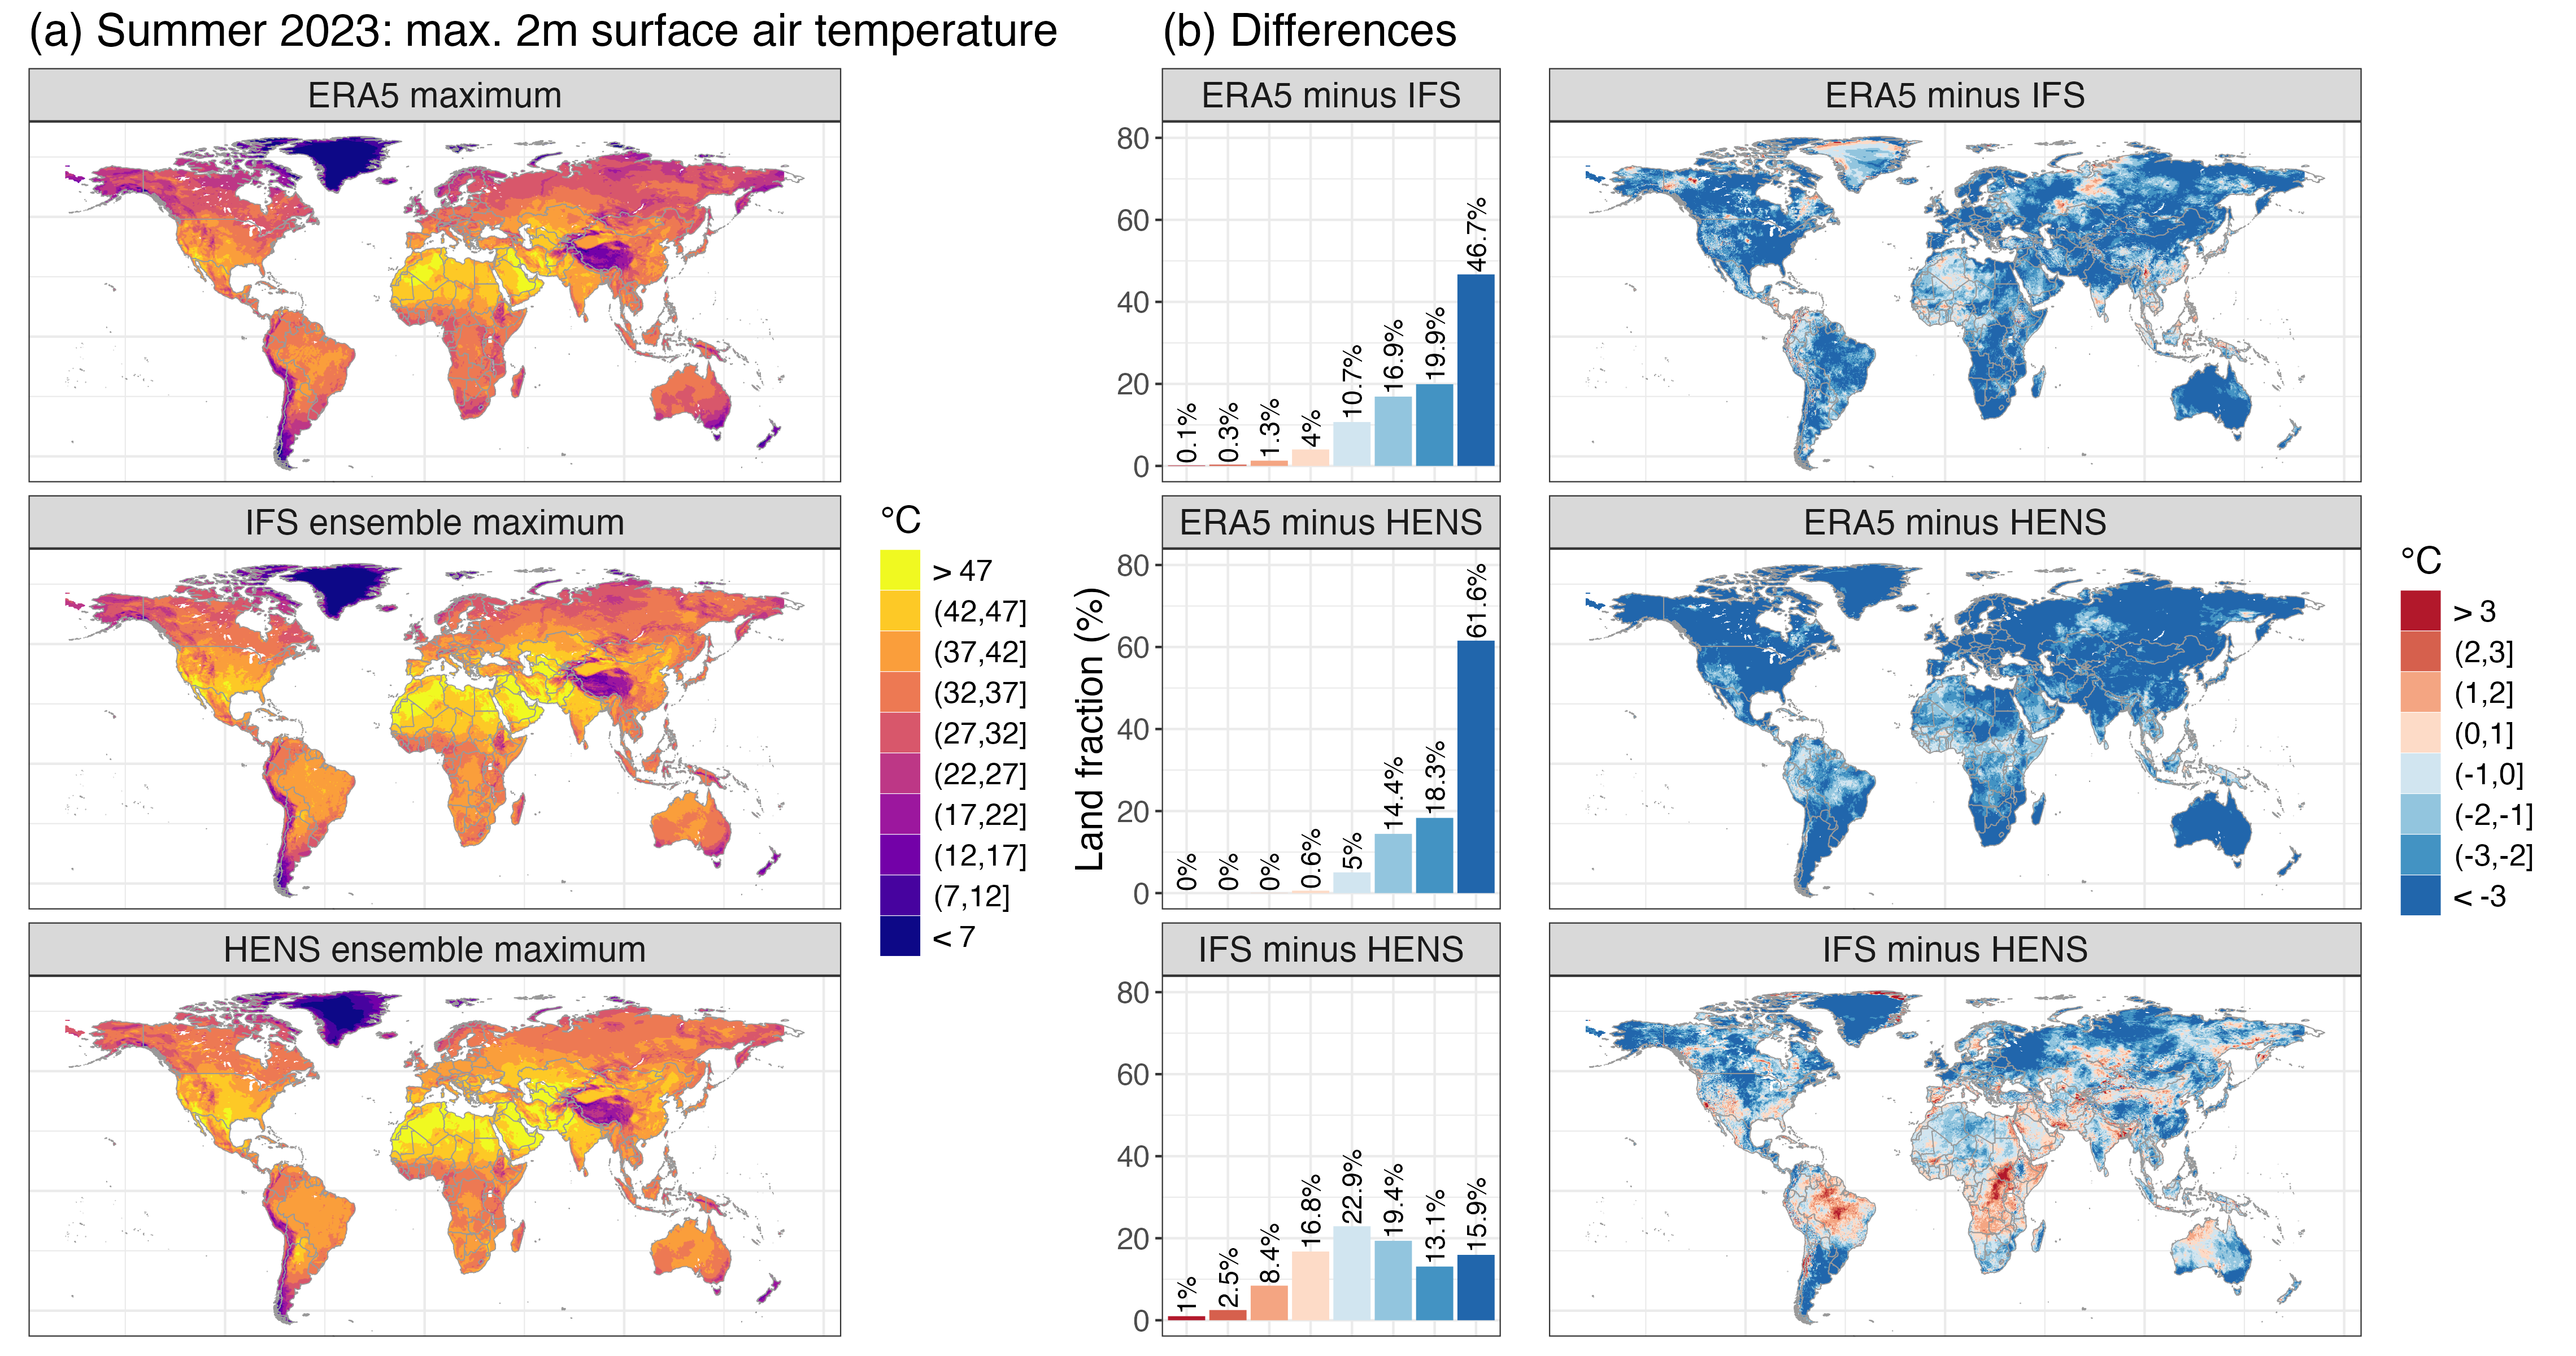
\includegraphics[width = \textwidth]{Figure_t2m_maxima_diff.png}
\caption{Comparison of three different versions of the hottest 2-meter air temperatures over global land regions from 01 June 2023 to 31 August 2023. Panel (a) shows the hottest temperatures from ERA5 (our best reconstructions of the realized temperatures; left), the IFS forecast ensemble (middle), and the HENS ensemble (right). Panel (b) compares the differences between three versions of reality.}
\label{fig:threeversions}
\end{figure*}

Next, Figure~\ref{fig:threeversions}(b) presents a comparison of the 2m temperature extremes in each of the data sources. For more than 94\% of the global land area considered, the IFS ensemble maximum is larger than the realized ERA5 maximum; for nearly half of the globe, the IFS values are more than $3^\circ$C warmer than ERA5. For the other 5.8\%, the ERA5 maximum was, on average, $0.8^\circ$C warmer (and at most $6.3^\circ$C). The HENS ensemble maxima are almost uniformly larger than the ERA5 maxima (99\% of the land areas considered), while for the other 1\% the ERA5 maximum was, on average, $0.48^\circ$C warmer (and at most $3.5^\circ$C). While both forecast ensembles contain the ERA5 surface temperature extremes for large fractions of the globe, a direct comparison of the IFS and HENS ensembles is more nuanced. For most of the global land areas considered (71.2\%), the HENS ensemble maxima are larger than the IFS ensemble maxima. In some cases, this exceedance is considerable: more than $3^\circ$C in Greenland, northern Asia, Northern Europe, Alaska, and Argentina. However, for 28\% of the land areas considered the IFS ensemble maxima are warmer than those in HENS: on average, about $1.1^\circ$C warmer and, in spatially isolated areas, as much as $17.3^\circ$C warmer. 

Clearly, the 2m temperature extremes generated by a huge ML-based ensemble can exceed both observed temperatures and those generated by a traditional numerical weather prediction ensemble. The spatial distribution and magnitude of these exceedances provide important information about where else might have experienced an extreme heatwave. We also find that the much larger ML-based ensemble maxima dominate the IFS ensemble maxima for much of the globe, but there remain some regions, mostly in the southern Hemisphere, for which the IFS ensemble was warmer than HENS. Further research is necessary to understand why the IFS ensemble exceeds HENS in these regions and whether this is due to a model bias in HENS.

% In almost all cases, the IFS ensemble max is larger than the ERA5 max (93.4\% of grid boxes)
% For the other 6.6\%, the ERA5 max was on average 0.94C warmer (at most 7.98C)
% In nearly all cases, the HENS ensemble max is larger than the ERA5 max (99.2\% of grid boxes)
% For the other 0.8\%, the ERA5 max was on average 0.48C warmer (at most 3.48C)
% The HENS ensemble max is larger than the IFS ensemble max for 75.6\% of grid boxes
% For the other 24.4\%, the IFS ensemble max was on average 1.10C warmer (at most 17.24C)


\subsection{Probabilistic comparison of IFS-GEV statistics and HENS} \label{subsec:probcomp}

% \begin{figure*}[!t]
% \centering
% \includegraphics[width = \textwidth]{Figure_IFS_GEV_probContain_HENS_deltaT.jpg}
% \caption{(OLD) Comparison of IFS-GEV extreme event thresholds ($99.9\%$ percentile) with corresponding empirical estimates calculated from the HENS ensemble. Panel (a) tallies the probability that the IFS-GEV threshold contains (is larger than) the HENS threshold; lighter colors indicate that HENS values are more extreme than IFS-GEV. Panel (b) tallies the difference in the IFS-GEV event threshold (the posterior median) and the HENS estimate. Panel insets show the land fraction in each color category.}
% \label{fig:probcontain}
% \end{figure*}

One downside of comparing ensemble maxima as in Figure~\ref{fig:threeversions} is that the results are highly sensitive to individual ensemble members. Furthermore, in Figure~\ref{fig:threeversions}, the IFS maxima are disadvantaged purely from the standpoint that the HENS ensemble is two orders of magnitude larger.
However, since we have access to extreme value theory tools via the GEV distribution, for the IFS ensemble we can extrapolate beyond the ensemble maximum. We refer to these estimates as ``IFS-GEV.'' The IFS-GEV allows us to extrapolate the IFS ensemble to extreme thresholds or percentiles larger than $100(1-1/50)\% = 98\%$ (the ensemble maximum).
% , e.g., $r$-day events or return levels (the $1-1/r$ quantile) for $r \in\{100, 1000, 2000, 5000, \infty\}$. Here, the ``$\infty$ return level'' is the upper bound of the GEV distribution. 
Note that we can calculate much more extreme thresholds from the HENS ensemble empirically (up to $100(1-1/7424)\% \approx 99.986\%$), without fitting GEV distributions, given the huge number of ensemble members. Here and throughout, we use the $99.9\%$ percentile as the extreme threshold of interest since this threshold from HENS contains the ERA5 t2m maxima for nearly 98\% of the global land area considered (and there are diminishing returns on the fraction of containment for higher percentiles; see Table S2 in the Supporting Information).

However, since the IFS-GEV extreme thresholds are statistical estimates based on a finite amount of data, we must account for their uncertainty which, in a Bayesian framework, can be quantified using the posterior distribution. To compare a single number (the HENS extreme threshold) with a statistical estimate (the IFS-GEV extreme threshold), we calculate the posterior probability that the HENS threshold is contained by the IFS-GEV threshold. For easier interpretation, we convert these probabilities to categories inspired by the IPCC confidence language \citep{mastrandrea2010guidance}; see also \cite{Risser2025data}. The categories are shown in the legend of Figure~\ref{fig:probcontain}(a). We also calculate differences between the best estimate of the IFS-GEV threshold (the posterior median) and the HENS threshold.

\begin{figure*}[!t]
\centering
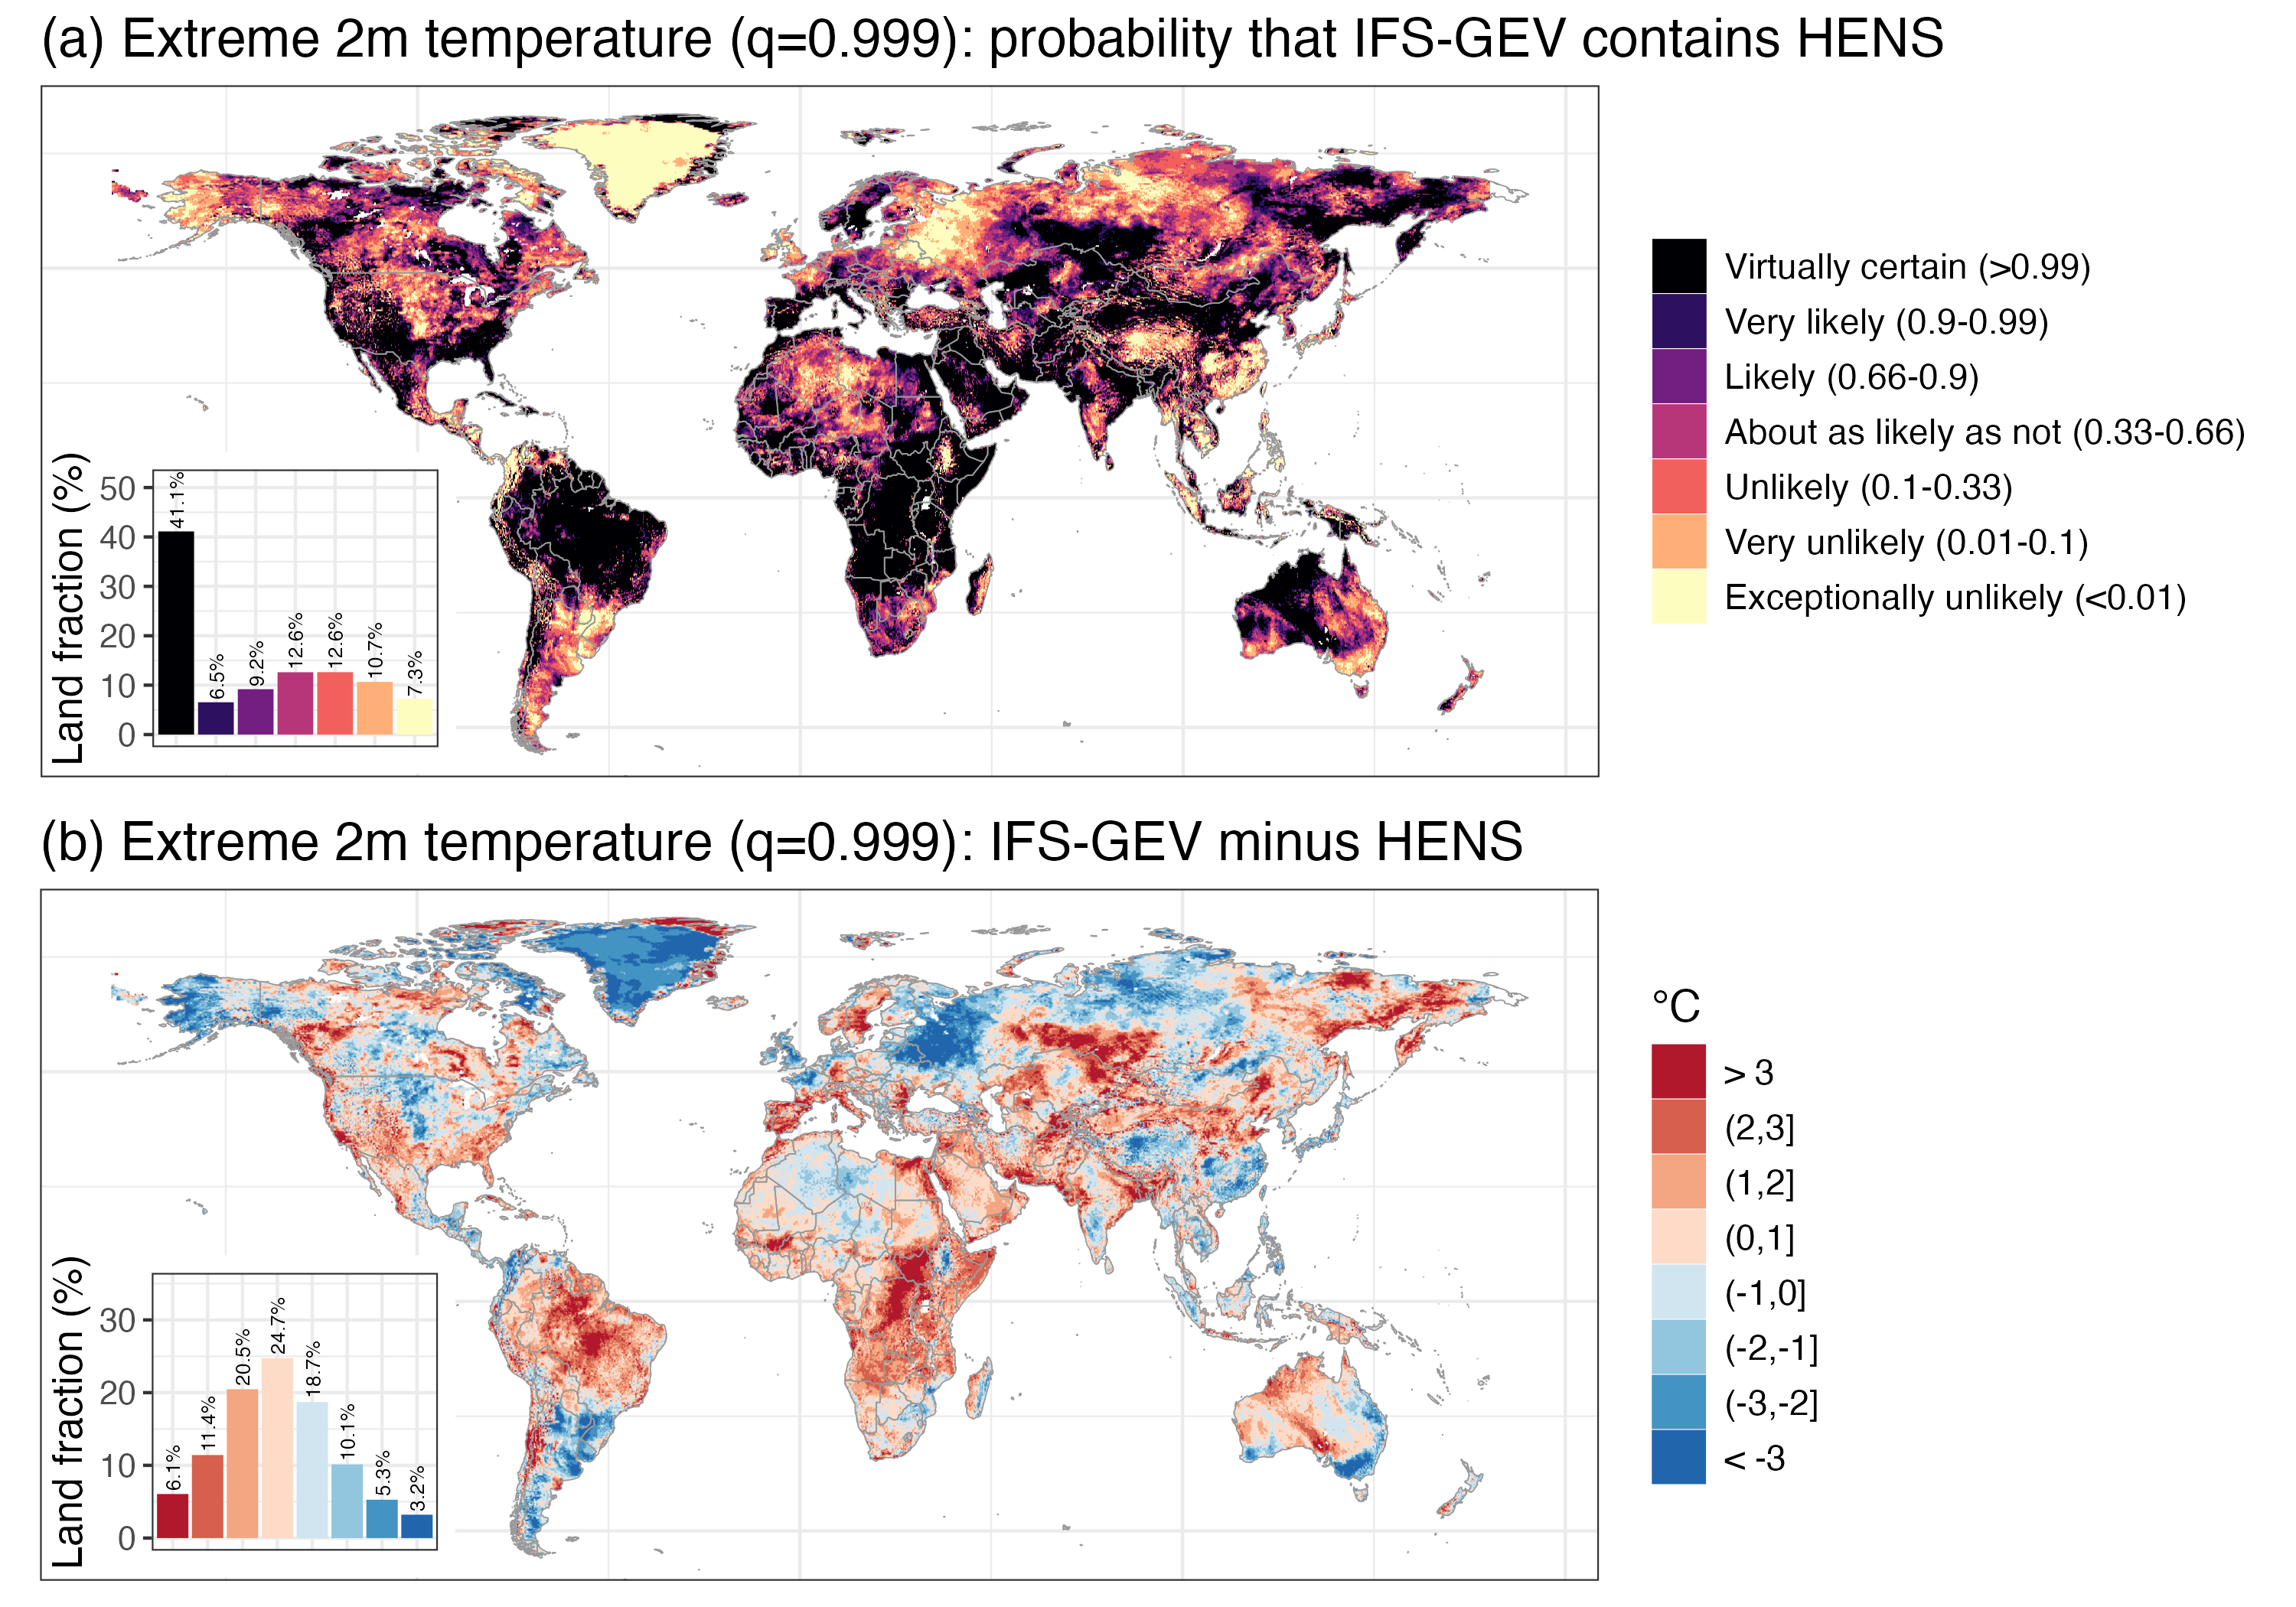
\includegraphics[width = \textwidth]{Figure_t2m_probContain_1000day.png}
\caption{Comparison of IFS-GEV extreme event thresholds for 2m temperature ($99.9\%$ percentile) with corresponding empirical estimates calculated from the HENS ensemble. Panel (a) tallies the probability that the IFS-GEV threshold contains (is larger than) the HENS threshold; lighter colors indicate that HENS values are more extreme than IFS-GEV. Panel (b) tallies the difference in IFS-GEV event threshold (posterior median) and the HENS estimate. Panel insets show the land fraction in each category.}
\label{fig:probcontain}
\end{figure*}


Figure~\ref{fig:probcontain} shows results for the extreme threshold of interest. In Figure~\ref{fig:probcontain}(a), we tally the posterior probability that the IFS-GEV extreme threshold contains the corresponding HENS quantity. Here, lighter colors indicate that HENS values are more extreme than what would have been expected using only the IFS-GEV analysis. Even though the HENS ensemble maxima are often larger than the IFS ensemble maxima (for approximately 70\% of the area considered; bottom panel of Figure~\ref{fig:threeversions}b.), we are \textit{virtually certain} that the IFS-GEV threshold contains the HENS threshold for more than one-third of the land area considered in this analysis. For another one-third, % ($6.5\%+9.2\%+12.6\%=28.3\%$),
the HENS threshold is (at least) \textit{about as likely as not} to be contained by the IFS-GEV quantity. For the final 30.6\% of the land area considered here, the HENS extreme thresholds are definitively extreme compared to the IFS-GEV, and for 7.3\% of the land area the HENS estimates are \textit{exceptionally unlikely} even relative to extrapolating beyond the IFS ensemble via GEV tools. These \textit{exceptionally unlikely} temperatures occur primarily in the northern high latitudes: the majority of Greenland, large portions of eastern and northern Russia, and Alaska. However, \textit{exceptionally unlikely} temperatures in HENS (relative to IFS-GEV) also occur in eastern China, northern Africa, and parts of the central United States and Canada. 
% Unsurprisingly, places where the IFS-GEV threshold is larger than the HENS quantity (shown in Figure~\ref{fig:threeversions}b.) align with geospatial locations where the HENS estimates are \textit{virtually certain} contained.
When the HENS extreme threshold is larger than the IFS-GEV quantity (blue colors in Figure~\ref{fig:probcontain}b.), the exceedance is most often on the order of $1$-$3^\circ$C and occasionally larger than $3^\circ$C. Analysis of gauged temperature records verifies that HENS is generating realistic high-latitude temperatures in places like Greenland (see Section 2 of the Supporting Information). We note that these results are insensitive to the specific extreme threshold used; see Figure S3.

% Lastly, we note that these results are insensitive to the specific extreme threshold shown in Figure~\ref{fig:probcontain}: the results are largely similar whether we consider the 99\%, 99.95\%, or 99.98\% percentiles, instead of the maximum. Figure~\ref{fig:barchart} tallies the land fraction that falls into each containment and difference category across these other extreme thresholds. Interestingly, the fraction of HENS estimates that are ``virtually certain'' according to IFS-GEV decreases as we consider more and more extreme thresholds; similarly, the distribution of the differences between HENS and IFS-GEV shifts to more negative values for more extreme events.
% The only striking difference is in the tallying of IFS-GEV upper bounds minus the HENS ensemble maxima (rightmost panel of Figure~\ref{fig:barchart}b.), where the IFS-GEV upper bound is more than $3.5^\circ$C larger than the HENS maxima for nearly one-quarter of the global land area. 
% We hypothesize that this is due to the increased statistical noise associated with the 99.98\% percentile relative to, e.g., the 99\% percentile, since at these levels we are extrapolating further and further beyond the range of the 50 IFS ensemble members.
% upper bound relative to, e.g., the 5000-day return level.  
% Spatial patterns of containment probabilities and differences for these other levels of extremity are similar to Figure~\ref{fig:probcontain} and are omitted for brevity.
% shown in Supplemental Figures~\ref{supp:fig:probcontain} and \ref{supp:fig:diff}: aside from the upper bounds (which again exhibit more statistical noise), the spatial patterns are largely consistent regardless of the specific return level considered. 

In summary, extrapolation of the IFS ensemble using GEV theory allows us to anticipate many more of the extreme six-hourly surface temperatures generated by HENS: the HENS extreme thresholds are (at least) \textit{about as likely as not} to be contained for more than two-thirds of the global land areas considered. However, for the other one-third, the HENS estimates are (at best) \textit{unlikely} and, for 7.3\% of the land areas considered, \textit{exceptionally unlikely}. Once again, the spatial distribution and relative magnitude of the \textit{exceptionally unlikely} HENS extreme temperatures provides important information on locations that could have experienced even more extreme heatwaves. 

\subsection{Heat index storylines}

While we have thus far focused on dry heat extremes by looking at 2m temperatures, the ML ensemble also allows us to assess humid heat extremes as characterized by the heat index \citep{Lu2022}. The heat index accounts for the impacts of humidity and temperature on heat stress for humans \citep{Lu2023}, and extreme heat index values are often associated with higher mortality rates \citep{Wehner2017}. As we found for 2m temperature (Sections~\ref{subsec:threeversions} and \ref{subsec:probcomp}), the huge ML ensemble produces heat indices that exceed both observations and a traditional NWP ensemble (Supplemental Figure S6) and are unusual even relative to extrapolation of heat index values from the IFS ensemble using GEV theory (see Supplemental Figure S7). 

Compared to the IFS, the massive sample size of HENS provides significant value in quantifying heat index extremes for regions prone to high humidity. Comparing the bottom rights panels of Figures~\ref{fig:threeversions} and S6, HENS captures more extreme humid-heat events in the Southeastern United States, where moisture transport from the Gulf of Mexico frequently triggers intense heatwaves \citep{Algarra2019, Milrad2025}. Similarly, HENS identifies more severe humid extremes in India near the Bay of Bengal and the Arabian Sea, regions where monsoon depressions drive dangerous conditions. In contrast, HENS 2m temperature data shows a greater range of extremes in the Central United States, where dry heatwaves, in part driven by soil moisture deficits, dominate.

To demonstrate how the ML ensemble forecasts humid heat risks, we used HENS to develop ``heat index storylines" for every location globally.  We define the ``HENS Storyline'' as the 99.9th percentile of the maximum summertime temperature from each HENS member.  As it is a storyline simulation, this quantity does not correspond to a specific probability or a return level: rather, we use it as a benchmark for the summertime maximum to guide stakeholder extremes preparedness \citep{Shepherd2018}.  HENS yields 7,424 plausible versions of summer 2023, and the HENS Storyline is a method to quantify the different way the temperatures could plausibly evolve.
Despite the fact that the heat index is a heavier-tailed phenomena than 2m temperatures (Supplemental Figure S2), the HENS heat index values are more highly unusual than IFS-GEV in comparison to 2m temperature extremes (Supplemental Figure S3). For example, the HENS storyline of the heat index exceeds the IFS-GEV quantity by more than 2$^\circ$C for nearly 15\% of the globe (compared to just 8.5\% for 2m temperatures).  Additionally, for approximately, 42\% of the globe, the HENS Storyline is \textit{unlikely}, \textit{very unlikely}, or \textit{exceptionally unlikely} to have occurred according to the IFS-GEV quantity.  This underscores the utility of running huge ensembles to quantify and prepare for worst-case extremes, compared to running smaller ensembles like IFS.

%TODO: Make a plot that shows the 2D distribution of all unlikely summertime max values, where unlikely is defined by the IFS value.  The X axis is IFS GEV upper bound (or maybe ERA5).  Y axis is HENS storyline.

\begin{figure}
    \centering
    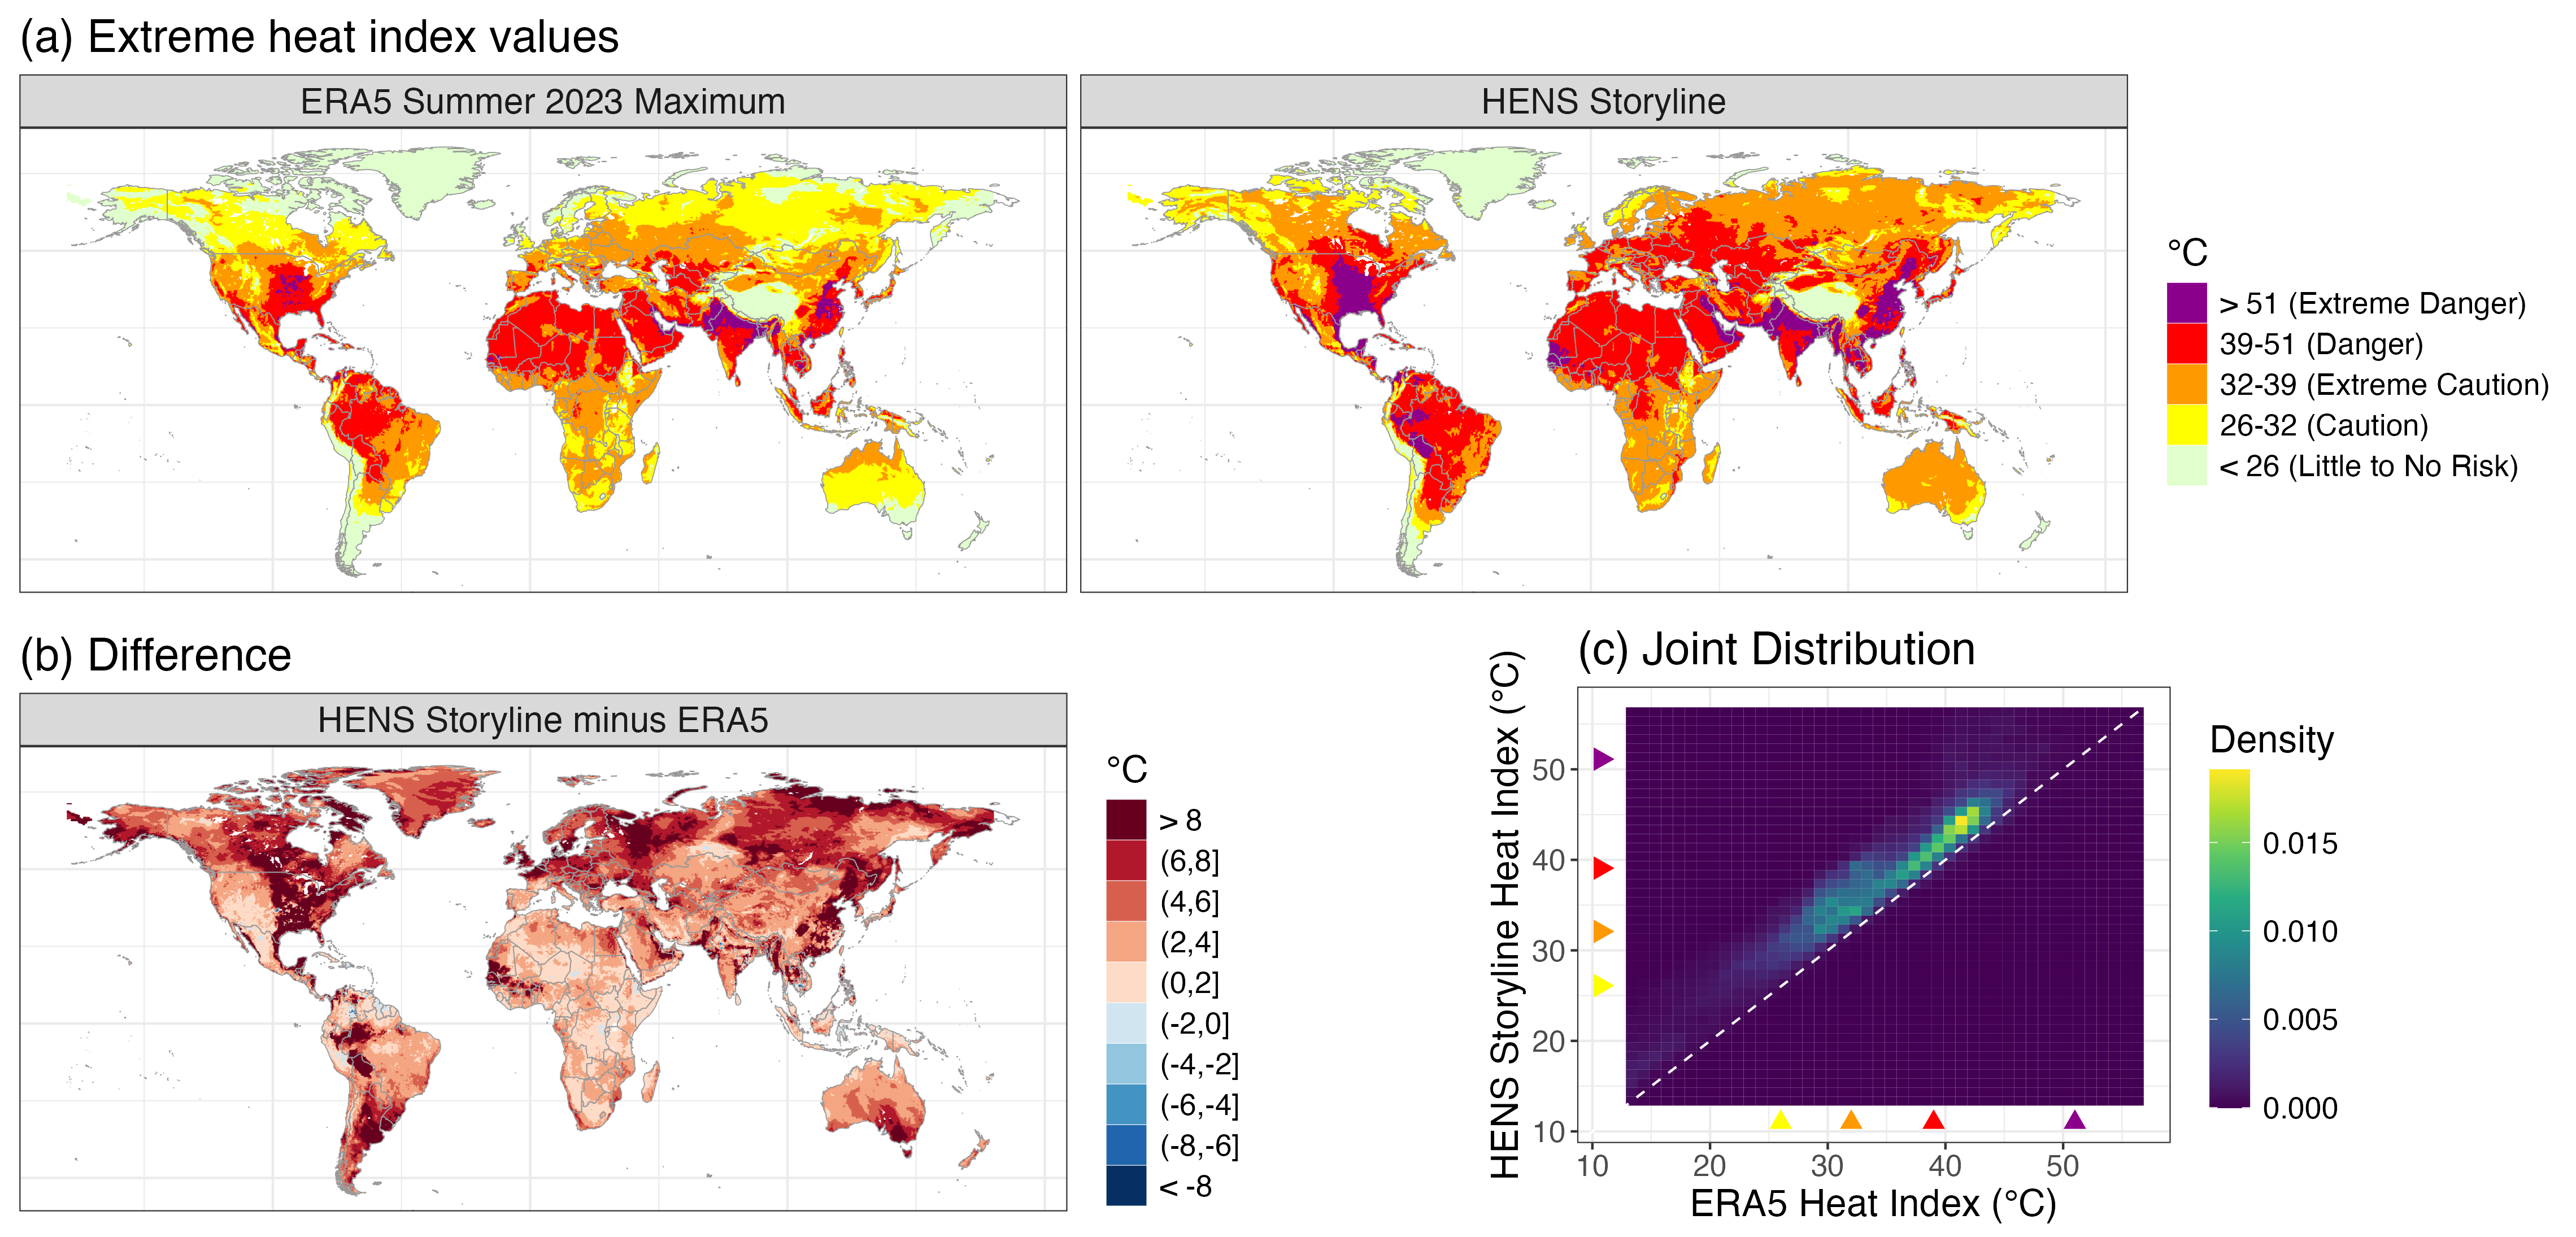
\includegraphics[width=\linewidth]{four_panel_heatindex_mark.png}
    \caption{{Extreme heat index analysis for summer 2023.} Panel (a) shows the summer max heat index from ERA5 (left) and the storyline (the 99.9th percentile) of the HENS 10-day simulations (right).  Panel (b) shows the difference, HENS minus ERA5.  Panel (c) shows the joint distribution of all events where IFS-GEV is unlikely, very unlikely, or exceptionally unlikely to contain the HENS extreme (Figure S7a).  The histogram in (c) is shown for all land grid cells and weighted by latitude.  Panels (a) and (c) mark the National Weather Service public safety thresholds for 
    caution (26$^\circ$C), extreme caution (32$^\circ$C), danger (39$^\circ$C), and extreme danger (51$^\circ$C).
    % caution (299K), extreme caution (305K), danger (312K), and extreme danger (324K).
    }
    \label{fig:four_panel_heat_index}
\end{figure}

Figure~\ref{fig:four_panel_heat_index} compares the observed 2023 maximum heat index from ERA5 to the HENS storyline, binned by National Weather Service (NWS) public safety levels. The NWS classifies heat risk into four categories: Caution, Extreme Caution, Danger, and Extreme Danger. While regional thresholds vary, these categories correspond to approximately 26$^\circ$C (80$^\circ$F), 32$^\circ$C (90$^\circ$F), 39$^\circ$C (103$^\circ$F), and 51$^\circ$C (125$^\circ$F),
% 299 K, 305 K, 312 K, and 324 K,
respectively. In Figure~\ref{fig:four_panel_heat_index}, we map the maximum values from both ERA5 and the HENS storyline into these four classifications. 
% To assess direct physiological outcomes, we used the heat index to calculate excess skin blood flow \citep{Lu2023}. This metric provides a key advantage for evaluating the impact of humid heat extremes, as it quantifies the net physiological strain more accurately than temperature alone \citep{Romps2022}.
Figure~\ref{fig:four_panel_heat_index}(a) shows that the Midwest and Southeastern U.S. would have experienced substantially larger areas under Extreme Danger alerts in the HENS storyline compared to ERA5. Similarly, large portions of Central Europe shift into a higher risk category, moving from Extreme Caution in ERA5 to Danger in HENS. In these regions, the HENS storyline produces heat indices 5–10$^\circ$C higher than the ERA5 summertime maxima (Figure~\ref{fig:four_panel_heat_index}b). In contrast, the Southwestern U.S. shows relatively small increases. This reflects the region’s arid climate, which limits the humidity contribution to the heat index, as well as the fact that the region experienced severe summer heatwaves in ERA5 \citep{Lopez2025}. Consistent with this, the increase in 2m air temperature between IFS and HENS is also smaller in this region (Figure~\ref{fig:threeversions}).

Finally, we examine the events that are missed by IFS-GEV by focusing on locations where IFS-GEV assigns a low probability (less than 33\% in Figure S7) of containing the HENS maximum. Figure~\ref{fig:four_panel_heat_index}(c) shows the joint distribution across all land grid cells of the ERA5 summertime maximum and the corresponding HENS storyline. These cases are particularly important because they represent situations in which the traditional ensemble framework underestimates the actual realized severity of extremes relative to the much larger HENS ensemble.
% In addition to the NWS threshlds, we also use the heat index to calculate quantities more directly relelevant to direct physiological outcomes \citep{Lu2023}.  In Figure~\ref{fig:era5_vs_hens_blood_flow}, we use the heat index to calculate excess blood flow.  Excess skin blood flow is a key benefit of using the heat index model to assess the physiological impact of humid heat extremes, and this metric has been used to show the net benefit of correctly calculating the heat index \citep{Romps2022}
For more than 98\% of these cases, the HENS Storyline is larger than the realized ERA5 maximum by an average of 3.9$^\circ$C. In many cases these increased heat index values change the risk category: for example, 14.2\% of these cases shift from ``Extreme Caution'' to ``Danger,'' and 3.2\% shift from ``Danger'' to ``Extreme Danger.'' The implication is that traditional ensemble forecasts can, in some cases, substantially underestimate the realized extreme heat risk. As with 2m temperature, the huge ML ensemble provides more refined sampling of the upper tail of the heat index and a better characterization of the full range of plausible outcomes.

\section{Discussion} \label{sec:Discussion}

In this work, we show that a 7,424-member huge ensemble captures the long upper tails of weather hazards that traditional 50-member NWP ensembles miss. With this petabyte-scale ensemble, we characterize plausible extreme weather events that could have occurred during summer 2023, the hottest summer on record at the time. As summers reaching 2023 levels become increasingly likely due to climate change, the ability to fully characterize the envelope of possible low-likelihood, high impact heat extremes will only grow in importance.

A key emergent property of HENS is that its simulated maxima often exceed the data-driven upper bounds predicted by the IFS-GEV distribution. If HENS were merely sampling further into the existing IFS tail, its results would remain within the GEV envelope. Instead, for both the 2m air temperature and heat index, we find that the global land surface partitions into three roughly equal regimes: regions where HENS maxima fall well within the GEV upper bounds derived from IFS, regions where HENS maxima are comparable to those bounds, and regions where HENS maxima exceed the GEV-implied threshold entirely. This three-way partition is not prescribed by theory and represents an emergent property of HENS. This behavior indicates that HENS is not merely resampling the IFS tail.  Instead, it is generating extreme weather states that are unexplored by the IFS ensemble's sample of summer 2023 internal variability. Ultimately, HENS reveals an envelope of plausible meteorological extremes that traditional extreme value theory and smaller ensembles fail to capture.

% Our results also demonstrate the utility of huge ML forecast ensembles for quantifying and simulating storyline simulations of the most extreme events.
More broadly, this work establishes a new approach for conducting storyline simulations targeting novel classes of extremes and compound hazards.
A current major barrier to storyline simulations is that existing methods demand significant programmer expertise and computational resources, limiting their application in regions that lack access to both. Machine learning weather models offer a turnkey solution, enabling global storyline simulations without the infrastructure and specialized knowledge required by conventional approaches. For example, a single 15-day forecast from the ML model takes approximately one minute, which is many orders of magnitude faster than comparable numerical simulations \citep{Mahesh2024hugeensemblesidesign}. Furthermore, forecasts can be easily initialized from publicly available reanalysis data sets such as ERA5. This democratization of tools and models for constructing storyline simulations presents an important opportunity for their broad and systematic application for extreme events in all corners of the globe.

% Future work should assess the human health impacts of these heat extremes at higher resolution, particularly over densely populated regions. Additionally, this study focuses on moist heat extremes, but the HENS framework is equally applicable to dry heat extremes, which carry important implications for wildfire risk. More broadly, this work establishes a new approach for conducting storyline simulations targeting novel classes of extremes and compound hazards. \todo{AM 3/16 - should we add a sentence here about ML emulators and gray swans (with respect to Pedram's paper?)}






% \section{Conclusions}


%% Enter Figures and Tables near as possible to where they are first mentioned:
%
% DO NOT USE \psfrag or \subfigure commands.
%
% Figure captions go below the figure.
% Acronyms used in figure captions will be spelled out in the final, published version.

% Table titles go above tables;  other caption information
%  should be placed in last line of the table, using
% \multicolumn2l{$^a$ This is a table note.}
% NOTE that there is no difference between table caption and table heading in the final, published version
%
%----------------
% EXAMPLE FIGURES
%
% \begin{figure}
% \includegraphics{example.png}
% \caption{caption}
% \end{figure}
%
% Giving latex a width will help it to scale the figure properly. A simple trick is to use \textwidth. Try this if large figures run off the side of the page.
% \begin{figure}
% \noindent\includegraphics[width=\textwidth]{anothersample.png}
%\caption{caption}
%\label{pngfiguresample}
%\end{figure}
%
%
% If you get an error about an unknown bounding box, try specifying the width and height of the figure with the natwidth and natheight options. This is common when trying to add a PDF figure without pdflatex.
% \begin{figure}
% \noindent\includegraphics[natwidth=800px,natheight=600px]{samplefigure.pdf}
%\caption{caption}
%\label{pdffiguresample}
%\end{figure}
%
%
% PDFLatex does not seem to be able to process EPS figures. You may want to try the epstopdf package.
%

%
% ---------------
% EXAMPLE TABLE
%
% \begin{table}
% \caption{Time of the Transition Between Phase 1 and Phase 2$^{a}$}
% \centering
% \begin{tabular}{l c}
% \hline
%  Run  & Time (min)  \\
% \hline
%   $l1$  & 260   \\
%   $l2$  & 300   \\
%   $l3$  & 340   \\
%   $h1$  & 270   \\
%   $h2$  & 250   \\
%   $h3$  & 380   \\
%   $r1$  & 370   \\
%   $r2$  & 390   \\
% \hline
% \multicolumn{2}{l}{$^{a}$Footnote text here.}
% \end{tabular}
% \end{table}

%%%%%%%%%%%%%%%%%%%%%%%%%%%%%%%%%%%%%%%%%%%%%%%
% SIDEWAYS FIGURES and TABLES
% AGU prefers the use of {sidewaystable} over {landscapetable} as it causes fewer problems.
%
% \begin{sidewaysfigure}
% \includegraphics[width=20pc]{figsamp}
% \caption{caption here}
% \label{newfig}
% \end{sidewaysfigure}
%
%  \begin{sidewaystable}
%  \caption{Caption here}
% \label{tab:signif_gap_clos}
%  \begin{tabular}{ccc}
% one&two&three\\
% four&five&six
%  \end{tabular}
%  \end{sidewaystable}

%% If using numbered lines, please surround equations with \begin{linenomath*}...\end{linenomath*}
%\begin{linenomath*}
%\begin{equation}
%y|{f} \sim g(m, \sigma),
%\end{equation}
%\end{linenomath*}

%%% End of body of article

%%%%%%%%%%%%%%%%%%%%%%%%%%%%%%%%%%%%%%%%%%%%%%%
%% Optional Appendices go here
%
% The \appendix command resets counters and redefines section heads
%
% After typing \appendix
%
%\section{Here Is Appendixf Title}
% will show
% A: Here Is Appendix Title
%
% \newpage
% \appendix

%%%%%%%%%%%%%%%%%%%%%%%%%%%%%%%%%%%%%%%%%%%%%%%
% Optional Glossary, Notation or Acronym section goes here:
%
% Glossary is only allowed in Reviews of Geophysics
%  \begin{glossary}
%  \term{Term}
%   Term Definition here
%  \term{Term}
%   Term Definition here
%  \term{Term}
%   Term Definition here
%  \end{glossary}


%%%%%%%%%%%%%%%%%%%%%%%%%%%%%%%%%%%%%%%%%%%%%%%
% Acronyms
%% NOTE that acronyms in the final published version will be spelled out when used in figure captions.
%   \begin{acronyms}
%   \acro{Acronym}
%   Definition here
%   \acro{EMOS}
%   Ensemble model output statistics
%   \acro{ECMWF}
%   Centre for Medium-Range Weather Forecasts
%   \end{acronyms}


%%%%%%%%%%%%%%%%%%%%%%%%%%%%%%%%%%%%%%%%%%%%%%%
% Notation
%   \begin{notation}
%   \notation{$a+b$} Notation Definition here
%   \notation{$e=mc^2$}
%   Equation in German-born physicist Albert Einstein's theory of special
%  relativity that showed that the increased relativistic mass ($m$) of a
%  body comes from the energy of motion of the body—that is, its kinetic
%  energy ($E$)—divided by the speed of light squared ($c^2$).
%   \end{notation}



%%%%%%%%%%%%%%%%%%%%%%%%%%%%%%%%%%%%%%%%%%%%%%%
%
% DATA SECTION and ACKNOWLEDGMENTS
%
%%%%%%%%%%%%%%%%%%%%%%%%%%%%%%%%%%%%%%%%%%%%%%%

% \newpage %to delete


\section*{Open Research Section}

The HENS code, datasets, and models are all stored at \url{https://doi.org/10.5061/dryad.2rbnzs80n}, via Data Dryad. The code is integrated with Zenodo at the prior DOI. We include the code to train SFNO, conduct ensemble inference with bred vectors and multiple checkpoints, and scoring and analysis code. We also open-source the model weights of the trained SFNO. See the README of the DOI for information on how to use the codebase and for the permissive license associated with the code and data. The code is available via the Lawrence Berkeley National Lab-modified BSD license, and the data is available with a CC0 license. 

% Data from the ECMWF 5th Reanalysis \citep{Hersbach2020} are obtained from 

% \begin{itemize}
%     \item \todo{Fill in these details.} Source of ERA5 data
%     \item Source of ECWMF IFS data
%     % \item Source of Greenland surface met data.


% \end{itemize}

% Required acknowledgements for PROMICE
Data from the Programme for Monitoring of the Greenland Ice Sheet (PROMICE) are provided by the Geological Survey of Denmark and Greenland (GEUS) at \url{http://www.promice.dk}. ZAC, LYN, FRE and \texttt{NUK\_K} stations are financially supported by the Glaciobasis programme as part of the Greenland Ecosystem Monitoring project (\url{https://g-e-m.dk/}). The \texttt{NUK\_K} station is owned and maintained by Asiaq Greenland Survey. The WEG stations are funded and maintained by Jakob Abermann at the Department of Geography and Regional Science of the University of Graz. The \texttt{RED\_L} station is funded and maintained by Rainer Prinz at the Department of Atmospheric and Cryospheric Sciences of the University of Innsbruck. The \texttt{NUK\_B} station is funded and maintained by James Lea at the University of Liverpool. The \texttt{SER\_B} station is funded and maintained by Anders Bjørk at the Department of Geosciences and Natural Resource Management of the University of Copenhagen.
% There are four key components for the code and data used in this manuscript.  
% For reproducibility, the training code for FourCastNet, and the TCs from summer 2023 within the HENS dataset are stored with Zenodo DOIs at the following links, respectively: \url{https://zenodo.org/records/13137296} and \url{https://zenodo.org/records/14939820}.

% \begin{itemize}
%     \item Trained FourCastNet Models: We release the trained model weights via this portal. Each of the models uses a different Pytorch seed for weight initialization, that is reflected by "seed[SEED]" in the model name. For each of the SFNO checkpoints there is config.json file with the description of training parameters.

%     \item Ensemble Inference with FourCastNet Models: Ensemble inference can be performed with the repository NVIDIA earth2mip available at \url{https://github.com/ankurmahesh/earth2mip-fork/tree/HENS}. That version contains bred vectors and ensemble inference. Extra needed files are at \url{https://portal.nersc.gov/cfs/m4416/}.

%     \item  Code for Training FourCastNet Checkpoints: We have used Modulus-Makani v0.1.0 available at \url{https://github.com/NVIDIA/modulus-makani} with a few minor modifications for training on Perlmutter at \url{https://zenodo.org/records/13137296}.

%     \item TempestExtremes for Predicted TCs: We use TempestExtremes at the GitHub repository \url{https://github.com/ClimateGlobalChange/tempestextremes} to identify and track predicted tropical cyclones in HENS ensemble data. Configuration files for running TempestExtremes on HENS are available at \url{https://zenodo.org/records/14939489}. 
% \end{itemize}

% \section*{As Applicable – Inclusion in Global Research Statement}
% The Authorship: Inclusion in Global Research policy aims to promote greater equity and transparency in research collaborations. AGU Publications encourage research collaborations between regions, countries, and communities and expect authors to include their local collaborators as co-authors when they meet the AGU Publications authorship criteria (described here: https://www.agu.org/publications/authors/policies\#authorship). Those who do not meet the criteria should be included in the Acknowledgement section. We encourage researchers to consider recommendations from The TRUST CODE - A Global Code of Conduct for Equitable Research Partnerships (https://www.globalcodeofconduct.org/) when conducting and reporting their research, as applicable, and encourage authors to include a disclosure statement pertaining to the ethical and scientific considerations of their research collaborations in an “Inclusion in Global Research Statement’ as a standalone section in the manuscript following the Conclusions section. This can include disclosure of permits, authorizations, permissions and/or any formal agreements with local communities or other authorities, additional acknowledgements of local help received, and/or description of end-users of the research. You can learn more about the policy in this editorial. Example statements can be found in the following published papers: 
% Holt et al. (https://agupubs.onlinelibrary.wiley.com/doi/full/10.1029/2022JG007188), 
% Sánchez-Gutiérrez et al. (https://agupubs.onlinelibrary.wiley.com/doi/abs/10.1029/2023JG007554), 
% Tully et al. (https://agupubs.onlinelibrary.wiley.com/doi/epdf/10.1029/2022JG007128) 
% Please note that these statements are titled as “Global Research Collaboration Statements” from a previous pilot requirement in JGR Biogeosciences. The pilot has ended and statements should now be titled “Inclusion in Global Research Statement”.



\acknowledgments

This research was supported by the Director, Office of Science, Office of Biological and Environmental Research of the U.S. Department of Energy under Contract No. DE-AC02-05CH11231 and by the Regional and Global Model Analysis Program area within the Earth and Environmental Systems Modeling Program (MDR, JSN, WDC, AM). The research used resources of the National Energy Research Scientific Computing Center (NERSC), also supported by the Office of Science of the U.S. Department of Energy, under Contract No. DE-AC02-05CH11231. The computation for this paper was supported in part by the DOE Advanced Scientific Computing Research (ASCR) Leadership Computing Challenge (ALCC) 2023-2024 award ‘Huge Ensembles of Weather Extremes using the Fourier Forecasting Neural Network’ to William Collins (LBNL) and the 2024-2025 award ‘Huge Ensembles of Weather Extremes using the Fourier Forecasting Neural Network’ to William Collins (LBNL).


%%%%%%%%%%%%%%%%%%%%%%%%%%%%%%%%%%%%%%%%%%%%%%%
% REFERENCES and BIBLIOGRAPHY
%
% \bibliography{<name of your .bib file>} don't specify the file extension
% don't specify bibliographystyle
%
%%%%%%%%%%%%%%%%%%%%%%%%%%%%%%%%%%%%%%%%%%%%%%%

\bibliography{agusample}



%Reference citation instructions and examples:
%
% Please use ONLY \cite and \citeA for reference citations.
% \cite for parenthetical references
% ...as shown in recent studies (Simpson et al., 2019)
% \citeA for in-text citations
% ...Simpson et al. (2019) have shown...
%
%
%...as shown by \citeA{jskilby}.
%...as shown by \citeA{lewin76}, \citeA{carson86}, \citeA{bartoldy02}, and \citeA{rinaldi03}.
%...has been shown \cite{jskilbye}.
%...has been shown \cite{lewin76,carson86,bartoldy02,rinaldi03}.
%... \cite <i.e.>[]{lewin76,carson86,bartoldy02,rinaldi03}.
%...has been shown by \cite <e.g.,>[and others]{lewin76}.
%
% apacite uses < > for prenotes and [ ] for postnotes
% DO NOT use other cite commands (e.g., \citet, \citep, \citeyear, \nocite, \citealp, etc.).
%


% % \clearpage
% \begin{appendix}
% \renewcommand{\thefigure}{S\arabic{figure}}
% \renewcommand{\thetable}{S\arabic{table}}
% \renewcommand{\theequation}{S\arabic{equation}}

% \section{Statistical methods} \label{appdx:statmethods}


% \subsection{Extreme value analysis} \label{sec_eva}

% As described in Section~\ref{sec:goals_data}, the focus of our analysis are on 2m temperature and heat index values from the 240, 246, 252, and 258 hour lead times (approximately day 10 of each forecast) across all initialization days. Let $X^{ij}_{dl}$ denote the variable of interest for grid box $\{\bg_i: i=1,\dots,N_\text{grid}\}$, ensemble member $j=1, \dots, N_\text{ens}$, initalization date $d = 1, \dots, 92$, and lead time $l \in \{240, 246, 252, 258\}$. Then, we define $Y_{ij} = \max_{d} \max_{l} X^{ij}_{dl}$. % denote the extreme six-hourly measurements for grid box $\{\bg_i: i=1,\dots,N_\text{grid}\}$ and ensemble member $j=1, \dots, N_\text{ens}$. 
% Since the $\{Y_{ij}\}$ arise as the maximum of a stochastic process over a specified time interval or ``block,'' Theorem~3.1.1 of \cite{Coles2001} states that the cumulative distribution function (CDF) of $Y_{ij}$ can be well approximated by a member of the Generalized Extreme Value (GEV) family of distributions,
% \begin{equation} \label{gev_fam}
% F_i(y) \equiv \mathbb{P}(Y_{ij} \leq y) = \exp\left\{-\left[ 1 + \xi_i\left(\frac{y - \mu_i}{\sigma_i}\right) \right]^{-1/\xi_i} \right\}, \hskip1ex \forall \hskip1ex y \hskip1ex \text{s.t.} \hskip1ex 1 + \xi_i(y - \mu_i)/\sigma_i > 0,
% \end{equation}
% so long as number of the number of measurements per block is large enough (which can be reasonably assumed from the $92\times4=368$ six-hourly periods). The GEV family of distributions~(\ref{gev_fam}) is characterized by three statistical parameters, each of which is grid box-specific: the location parameter $\mu_i \in \mathcal{R}${, }which describes the center of the distribution{;} the scale parameter $\sigma_i>0$, which describes the spread of the distribution{;} and the shape parameter $\xi_i \in \mathcal{R}$. The shape parameter $\xi_i$ is the most important {for} determining the qualitative behavior of the distribution of extreme temperatures: if $\xi_i<0$, the distribution has a finite upper bound and no lower limit; if $\xi_i >0$, the distribution has a finite lower bound and no upper limit; {and} if $\xi_i = 0$, the distribution is again unbounded and the CDF~(\ref{gev_fam}) is interpreted as the limit as the shape parameter $\xi_i$ approaches zero \citep{Coles2001}.

% For the purposes of this analysis, we are interested in a statistical summary of the fitted GEV distribution, namely percentiles or extreme thresholds. These are typically referred to as ``return levels''; however, in the context of this paper we instead use ``extreme thresholds'' since they are calculated from highly conditional data that has been initialized with the large scale conditions present in the summer of 2023. Extreme thresholds for a quantile $q \in (0,1)$ (or percentile $p = 100q \%$) can be calculated based on the statistical parameters of the GEV distribution:
% \begin{equation} \label{eq:returnVal}
%     \phi_{i}(q) = \left\{ \begin{array}{ll}
%     \mu_i - \frac{\sigma_i}{\xi_i}\big[1 - \{-\log q\}^{-\xi_i}\big],  & \xi_i \neq 0 \\[1ex]
%     \mu_i - \sigma_i \log\{-\log q\},  & \xi_i = 0
%     \end{array} \right. 
% \end{equation}
% \citep{Coles2001}. 

% % For the purposes of this analysis, we are interested in two statistical summaries of the fitted GEV distribution:
% % \begin{enumerate}
% %     \item Return levels (sometimes referred to as a return values): six-hourly temperature thresholds for what is considered an extreme or severe temperature at a given location. Return levels are defined for a particular ``return period'' $r$, where often $r = 10, 20, 50,$ or $100$ years, which specifies the event rarity: for example, in any given year, the probability of exceeding the threshold defined by the 20-year return level is $1/20 = 0.05$. Return levels can be calculated based on the statistical parameters of the GEV distribution:
% %     \begin{equation} \label{eq:returnVal}
% %     \phi_{i}(r) = \left\{ \begin{array}{ll}
% %     \mu_i - \frac{\sigma_i}{\xi_i}\big[1 - \{-\log(1-1/r)\}^{-\xi_i}\big],  & \xi_i \neq 0 \\[1ex]
% %     \mu_i - \sigma_i \log\{-\log(1-1/r)\},  & \xi_i = 0
% %     \end{array} \right. 
% %     \end{equation}
% %     \citep{Coles2001}.

% %     \item Data-driven upper bounds: $b_i = \mu_i - {\sigma_i}/{\xi_i}$. This quantity is well-defined when $\xi_i<0$ (as is often the case for extreme temperature). 
% %     Note that the estimated upper bound will always be larger than the largest $\{Y_{ij}\}$.

% % \end{enumerate}

% \subsection{Global analysis} \label{sec_global}

% While Section~\ref{sec_eva} describes an approach for statistical modeling of extreme temperatures, we now turn to inference and uncertainty quantification for the GEV parameters at each grid box. Throughout, we take a Bayesian perspective, since this provides a flexible and straightforward approach for quantifying uncertainty in nonlinear functions of the GEV parameters, e.g., extreme thresholds.
% % We furthermore use a geospatial analysis that accounts for the innate spatial coherence or dependence in the climatology (i.e., nearby grid boxes will experience similar types of heatwaves) of heatwaves. \cite{Zhang_2024} and \cite{Risser2025data} demonstrated the importance of accounting for this dependence when extrapolating well beyond the range of data (i.e., estimating the $99.9\%$ percentile from 50 data points). We now outline an approach to statistically modeling climatological dependence following \cite{cooley2007bayesian} and \cite{Risser2019}. We note that our analysis ignores ``weather dependence'' which arises because nearby grid boxes will also experience the same heatwave events \citep{Zhang_2024}.  We defer treatment of weather dependence since this is much more challenging for a large, global data set. 
% % \textbf{Grid box analysis.} \label{sec_gridbox}
% % The simplest approach for modeling the extreme t2m data over the globe is to fit a separate GEV distribution to the data from each grid box, independently of all other grid boxes. While this ignores the spatial coherence innate to both the climatology of extreme temperatures and individual heatwave events, the grid box approach is extremely flexible and allows each geospatial location to have its own GEV parameters.
% The first ingredient of our statistical model comes from the GEV probability density function (PDF), defined as the derivative of the CDF with respect to $y$, denoted
% \[
% f_{ij}(y_{ij} \> | \> \mu_i, \sigma_i, \xi_i) = \frac{d}{dy} F_i(y).
% \]
% Here, ``$|$'' means ``conditional on.'' Since for a given $i$, the $Y_{ij}$ arise from different ensemble members, we assume they are statistically independent. This implies that the PDF of the vector ${\bf Y}_i = (Y_{i1}, \dots, Y_{iN_\text{ens}})$ is
% \begin{equation} \label{eq:loglik}
%    f( {\bf Y}_i \> | \> \mu_i, \sigma_i, \xi_i ) = \prod_{j=1}^{N_\text{ens}} f_{ij}(y_{ij} \> | \> \mu_i, \sigma_i, \xi_i). 
% \end{equation}
% To complete the Bayesian specification of our model, we must define a prior distribution for the GEV parameters, denoted $p(\mu_i, \sigma_i, \xi_i)$.
% For simplicity, we assume that the GEV parameters are statistically independent \textit{a priori}, i.e., 
% \[
% p(\mu_i, \sigma_i, \xi_i) = p(\mu_i) \times p( \sigma_i) \times p( \xi_i).
% \]
% Furthermore, we use the optimally-noninformative priors for Bayesian analysis of the GEV distribution:
% \begin{equation} \label{eq_priors}
%     \begin{array}{rcl}
%         p(\mu_i) & \propto & 1 \\[0.5ex]
%         p(\sigma_i) & \propto & 1/\sigma_i \\[0.5ex]
%         p(\xi_i) & \propto & \exp\{-0.577215(1+\xi_i)\}, \hskip3ex \xi_i > -0.5
%     \end{array}
% \end{equation}
% \citep{Zhang2024}. For simplicity, we apply this statistical model separately to each IFS grid box.
% % In order to account for spatial dependence in heatwave climatology, we assume that, in the prior distribution, the GEV coefficients are a linear combination of local, compactly supported basis functions. The location parameter at grid box $i$ is written as
% % % \noindent Grid box $i$ has GEV coefficients $\{\mu_i, \sigma_i, \xi_i\}$, where
% % \[
% % \mu_i = \sum_{k=1}^{K} x_k(\bg_i) \mu^{\text{local}}_{k} + \sum_{k=1}^{K} e(\bg_i) x_k(\bg_i) \mu^{\text{elev}}_{k},
% % % \hskip1ex \sigma_i = \sum_{k=1}^{K} x_k(\bg_i) \sigma^{\text{local}}_{k}, \hskip1ex \xi_i = \sum_{k=1}^{K} x_k(\bg_i) \xi^{\text{local}}_{k}
% % \]
% % where $\mu^{\text{local}}_{k}$ is a ``local'' location parameter for basis function $k$; $e(\bg_i)$ is the surface elevation (kilometers above sea level) at grid box $i$; and $\mu^{\text{elev}}_{k}$ is a local lapse rate coefficient to account for relationships between extreme temperatures and orography. The $x_k(\bg)$ are compactly supported basis functions
% % \begin{equation} \label{eq:bumps}
% %     x_k(\bg) \propto \left\{ \begin{array}{ll}
% %    \exp\left\{ \left[ 1 - (1-||\bg-\bh_k||^2/r^2)^{-1} \right] \right\}  & \text{if } ||\bg-\bh_k||^2 < r  \\
% %    0  & \text{else}
% % \end{array} \right. 
% % \end{equation}
% % \citep{Noack2017} such that $\sum_k x_k(\bg_i) = 1$ for all $i$, where the $k$th basis function is centered at $\bh_k$ and $r$ determines the radius of non-zero support for each basis function.
% % The GEV scale and shape follows a similar model without the elevation dependence:
% % \[
% % \sigma_i = \sum_{k=1}^{K} x_k(\bg_i) \sigma^{\text{local}}_{k}, \hskip5ex \xi_i = \sum_{k=1}^{K} x_k(\bg_i) \xi^{\text{local}}_{k}.
% % \]
% % The centroid of each basis function corresponds to the center of an equal-area hexagonal global grid, generated using the \proglang{R} package \pkg{dggridR} \citep{barnes2023dggridR}. We consider four different grids that span relatively large hexagonal cells (each cell with area 200,000 km$^2$ and grid spacing approximately 500 km) down to relatively small hexagonal cells (each cell with area 7,700 km$^2$ and grid spacing approximately 95 km). Since the basis functions are defined locally, these different grids allow us to explicitly characterize different spatial scales of variability in the GEV parameter fields. The cell area, spacing, number of grids with at least one grid box with land fraction greater than 0.25, and the radius of non-zero support ($r$) for each grid is shown in Table~\ref{table_grids}.
% % In the geospatial case, the local basis functions enforce spatial smoothness by allowing the GEV parameters to operate on spatial scales determined by the cell area of each hexagonal grid. As such, each hexagonal cell gets its own GEV parameters, now augmented with a lapse rate coefficient for four total parameters for each $k$. The prior distributions for each $k$  are
% % \begin{equation} \label{eq_priors}
% %     \begin{array}{rcl}
% %         p(\mu^{\text{local}}_k) & = & N(0, 100^2) \\[0.5ex]
% %         p(\mu^{\text{elev}}_k) & = & \text{Uniform}(-20, 0) \\[0.5ex]
% %         p(\sigma^{\text{local}}_k) & = & \text{Uniform}(0, 100) \\[0.5ex]
% %         p(\xi_i) & \propto & \exp\{-0.577215(1+\xi_i)\}, \hskip3ex \xi_i > -0.5.  
% %     \end{array}
% % \end{equation}
% % For the lapse rate coefficient for the GEV location, we only allow inverse relationships between temperature and elevation, with the lapse rate enforced to be smaller than $20^\circ$C km$^{-1}$. The parameters of this model are now defined in terms of the quantities in Equation~\ref{eq_priors}, and the joint prior for each $k$ is 
% % \[
% % p(\mu^\text{local}_k, \mu^\text{elev}_k, \sigma^\text{local}_k, \xi^\text{local}_k) = p(\mu^\text{local}_k) \times p( \mu^\text{elev}_k) \times p( \sigma^\text{local}_k) \times p( \xi^\text{local}_k).
% % \]
% Since the posterior distribution is not available in closed form, we resort to Markov chain Monte Carlo (MCMC) methods to obtain samples from the posterior distribution. We use these samples to calculate best estimates (posterior medians) and uncertainties for all statistical quantities of interest.

% % \textbf{Geospatial analysis.} \label{sec_spatial}
% % While the grid box approach outlined in the previous section is relatively straightforward, as previously mentioned it ignores an important property of extreme temperatures: the innate spatial coherence or dependence in both the climatology (i.e., nearby grid boxes will experience similar types of heatwaves) and the weather (i.e., nearby grid boxes will also experience the same heatwave events). \cite{Zhang_2024} demonstrated the benefits of accounting for both types of dependence when analyzing the most extreme heatwaves. We now outline an approach to statistically modeling climatological dependence following \cite{cooley2007bayesian} and \cite{Risser2019} and defer treatment of weather dependence since this is much more challenging for a large, global data set. 


% % \begin{table}[!t]
% %     \caption{Information on the four equal-area hexagonal grid centers used for the local basis functions.}
% %     \begin{center}
% %     \begin{tabular}{ccccc}
% %        \textbf{Grid name} & \textbf{Cell area}   & \textbf{Spacing}  & \textbf{\# cells ($K$)}  & \textbf{Radius ($r$)} \\\noalign{\smallskip} \hline
% %        \noalign{\smallskip}
% %        G1 & $200,000 \text{km}^2$ & $495$ km & $925$    & $500$ km  \\ 
% %        G2 & $70,000 \text{km}^2$  & $285$ km & $2,410$  & $250$ km \\
% %        G3 & $25,000 \text{km}^2$  & $165$ km & $6,585$  & $160$ km \\
% %        G4 & $7,700 \text{km}^2$   & $95$ km  & $18,327$ & $90$ km  \\\noalign{\smallskip}\hline
% %        \noalign{\smallskip}
% %        % Grid box & $625 \text{km}^2$   & $25$ km  & $254,626$ & n/a  \\
% %     \end{tabular}    
% %     \end{center}
% %     \label{table_grids}
% % \end{table}
% % % 925, 2410, 6585, 18327
% % % Specifically, we assume that, in the prior distribution, the GEV coefficients are a linear combination of local, compactly supported basis functions. The location parameter at grid box $i$ is written as
% % % % \noindent Grid box $i$ has GEV coefficients $\{\mu_i, \sigma_i, \xi_i\}$, where
% % % \[
% % % \mu_i = \sum_{k=1}^{K} x_k(\bg_i) \mu^{\text{local}}_{k} + \sum_{k=1}^{K} e(\bg_i) x_k(\bg_i) \beta^{\text{elev}}_{k},
% % % % \hskip1ex \sigma_i = \sum_{k=1}^{K} x_k(\bg_i) \sigma^{\text{local}}_{k}, \hskip1ex \xi_i = \sum_{k=1}^{K} x_k(\bg_i) \xi^{\text{local}}_{k}
% % % \]
% % % where $\mu^{\text{local}}_{k}$ is a ``local'' location parameter for basis function $k$; $e(\bg_i)$ is the surface elevation (kilometers above sea level) at grid box $i$; and $\beta^{\text{elev}}_{k}$ is a local lapse rate coefficient to account for relationships between extreme temperatures and orography. The $x_k(\bg)$ are compactly supported basis functions
% % % \begin{equation} \label{eq:bumps}
% % %     x_k(\bg) \propto \left\{ \begin{array}{ll}
% % %    \exp\left\{ \left[ 1 - (1-||\bg-\bh_k||^2/r^2)^{-1} \right] \right\}  & \text{if } ||\bg-\bh_k||^2 < r  \\
% % %    0  & \text{else}
% % % \end{array} \right. 
% % % \end{equation}
% % % \citep{Noack2017} such that $\sum_k x_k(\bg_i) = 1$ for all $i$, where the $k$th basis function is centered at $\bh_k$ and $r$ determines the radius of non-zero support for each basis function.
% % % The GEV shape and scale follow a similar model, albeit without the elevation dependence:
% % % \[
% % % \sigma_i = \sum_{k=1}^{K} x_k(\bg_i) \sigma^{\text{local}}_{k}, \hskip5ex \xi_i = \sum_{k=1}^{K} x_k(\bg_i) \xi^{\text{local}}_{k}
% % % \]
% % % The centroid of each basis function corresponds to the center of an equal-area hexagonal global grid, generated using the \proglang{R} package \pkg{dggridR} \citep{barnes2023dggridR}. We consider four different grids that span relatively large hexagonal cells (each cell with area 200,000 km$^2$ and grid spacing approximately 500 km) down to relatively small hexagonal cells (each cell with area 7,700 km$^2$ and grid spacing approximately 95 km). Since the basis functions are defined locally, these different grids allow us to explicitly characterize different spatial scales of variability in the GEV parameter fields. The cell area, spacing, number of grids with at least one grid box with land fraction greater than 0.25, and the radius of non-zero support ($r$) for each grid is shown in Table~\ref{table_grids}.

% % % While each grid box gets its own set of GEV parameters in the grid box approach outlined in Section~\ref{sec_gridbox}, note that in the geospatial case the local basis functions instead enforce spatial smoothness by allowing the GEV parameters to operate on spatial scales determined by the cell area of each hexagonal grid. As such, each hexagonal cell gets its own GEV parameters, now augmented with the lapse rate coefficient for four total parameters for each $k$. The prior distributions for $\mu^{\text{local}}_{k}$, $\sigma^{\text{local}}_{k}$, and $\xi^{\text{local}}_{k}$ are the same as their grid box counterpart; the lapse rate coefficient $\beta^{\text{elev}}_{k}$ is assigned a flat prior on the interval $[-20, 0]$. In other words, we only allow inverse relationships between temperature and elevation, with the lapse rate enforced to be smaller than $20$K km$^{-1}$. As in Section~\ref{sec_gridbox}, we use MCMC to obtain samples from the corresponding posterior distribution of the statistical model associated with each hexagonal grid considered.

% % \subsection{Results}

% % \textbf{Selecting the ``best'' statistical model.}
% % To objectively determine which of the statistical models in Table~\ref{table_grids} yields the best fit to the IFS data, we use Akaike's Information Criterion \citep[AIC;][]{Akaike1974}. Metrics such as AIC are a useful way to do statistical model selection since they combine an assessment of the  fit to data while also including a penalty for more flexible statistical models as a way to guard against overfitting. Specifically, AIC is defined as 
% % \[
% % \text{AIC} = -2\text{logLik} + 2N_\text{par},
% % \]
% % where $\text{logLik}$ is the log of the PDF in Equation~\ref{eq:loglik}, calculated by plugging in the posterior mean estimates of all GEV parameters (often referred to as the ``likelihood") and summing over all grid boxes, and $N_\text{par}$ is the number of statistical parameters in each model. Smaller AIC indicates a better fit: note the tradeoff in its calculation, wherein it rewards a good fit (determined by the log-likelihood) but penalizing a more flexible model with a larger number of statistical parameters. The penalty is needed because, for a fixed set of data, the log-likelihood will essentially always increase by including more statistical parameters.

% % \begin{table}[!t]
% %     \caption{Akaike's Information Criterion \citep[AIC;][]{Akaike1974} scores for each of the statistical models defined in Table~\ref{table_grids}. A smaller AIC indicates a better fit; the best score is denoted with bold text. Scores are shown for 2m temperature (t2m) and the heat index (hi).}
% %     \begin{center}
% %     \begin{tabular}{cccccc}
% %        \textbf{Grid name} & \textbf{No. par.}  & \textbf{logLik (t2m)}   &  \textbf{ AIC (t2m)}  & \textbf{logLik (hi)}   &  \textbf{AIC (hi)}   \\ \hline
% %        \noalign{\smallskip}
% % % G1 & $3,700$ & $-442,634.4$ & $892,668.7$ & $-431,284.7$ & $869,969.4$\\
% % % G2 & $9,640$ & $-398,769.6$ & $816,819.2$ & $-390,343.9$ & ${\bf 799,967.7}$\\
% % % G3 & $26,340$ & $-381,083.3$ & ${\bf 814,846.7}$ & $-374,981.5$ & $802,643.0$\\
% % % G4 & $73,308$ & $-370,390.7$ & $887,397.5$ & $-366,451.7$ & $879,519.4$\\
% % G1 & $3,700$ & $-22,125,297$ & $44,257,994$ & $-21,557,089$ & $43,121,577$\\
% % G2 & $9,640$ & $-19,936,273$ & $39,891,826$ & $-19,513,010$ & $39,045,301$\\
% % G3 & $26,340$ & $-19,049,975$ & $38,152,630$ & $-18,745,816$ & $37,544,312$\\
% % G4 & $73,308$ & $-18,513,836$ & ${\bf 37,174,288}$ & $-18,314,741$ & ${\bf 36,776,098}$\\
% % \noalign{\smallskip}\hline
% %        \noalign{\smallskip}
% %        % Grid box & $-17,581,830$ & $763,878$ & ${\bf 36,691,416}$ \\
% %     \end{tabular}    
% %     \end{center}
% %     \label{table_aic}
% % \end{table}
% % % 3700  9640 26340 73308

% % % \begin{table}[!t]
% % %     \caption{Information on the four equal-area hexagonal grid centers used for the local basis functions. For comparison, we also provide information on the grid box approach in Section~\ref{sec_gridbox}.}
% % %     \begin{center}
% % %     \begin{tabular}{cccccccc}
% % %        \textbf{Grid name} & \textbf{Cell area}   & \textbf{Spacing}  & \textbf{\# cells ($K$)}  & \textbf{Radius ($r$)} & \textbf{logLik}   & \textbf{$N_\text{par}$}  & \textbf{AIC} \\\noalign{\smallskip} \hline
% % %        \noalign{\smallskip}
% % %        G1 & $200,000 \text{km}^2$ & $495$ km & $973$    & $500$ km & $-25,517,860$ & $3,892$ & $51,043,504$ \\ 
% % %        G2 & $70,000 \text{km}^2$  & $285$ km & $2,562$  & $250$ km & $-23,419,171$ & $10,248$ & $46,858,838$ \\
% % %        G3 & $25,000 \text{km}^2$  & $165$ km & $7,024$  & $160$ km & $-21,955,012$ & $28,096$ & $43,966,216$\\
% % %        G4 & $7,700 \text{km}^2$   & $95$ km  & $19,552$ & $90$ km  & $-20,909,941$ & $78,208$ & $41,976,298$\\\noalign{\smallskip}\hline
% % %        \noalign{\smallskip}
% % %        Grid box & $625 \text{km}^2$   & $25$ km  & $254,626$ & n/a  & $-17,581,830$ & $763,878$ & ${\bf 36,691,416}$  \\
% % %     \end{tabular}    
% % %     \end{center}
% % %     \label{table_grids}
% % % \end{table}


% % AIC scores for the four geospatial models are shown in Table~\ref{table_aic}. With $N_\text{grid} = 233,xxx$ and $N_\text{ens} = 50$, note that the log-likelihood is summed over more than 11 million data points. As expected, the log-likelihood increases with the complexity of the statistical model. However, the increase is not always enough to offset the penalty imposed by the increased flexibility. The result is that, according to the AIC,  the G4 grid (spatial scales of roughly 7,700km$^2$) is best for both 2m temperature and the heat index. All of our subsequent results will be based on these statistical models.

% \textbf{Best estimates of extreme temperature statistics.} Using the GEV parameter estimates, we calculate posterior median estimates of the three GEV fields (location, shape, and scale) and the extreme threshold (the 99.9\% percentile). These results are shown in Figures~\ref{fig:bestGEVt2m} and \ref{fig:bestGEVheatindex}. Note that the best estimate of the extreme threshold is the median of its posterior distribution (i.e., calculating the threshold from each individual posterior sample of the GEV fields), as opposed to the threshold calculated from the posterior median of each GEV field. % We assess the posterior median estimate since otherwise (e.g., using the posterior mean) the upper bound estimates are outrageously large (because $\xi$ is in the denominator of this formula and can be very close to zero; including these values in an average results in huge numbers).

% \begin{figure}[!t]
%     \centering
%     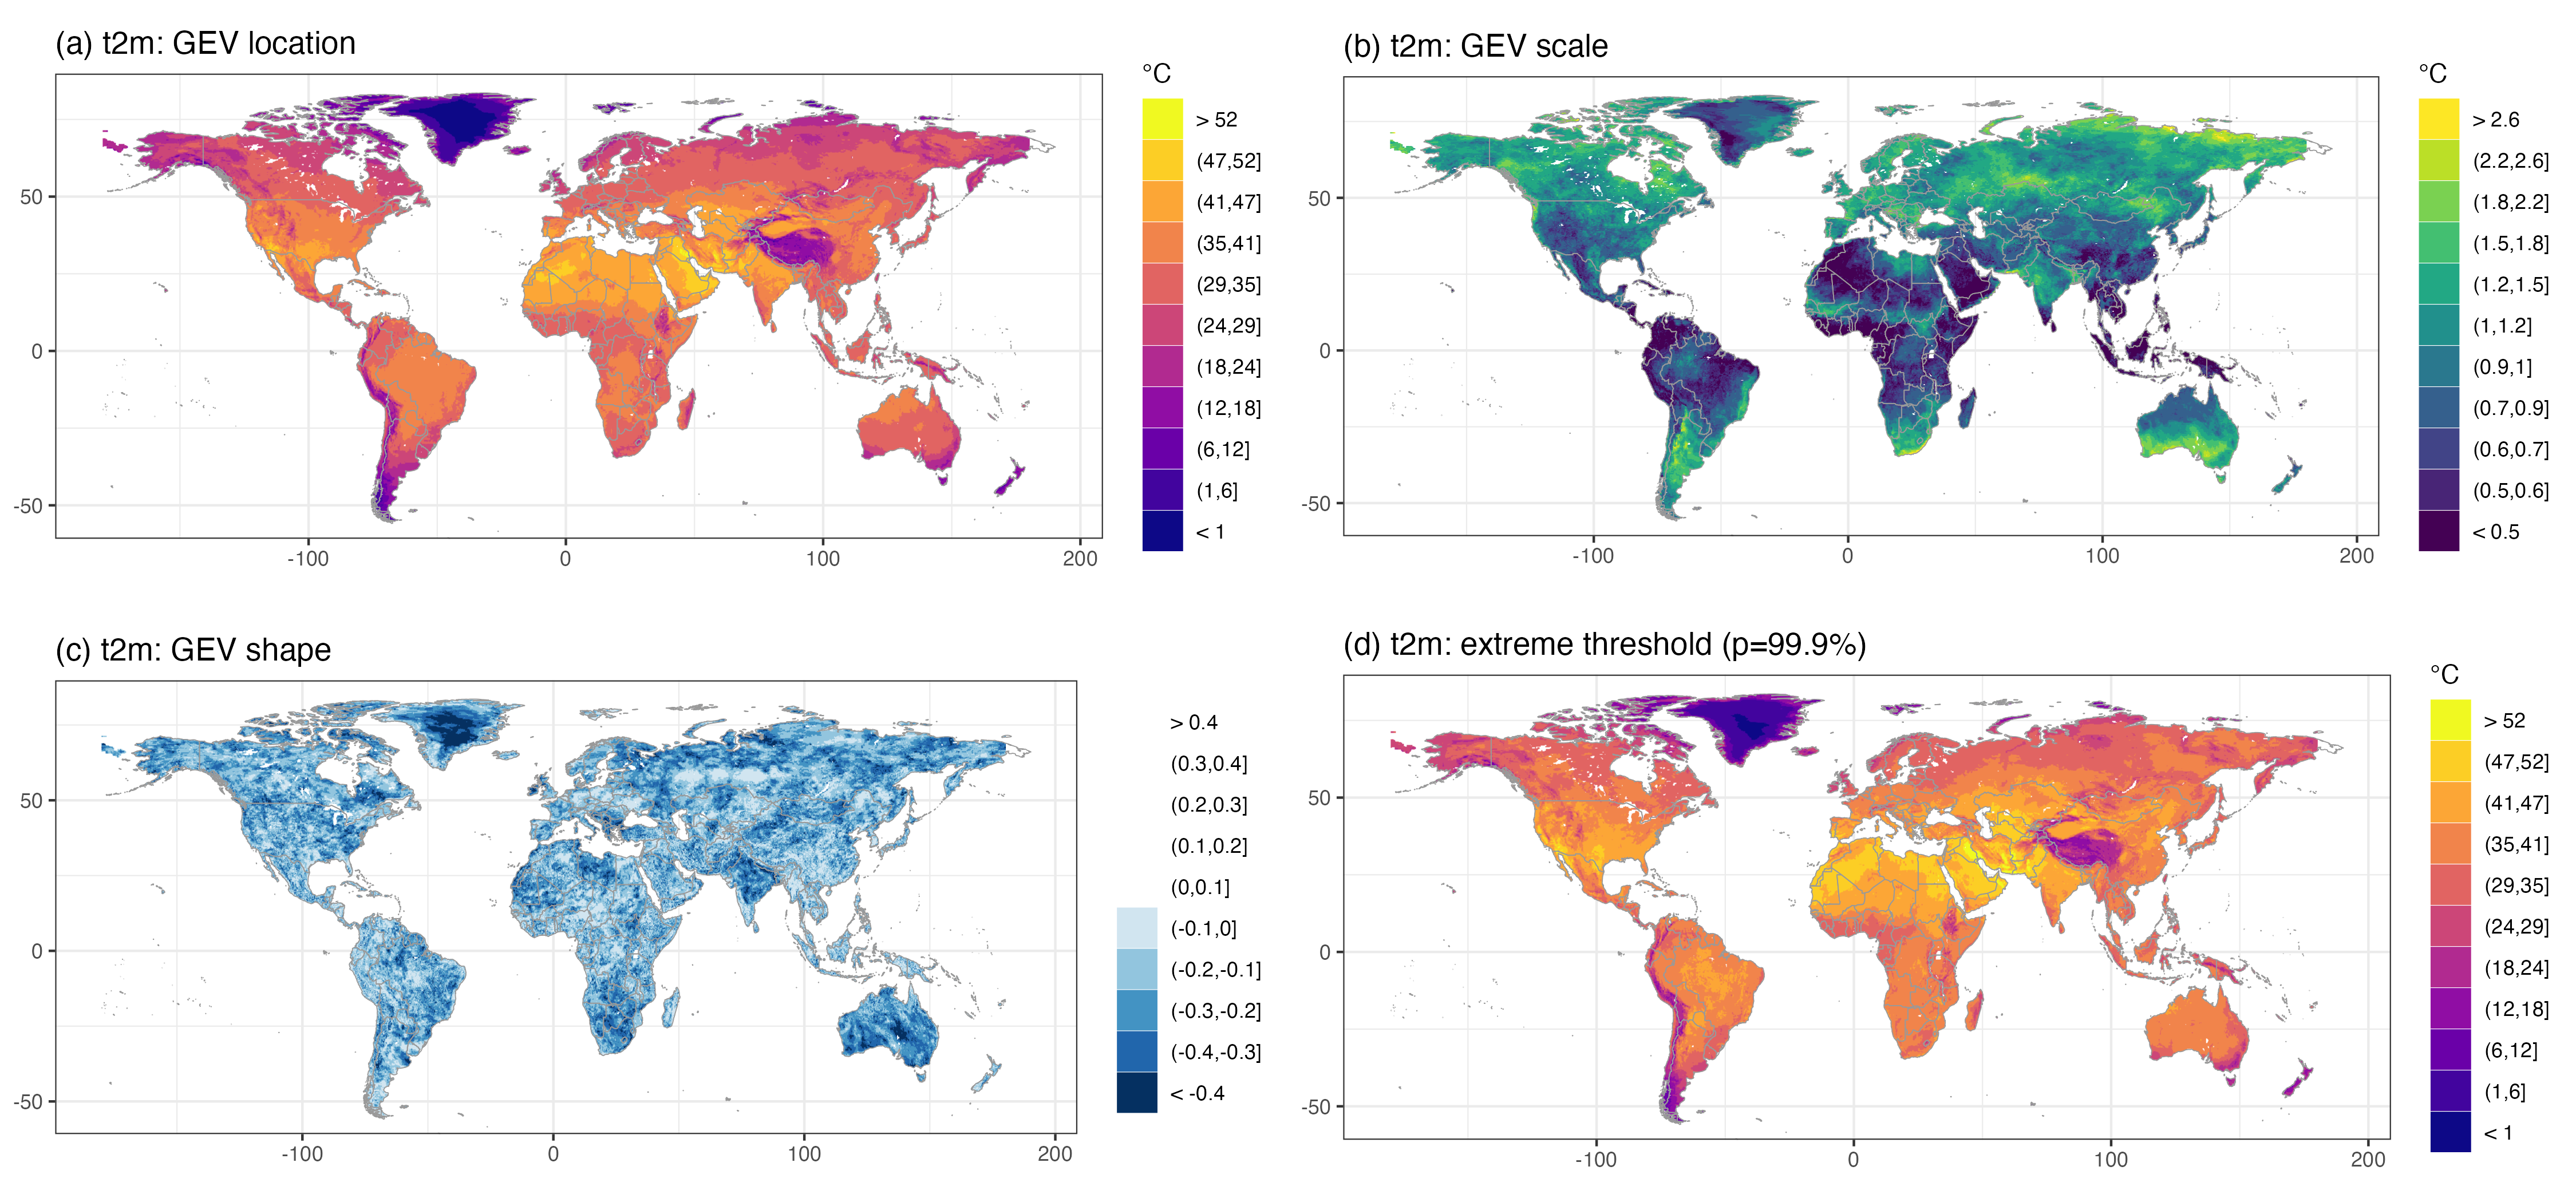
\includegraphics[width=\textwidth]{Figure_GEVfields_t2m_gridbox.png}
%     \caption{Best estimates (posterior medians) of the IFS-GEV fields and extreme thresholds for 2m temperature.}
%     \label{fig:bestGEVt2m}
% \end{figure}
% \begin{figure}[!t]
%     \centering
%     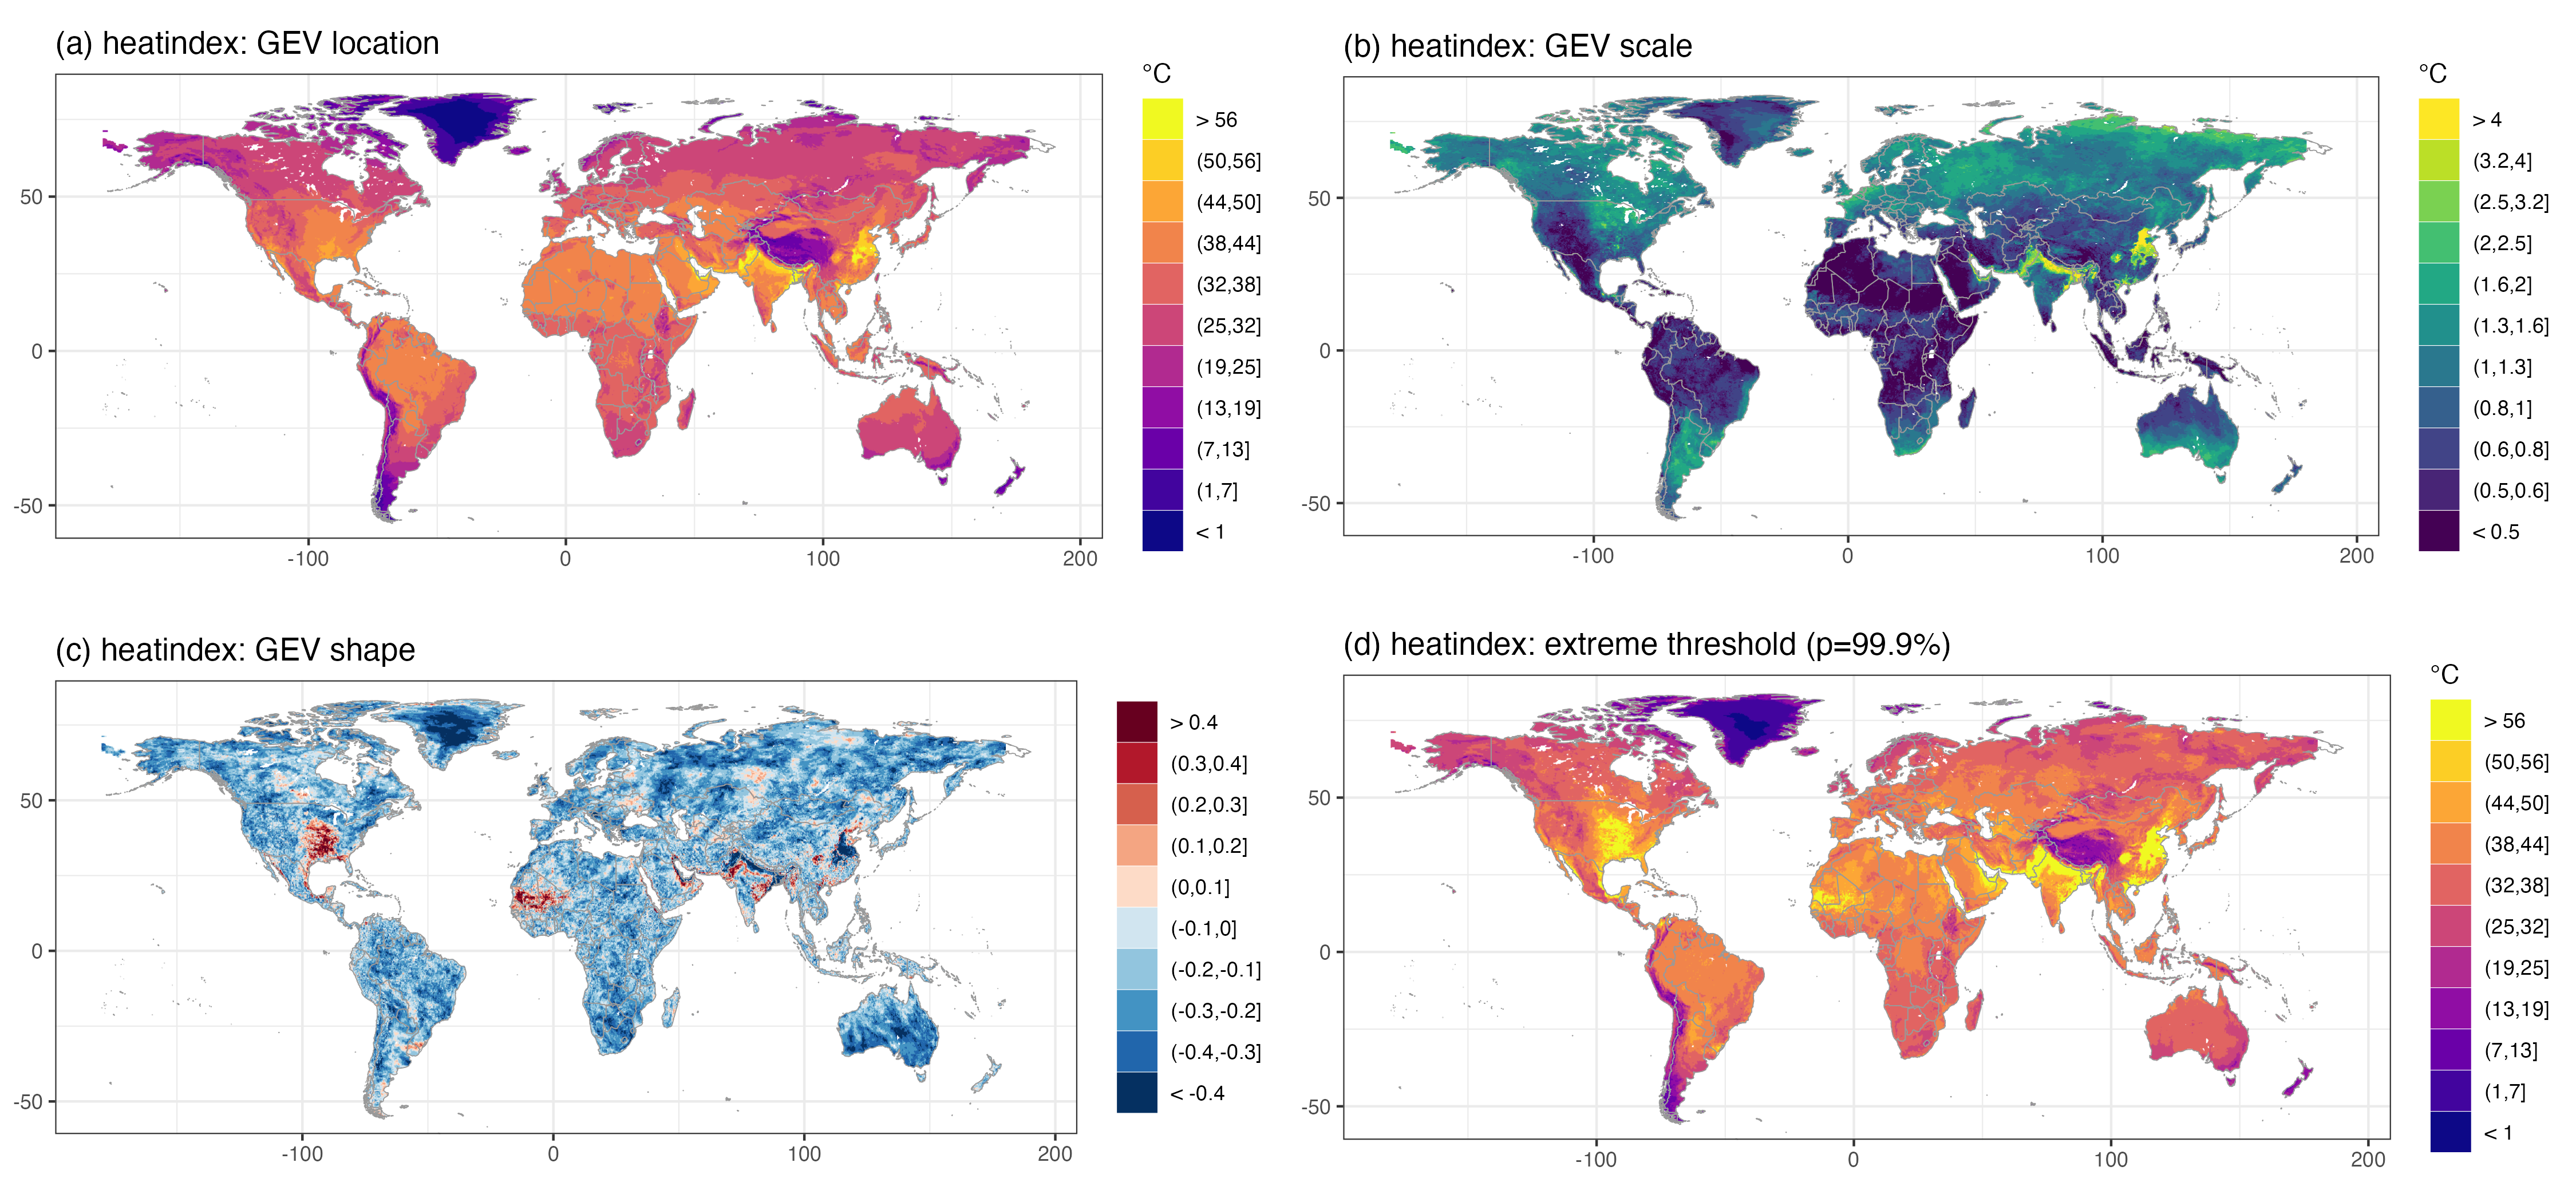
\includegraphics[width=\textwidth]{Figure_GEVfields_heatindex_gridbox.png}
%     \caption{Best estimates (posterior medians) of the IFS-GEV fields and extreme thresholds for the heat index.}
%     \label{fig:bestGEVheatindex}
% \end{figure}

% \section{Assessment of HENS realism in Greenland} \label{appdx:greenland}

% % \todo{AM 3/6/2026- can we move the Greenland paragraph to supplemental information, for the sake of space and word limits.}
% The fact that Greenland stands out so clearly with large anomalies relative to ERA5 in Figure~\ref{fig:threeversions} and \textit{exceptionally unlikely} temperatures relative to IFS-GEV in Figure~\ref{fig:probcontain} motivates us to examine the realism of emulated temperatures in this region more thoroughly. Figure~\ref{supp:fig:promice2} shows how ERA5, IFS, and HENS data compare with extreme gauge-based two-meter surface temperatures from the  Programme for Monitoring of the Greenland Ice Sheet \cite[PROMICE;][]{Fausto2021,How2022data} database. In 2023, paired comparisons of model grid box with nearest-neighbor PROMICE sites show good agreement between all three data sources and the extreme gauged-based 2m temperatures from PROMICE. The HENS extreme temperature distributions overlap the 2023 PROMICE maxima for 24 of the 32 sites; HENS distributions contain the all-time PROMICE maxima for 29 of 38 sites. Figure~\ref{supp:fig:promice1} summarizes the annual cycle of monthly maximum 2m and surface air temperatures, which shows that the difference between surface and 2m temperatures can exceed 20$^\circ$C in the summer: this is well in line with the 2m air temperatures simulated by HENS. Therefore, we can be confident that HENS is generating realistic high-latitude temperatures in places like Greenland.


% % \clearpage

% \section{Supplemental figures}

% \begin{figure*}[!h]
% \centering
% 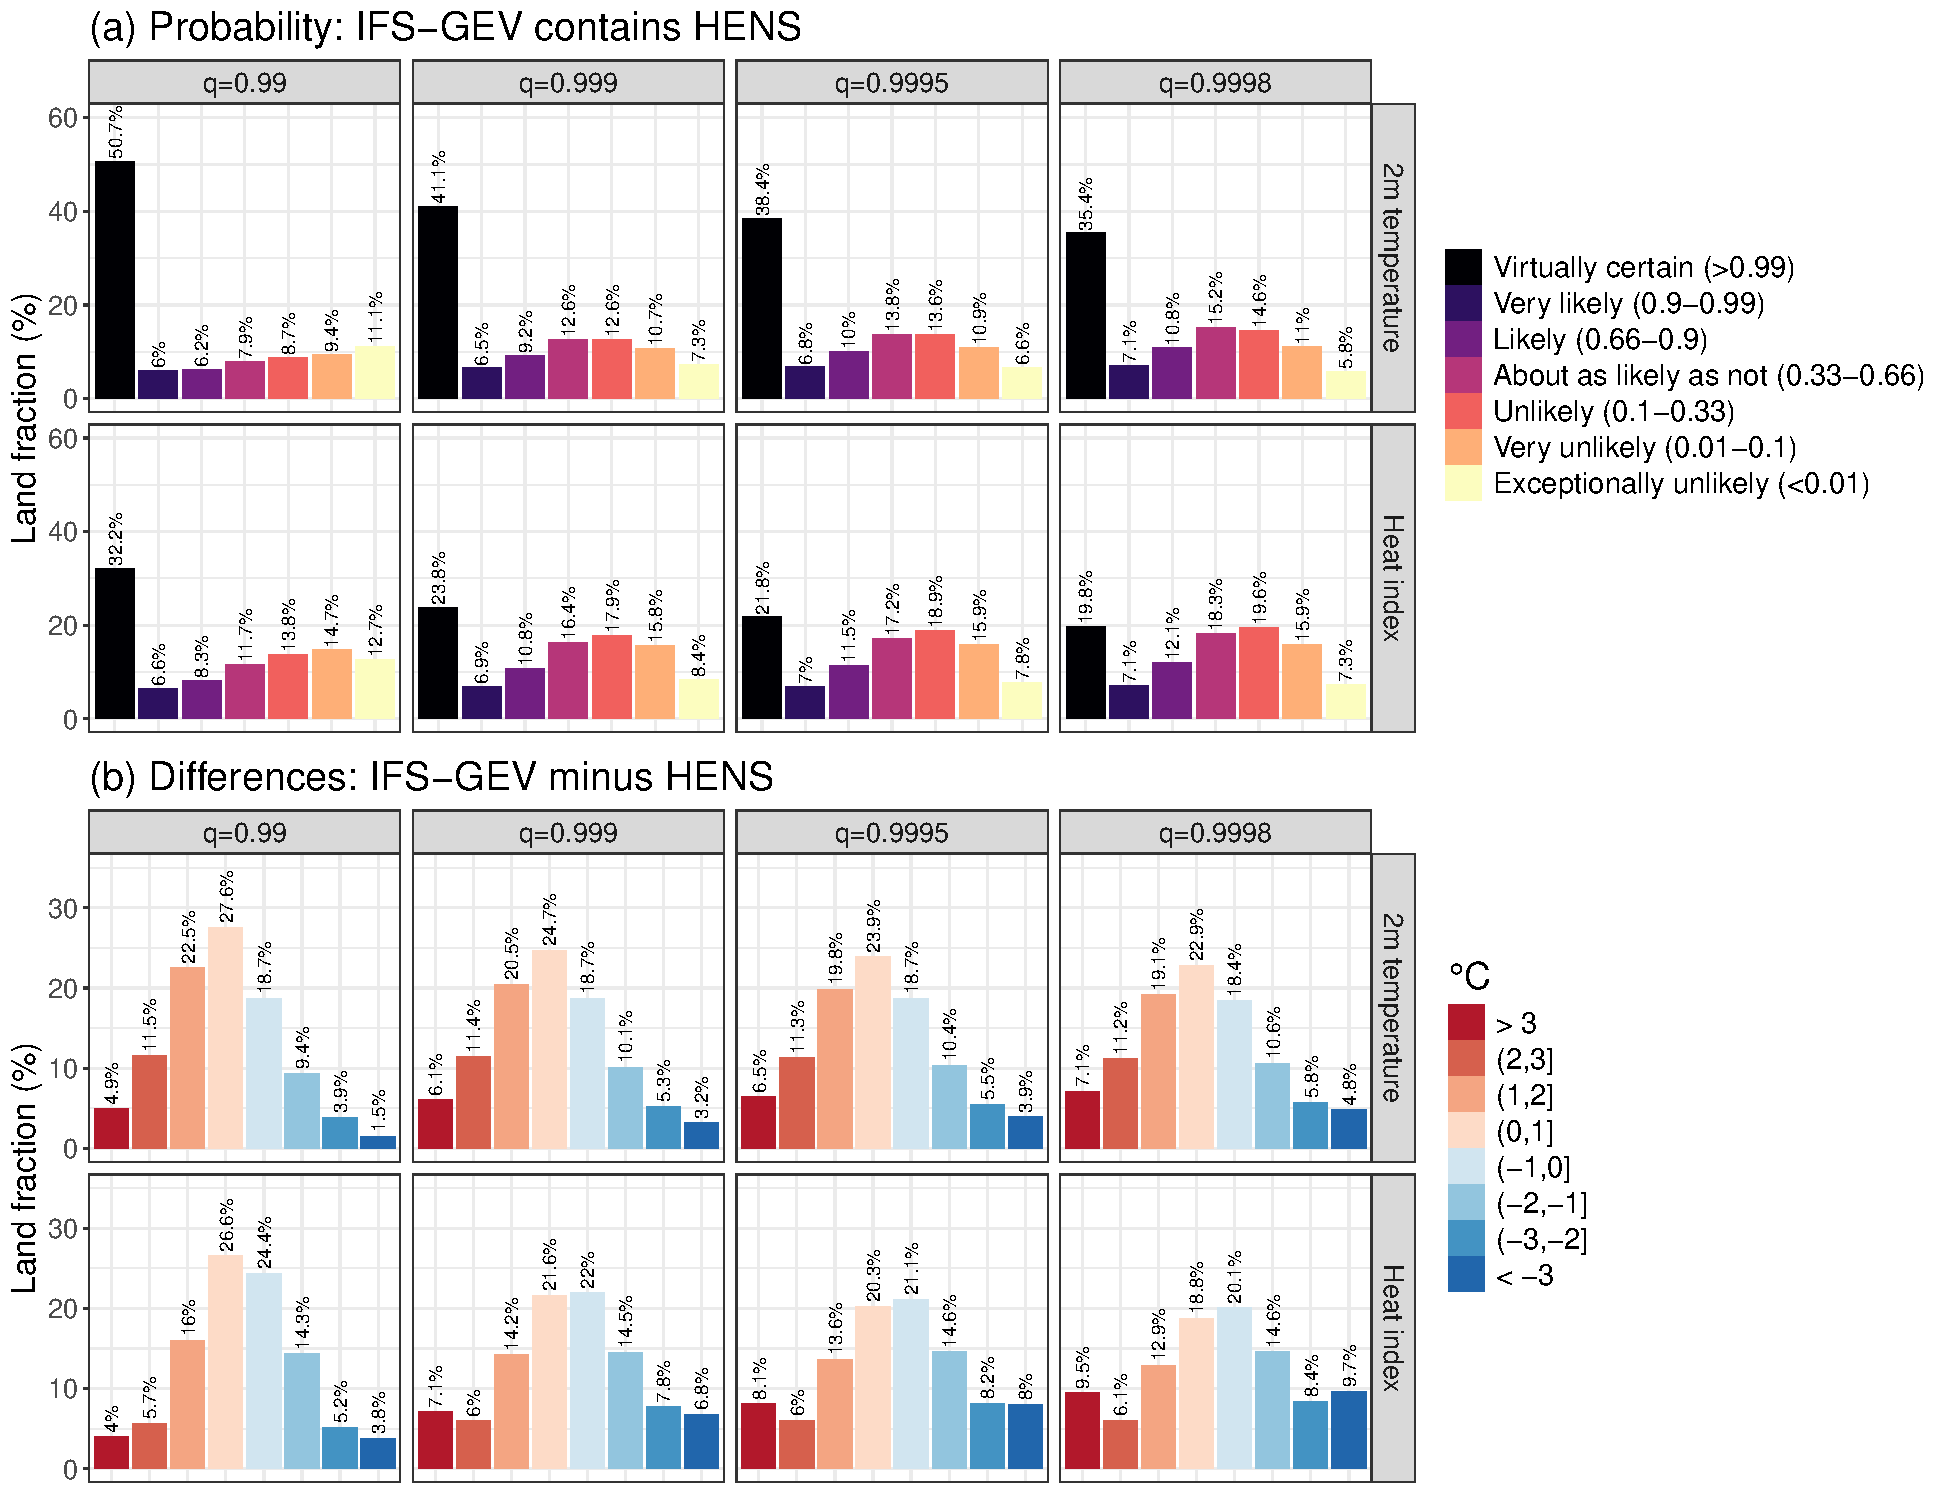
\includegraphics[width = \textwidth]{Figure_IFS_GEV_probContain_HENS_barchart.pdf}
% \caption{Tally of the land fraction falling into each category for probability of containment (panel a.) and differences (panel b.) when comparing IFS-GEV and HENS return levels. In panel (a), lighter colors indicate that HENS estimates are less likely relative to IFS-GEV.}
% \label{fig:barchart}
% \end{figure*}

% \begin{figure}[!h]
%     \centering
%     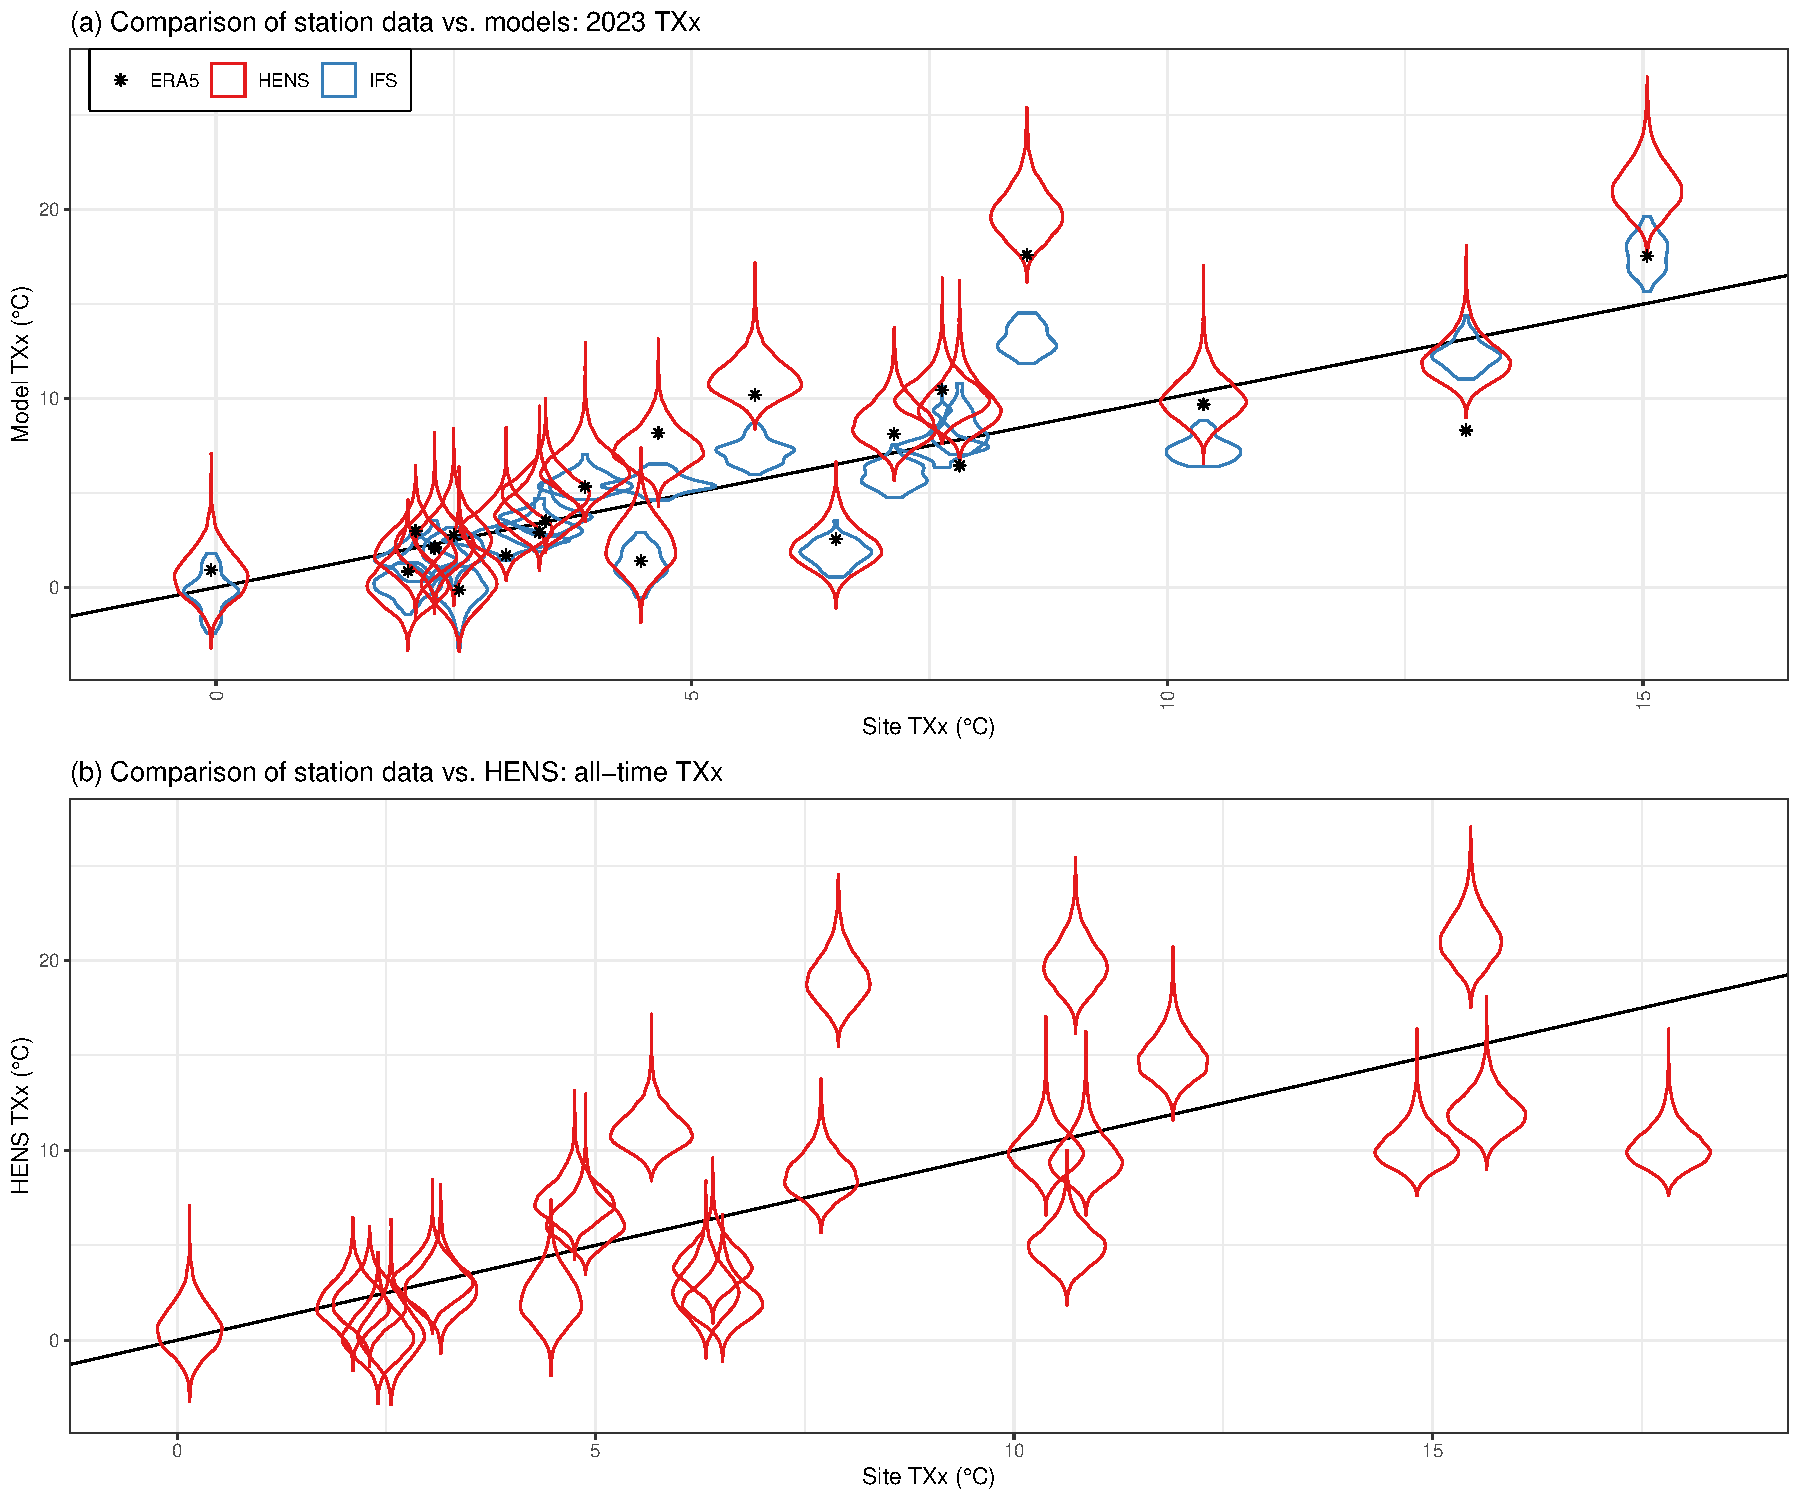
\includegraphics[width=\textwidth]{Figure_PROMICE_vs_Models_v2.pdf}
%     \caption{Comparison of the reanalysis and forecast ensemble temperature extremes versus the gauge-based maxima taken from the PROMICE database \citep{Fausto2021,How2022data}, for both 2023 (top) and all-time (bottom).}
%     \label{supp:fig:promice2}
% \end{figure}

% \begin{figure}[!h]
%     \centering
%     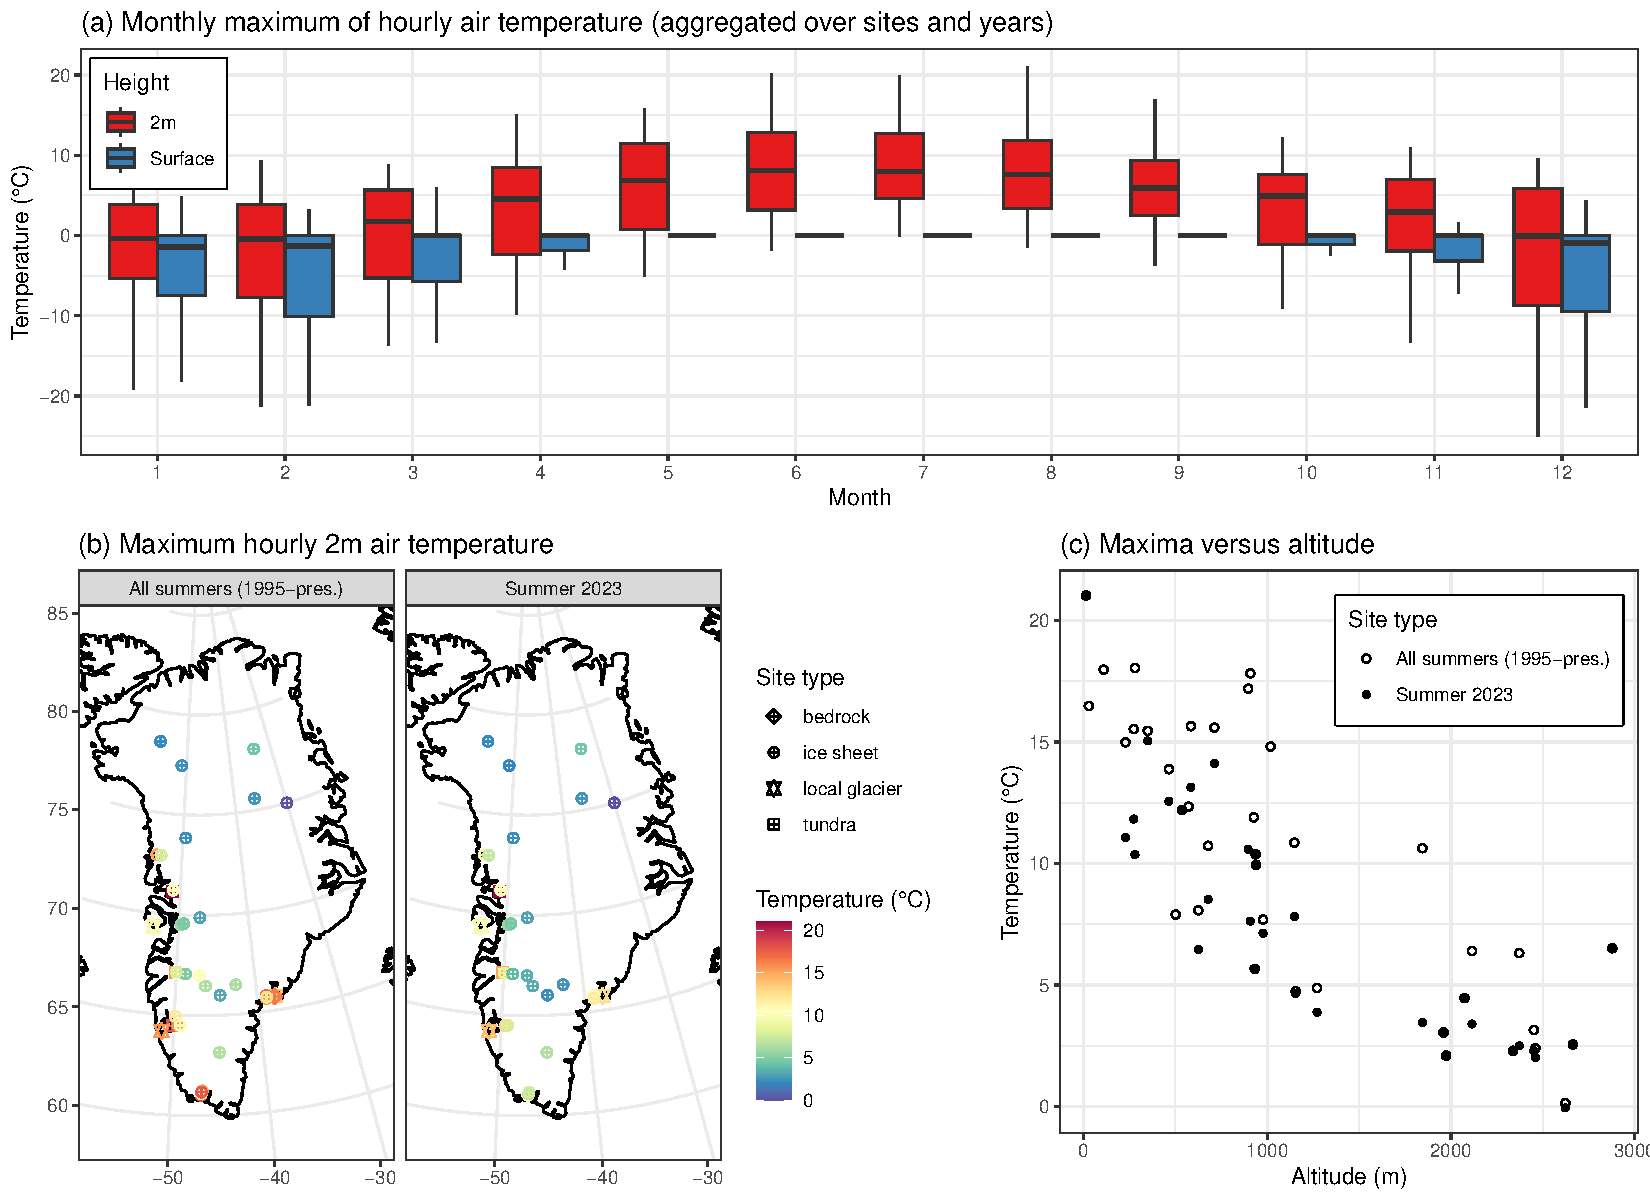
\includegraphics[width=\textwidth]{PROMICE_temperature_extremes_new.pdf}
%     \caption{Summary of monthly maximum two-meter air temperature taken from the PROMICE database \citep{Fausto2021,How2022data} over 1995-2024. Panel (a) shows the annual cycle of two-meter vs. surface temperatures, demonstrating that the difference between two-meter and surface temperatures can get as large as 20$^\circ$ in the summer. Panel (b) shows the spatial distribution of the warmest summertime two-meter air temperatures over Greenland, for both the entire record (1995-present) and the 2023 summer. Panel (c) shows how these temperatures depend on elevation. }
%     \label{supp:fig:promice1}
% \end{figure}



% % \begin{figure*}[!t]
% % \centering
% % 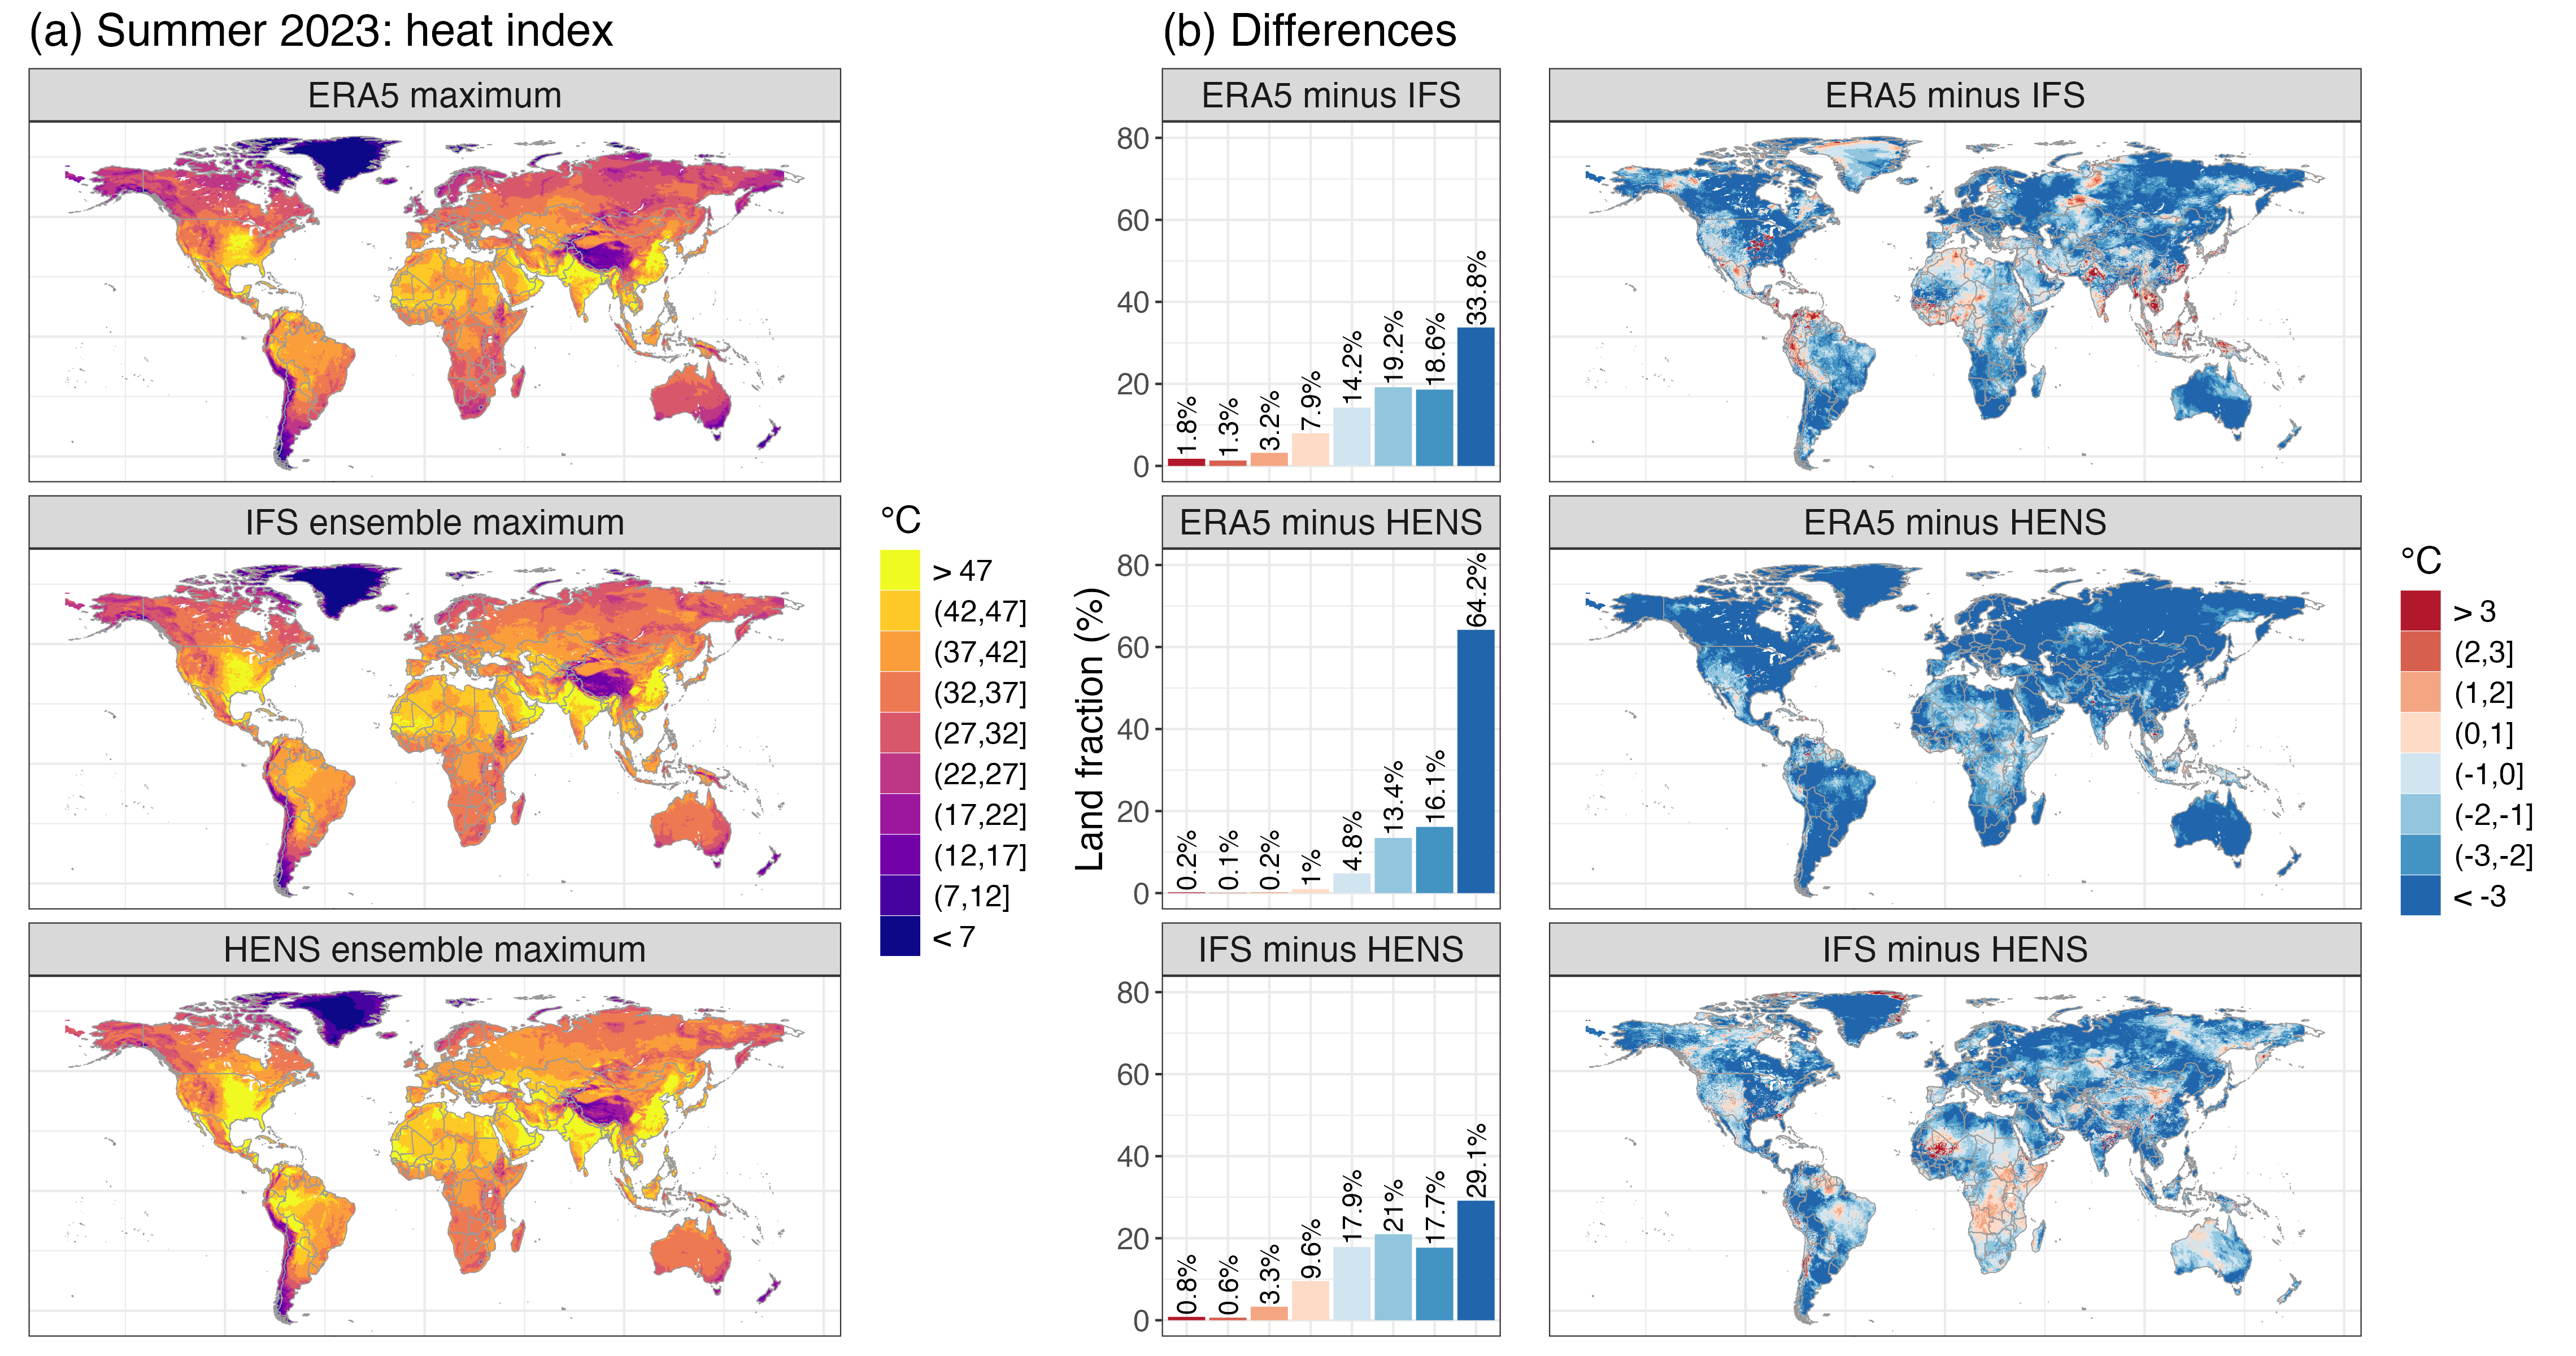
\includegraphics[width = \textwidth]{Figure_heatindex_maxima_diff.png}
% % \caption{Comparison of three different versions of the hottest heat index values temperatures over global land regions from 01 June 2023 to 31 August 2023. Panel (a) shows the hottest heat index from ERA5 (our best reconstructions of the realized temperatures; left), the IFS forecast ensemble (middle), and the HENS ensemble (right). Panel (b) compares the differences between three versions of reality.}
% % \label{fig:threeversions_hi}
% % \end{figure*}


% % \begin{figure}
% %     \centering
% %     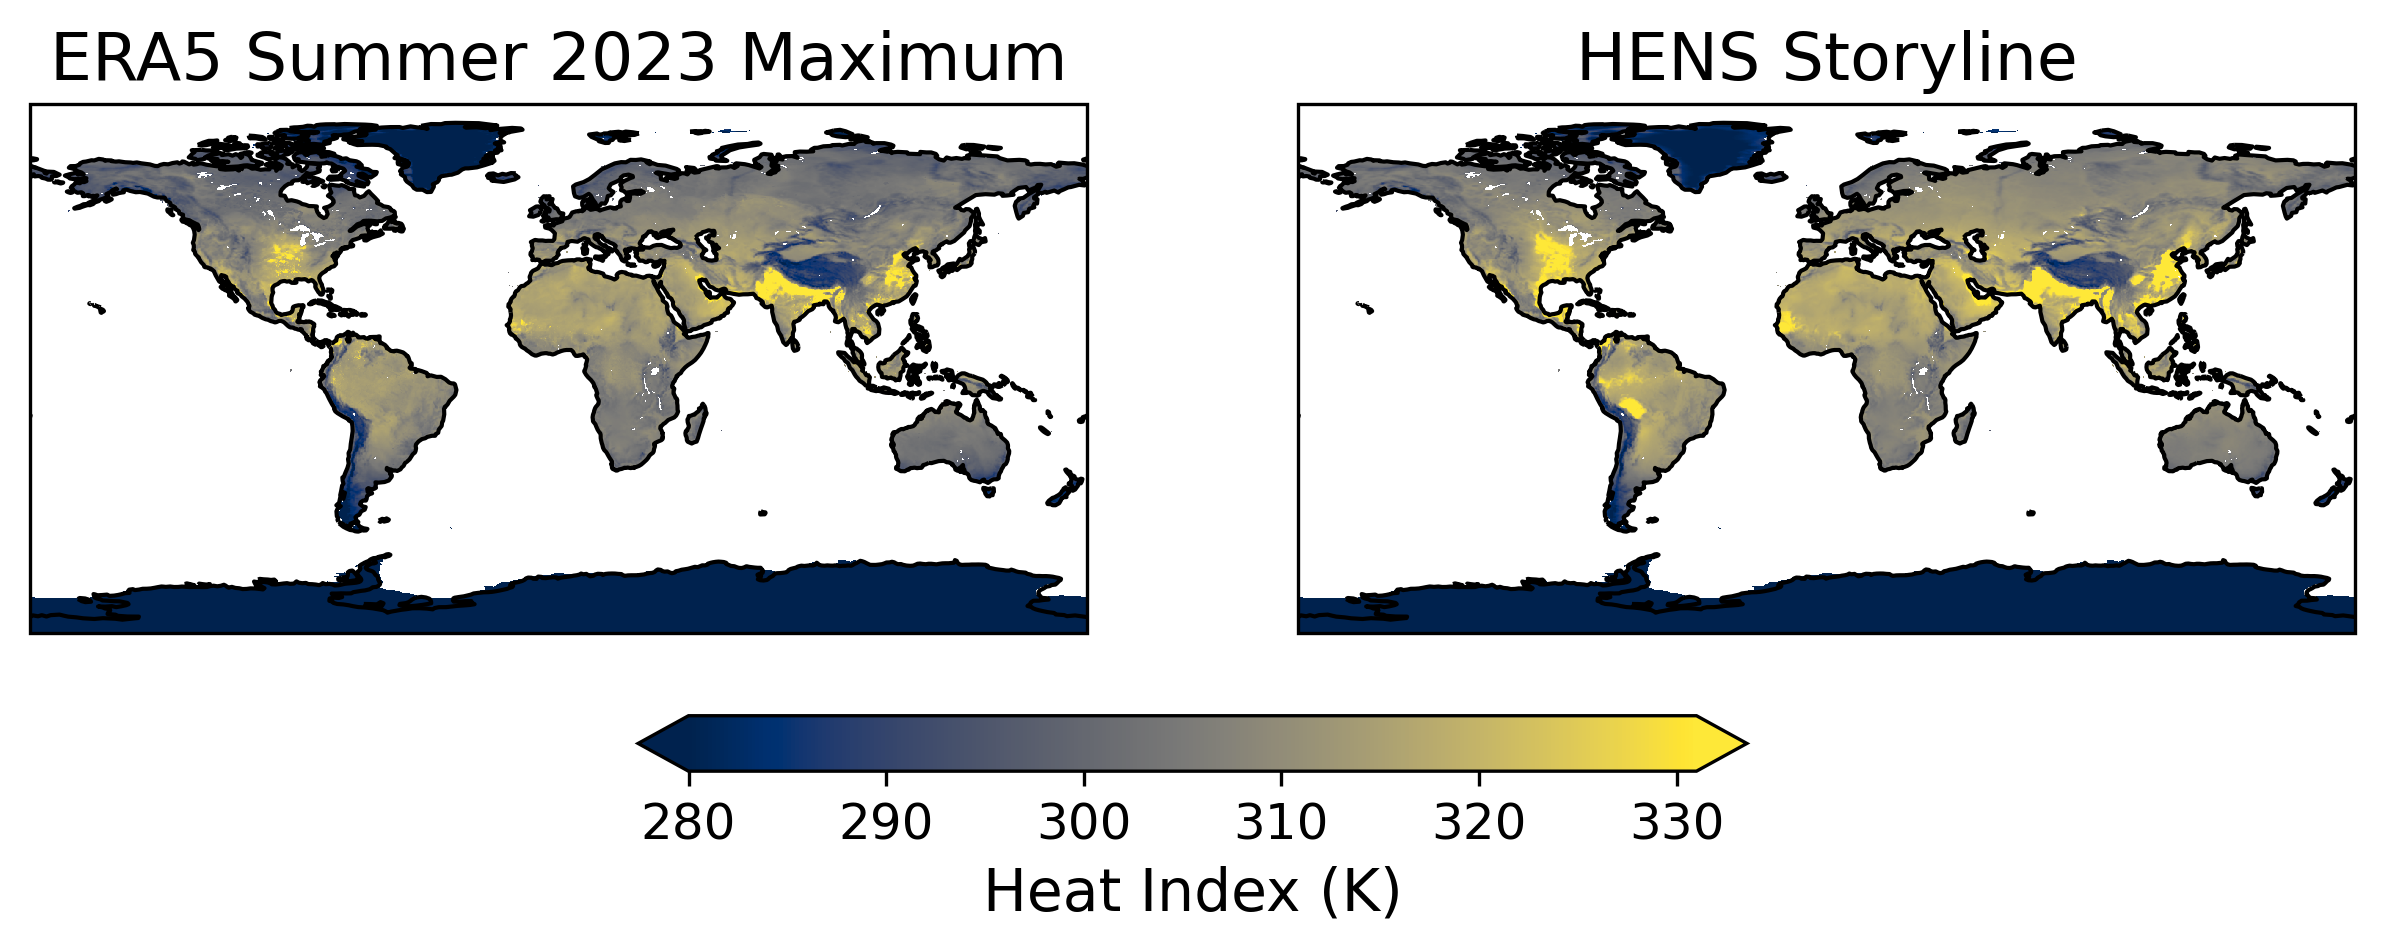
\includegraphics[width=\linewidth]{figures/era5_vs_hens_heatindex.png}
% %     \caption{ERA5 vs. HENS Storyline.}
% %     \label{fig:era5_vs_hens_storyline_raw}
% % \end{figure}

% \begin{figure*}[!t]
% \centering
% 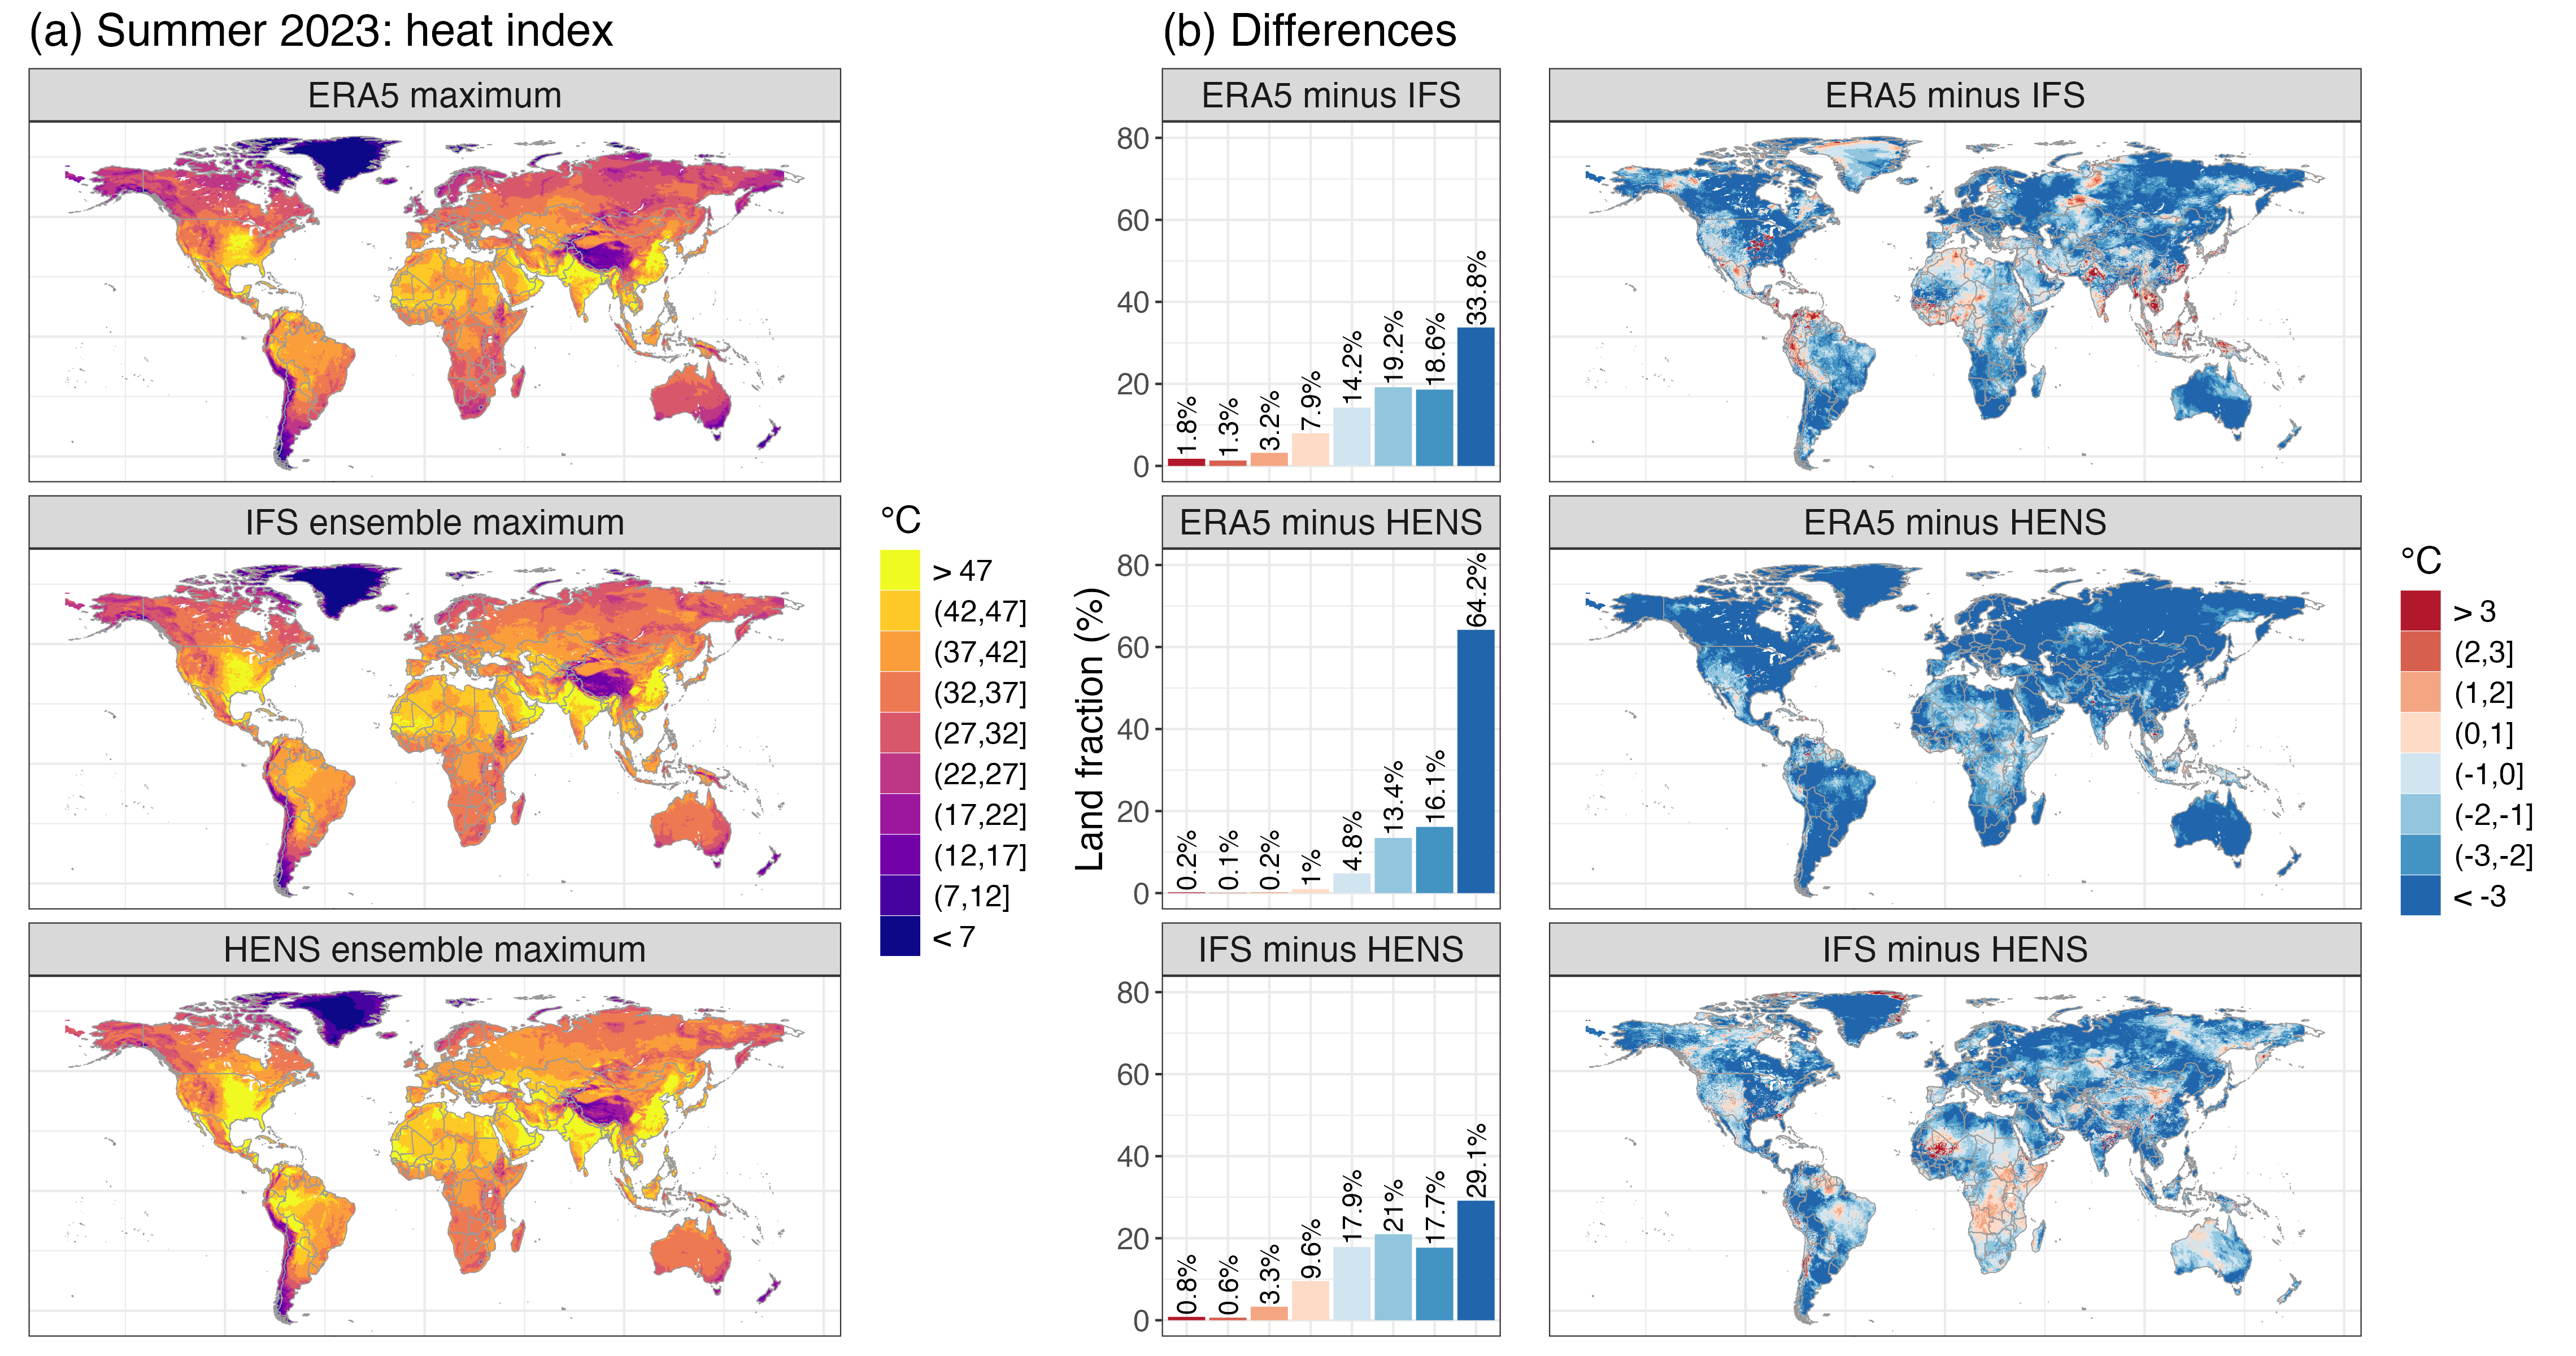
\includegraphics[width = \textwidth]{Figure_heatindex_maxima_diff.png}
% \caption{Same as Figure~\ref{fig:threeversions} but for the heat index.}
% \label{fig:threeversions_heatindex}
% \end{figure*}

% \begin{figure*}[!t]
% \centering
% 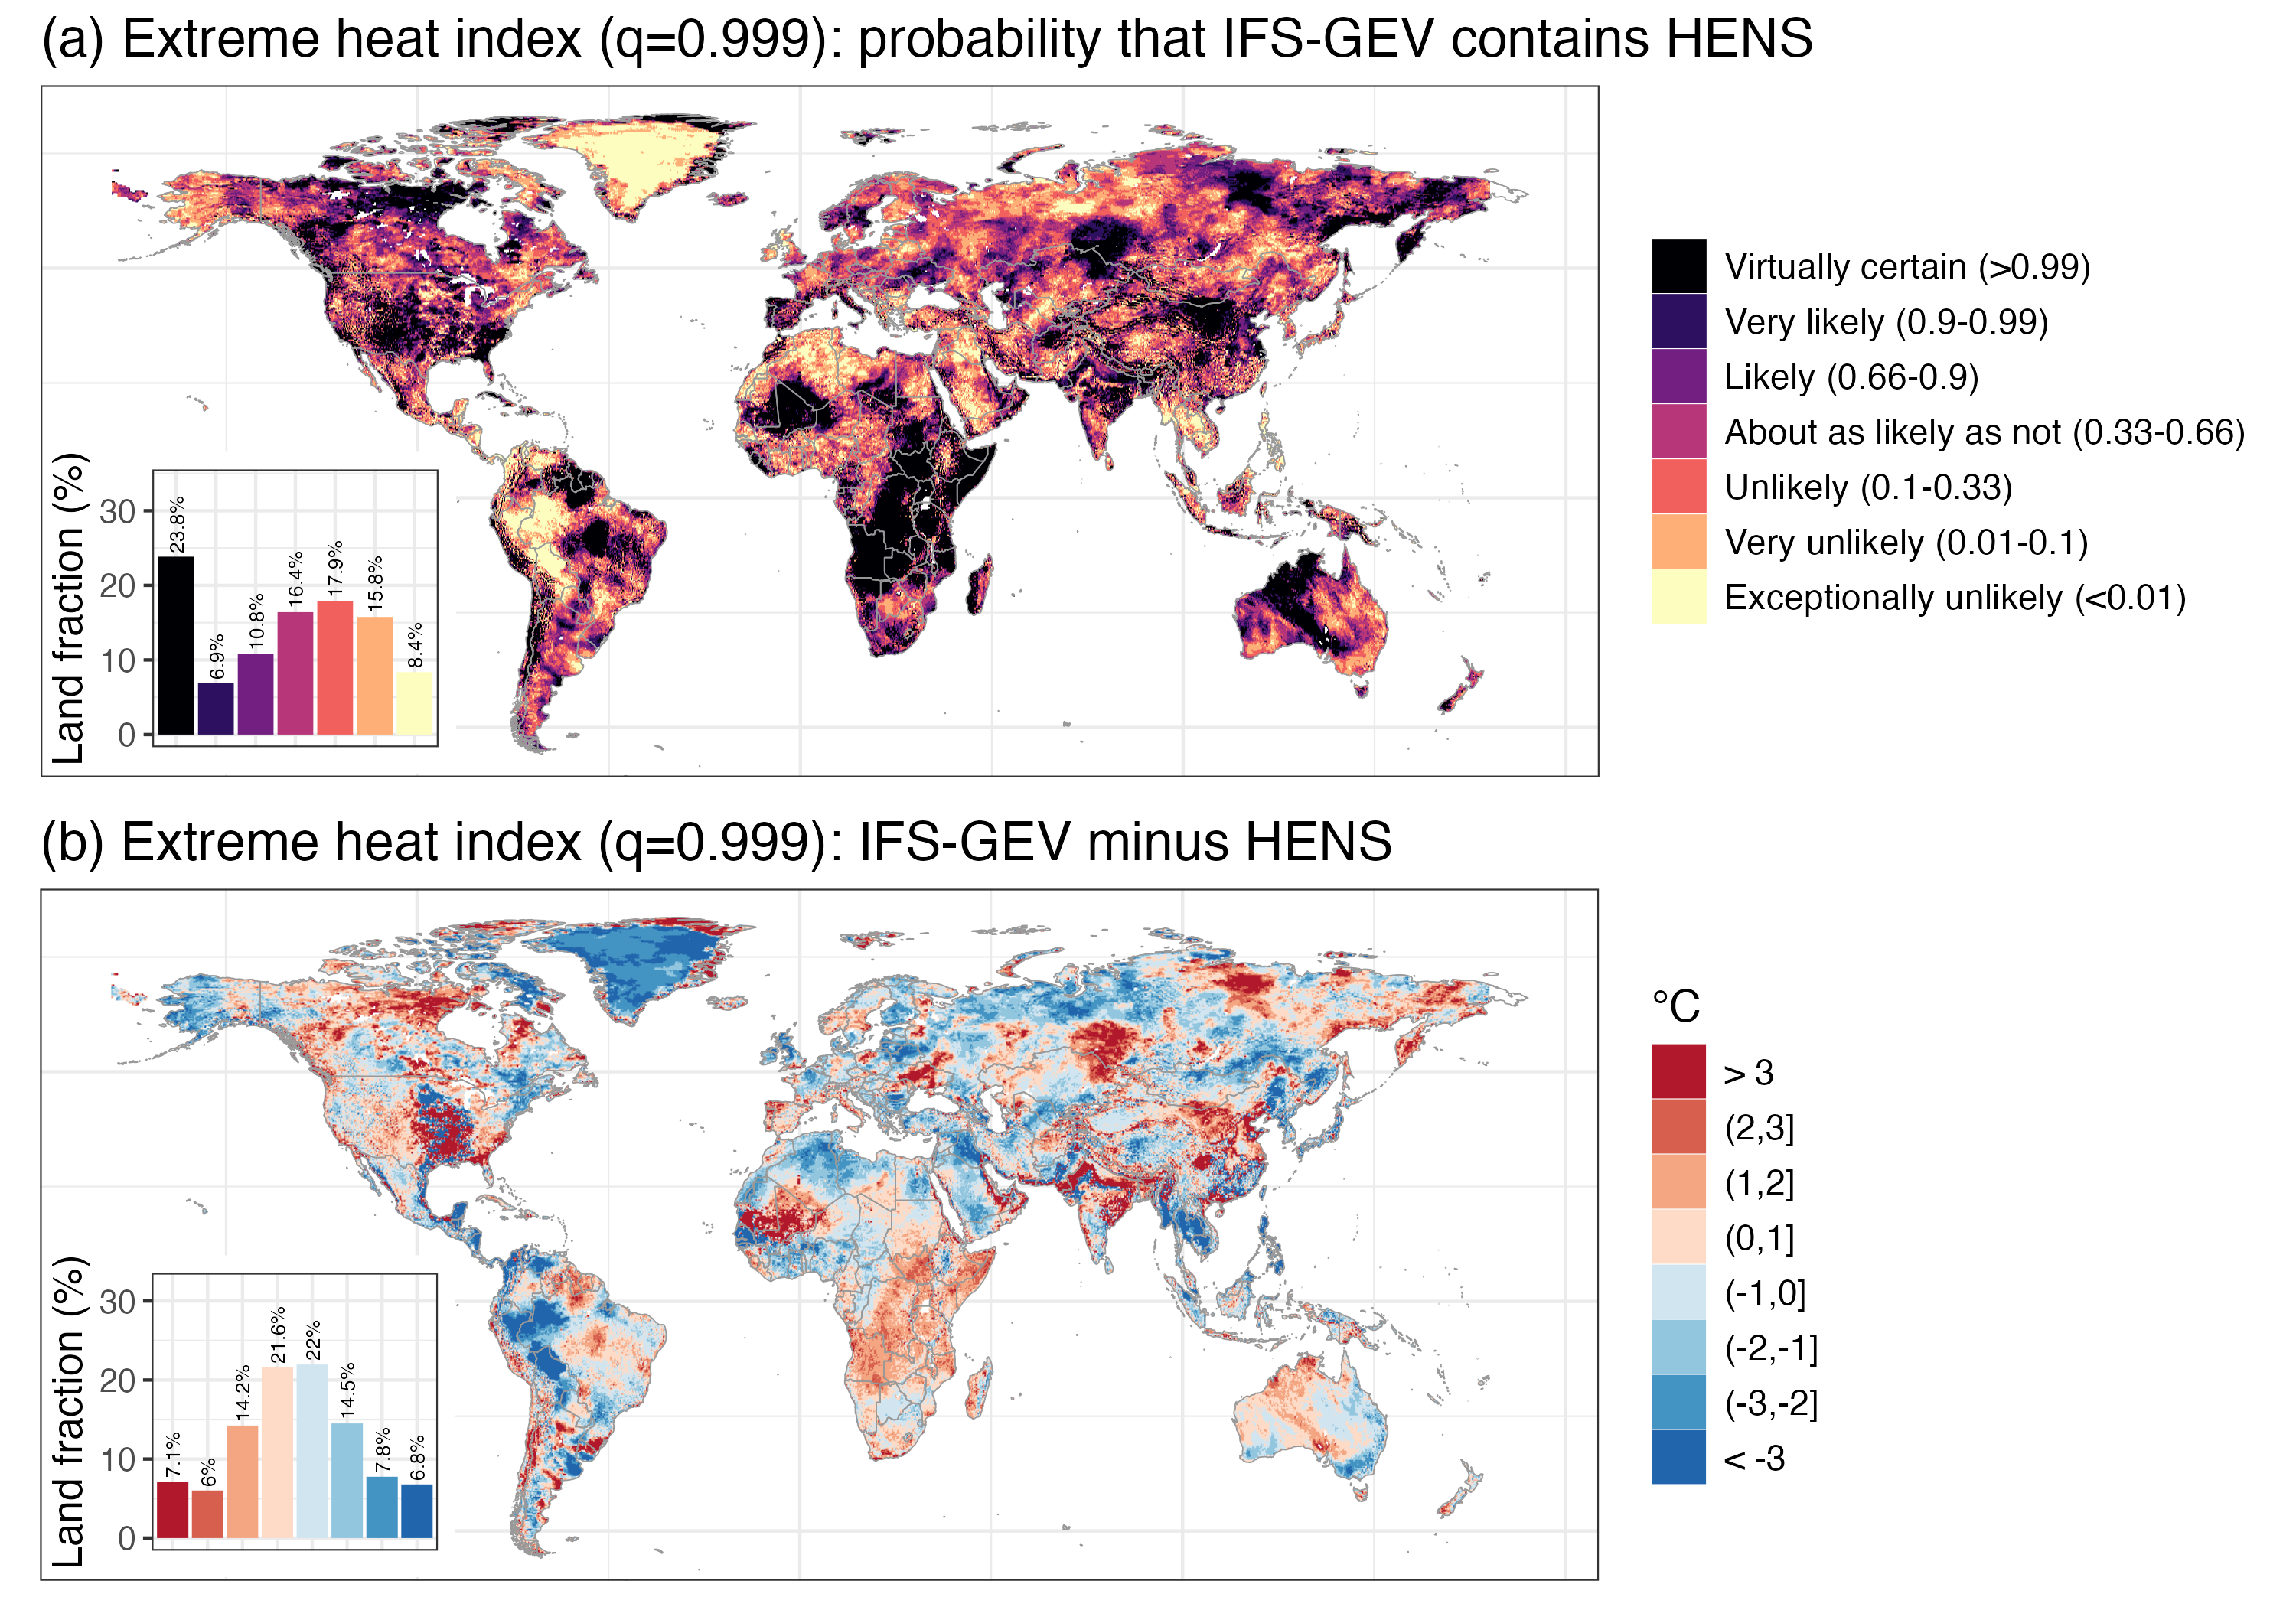
\includegraphics[width = \textwidth]{Figure_heatindex_probContain_1000day.png}
% \caption{Comparison of IFS-GEV extreme event thresholds ($99.9\%$ percentile) for the heat index with corresponding empirical estimates calculated from the HENS ensemble. Panel (a) tallies the probability that the IFS-GEV threshold contains (is larger than) the HENS threshold; lighter colors indicate that HENS values are more extreme than IFS-GEV. Panel (b) tallies the difference in the IFS-GEV event threshold (the posterior median) and the HENS estimate. Panel insets show the land fraction in each color category.}
% \label{fig:probcontain_hi}
% \end{figure*}

% % \begin{figure}
% %     \centering
% %     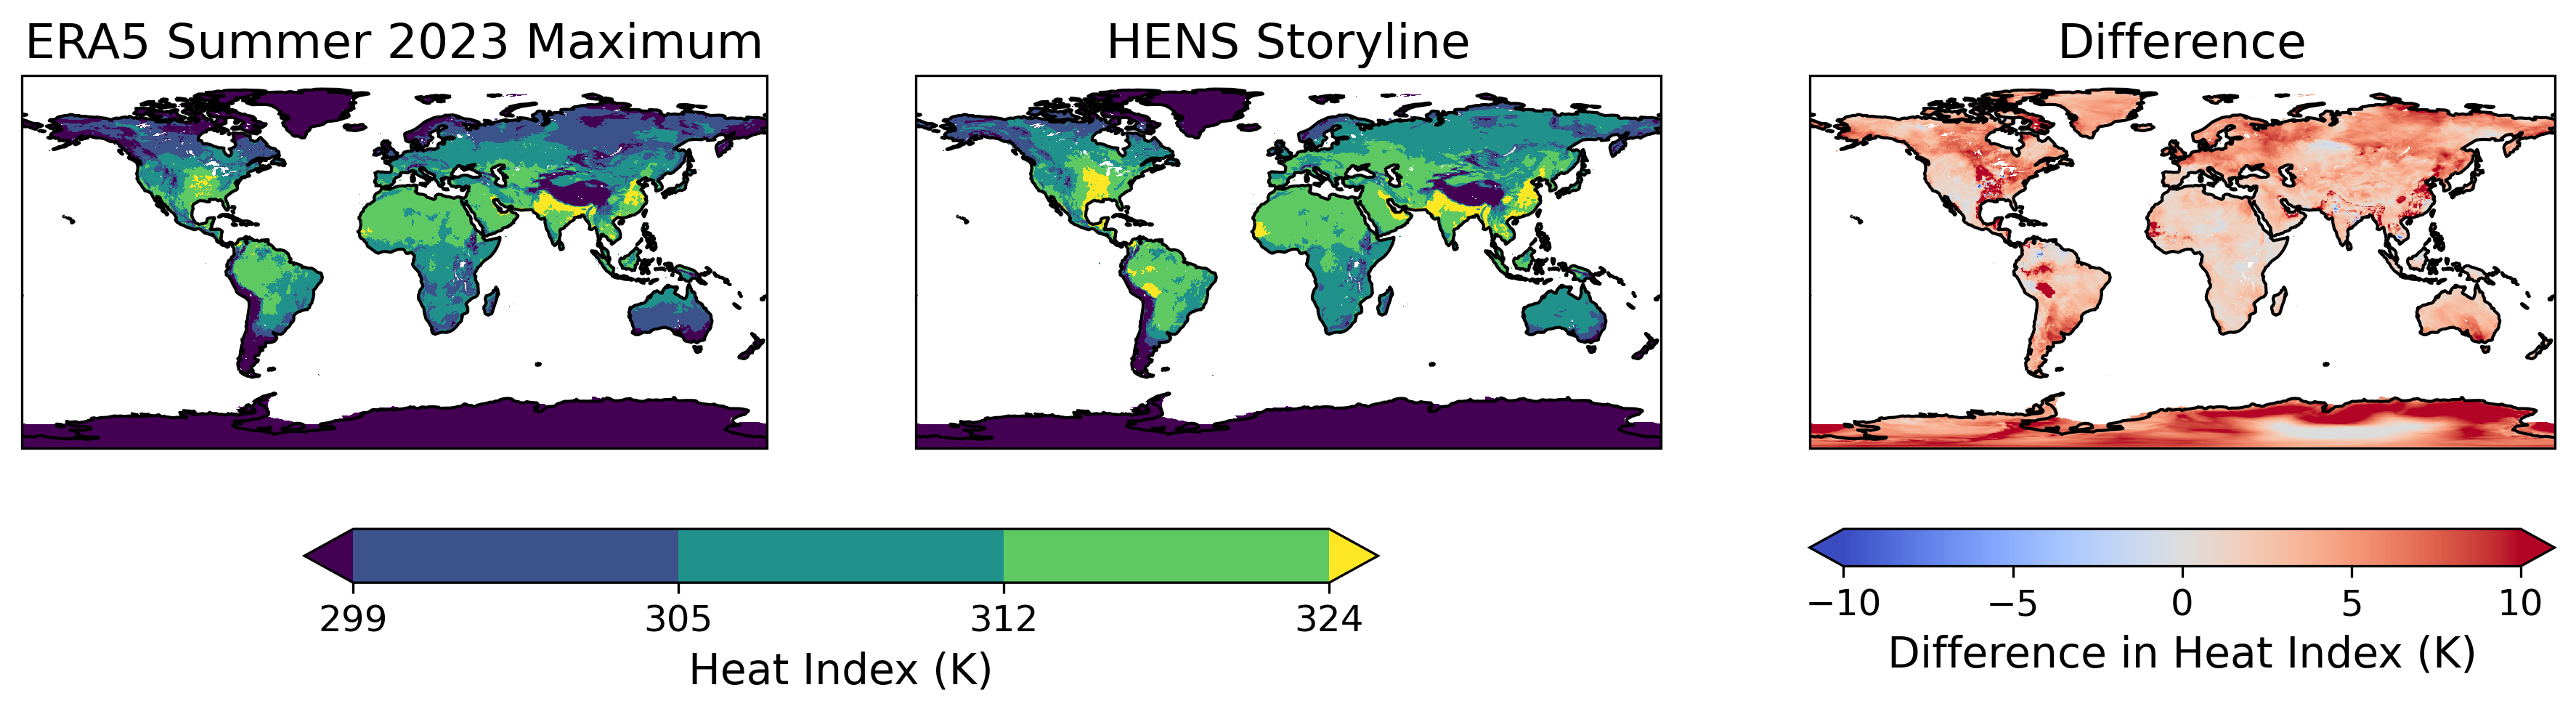
\includegraphics[width=\linewidth]{figures/era5_vs_hens_heatindex_with_diff.png}
% %     \caption{ERA5 vs. HENS Storyline}
% %     \label{fig:era5_vs_hens_heatindex_binned_nws}
% % \end{figure}

% % \begin{figure}
% %     \centering
% %     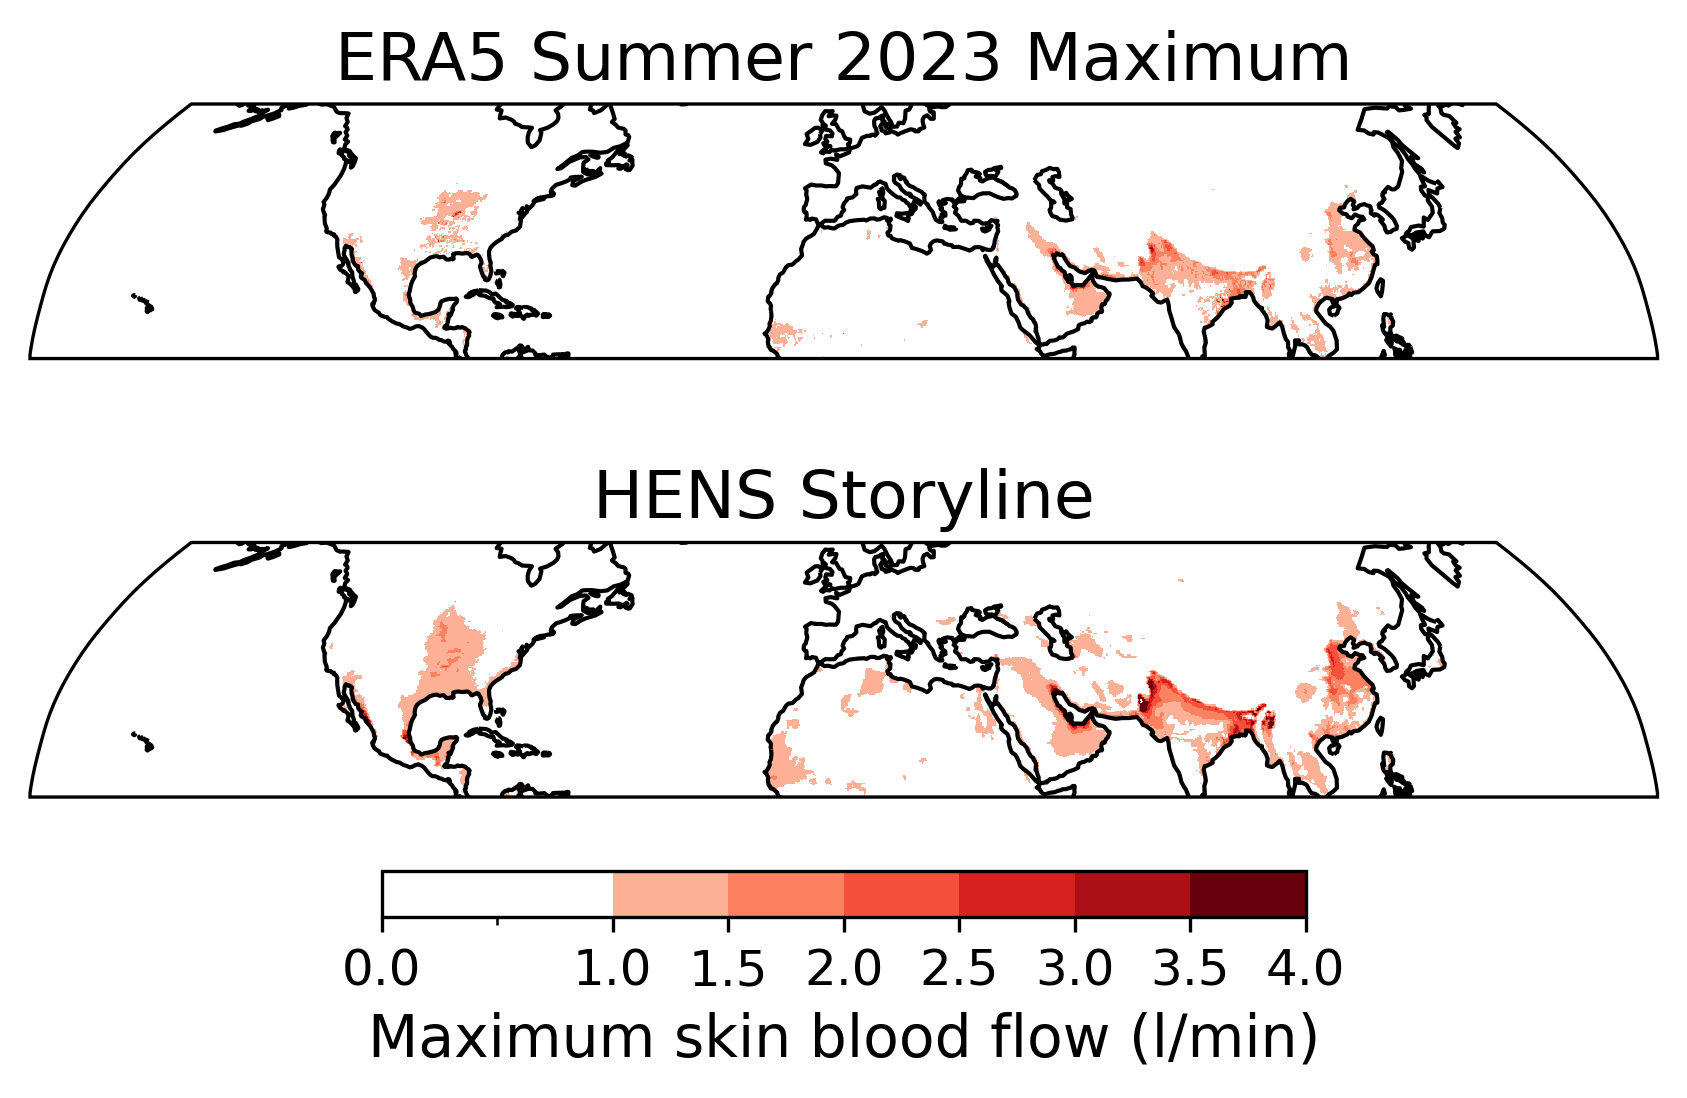
\includegraphics[width=\linewidth]{figures/blood_flow_figure.png}
% %     \caption{ERA5 vs. HENS Storyline of maximum skin blood flow.}
% %     \label{fig:era5_vs_hens_blood_flow}
% % \end{figure}


% % \begin{figure}[!h]
% %     \centering
% %     \includegraphics[width=\textwidth]{Figure_IFS_GEV_probContain_HENS.jpg}
% %     \caption{As in Figure~\ref{fig:probcontain}(a) but for $r$-day return levels with $r\in\{100,1000,2000,\infty\}$.}
% %     \label{supp:fig:probcontain}
% % \end{figure}

% % \begin{figure}[!h]
% %     \centering
% %     \includegraphics[width=\textwidth]{Figure_IFS_GEV_diff_HENS.jpg}
% %     \caption{As in Figure~\ref{fig:probcontain}(b) but for $r$-day return levels with $r\in\{100,1000,2000,\infty\}$.}
% %     \label{supp:fig:diff}
% % \end{figure}

% \clearpage

% \section{Supplemental tables}

% \begin{table}[!h]
% \caption{Variables saved in the HENS Output.}
% \centering
% \begin{tabular}{l l l c}
% \hline
% \textbf{Variable}          & \textbf{Units}            & \textbf{Description}                    \\ \hline
% \texttt{t2m}               & K                        & 2m temperature                          \\
% \texttt{d2m}               & K                        & 2m dew point temperature                \\ 
% \texttt{tcwv}              & kg/m²                    & Total column water vapor                \\
% \texttt{t850}              & K                        & Temperature at 850 hPa                  \\
% \texttt{z500}              & m²/s²                    & Geopotential at 500 hPa                 \\
% \texttt{z300}              & m²/s²                    & Geopotential at 300 hPa                 \\
% \texttt{msl}               & Pa                       & Mean sea level pressure                 \\
% \texttt{t500}              & K                        & Temperature at 500 hPa                  \\
% \texttt{sp}                & Pa                       & Surface pressure                        \\
% \texttt{ivt}               & kg/(m·s)                 & Integrated vapor transport              \\
% \texttt{heat\_index}       & K                        & Heat index                              \\
% \texttt{wind\_speed10m}       & m/s                      & 10m wind speed                          \\ \hline
% \end{tabular}
% \label{table:variables}
% \end{table}


% \begin{table}[]
%     \centering
%     \begin{tabular}{c c}
%  \hline
% \textbf{HENS quantile} & \textbf{Fraction of ERA5 t2m maximum contained by HENS} \\ \hline
%       $1 - 1/10 = 0.9$   &         $0.790$ \\
%      $1 - 1/20 = 0.95$   &         $0.854$ \\
%      $1 - 1/50 = 0.98$   &         $0.906$ \\
%     $1 - 1/100 = 0.99$   &         $0.932$ \\
%   $1 - 1/1000 = 0.999$   &         $0.978$ \\
%  $1 - 1/2000 = 0.9995$   &         $0.984$ \\ 
%  $1 - 1/5000 = 0.9998$   &         $0.989$ \\
% Ensemble maximum & $0.994$ \\ \hline
%     \end{tabular}
%     \caption{The land fraction of the globe for which the 2m temperature HENS quantile contains the ERA5 summertime maximum t2m. We note that the containment fraction levels out for quantiles beyond $0.999$ (percentiles beyond $99.9\%$).}
%     \label{tab:henscontain}
% \end{table}

%  %    Quantile FracContain_era5
%  %      1 - 1/10 = 0.9            0.790
%  %     1 - 1/20 = 0.95            0.854
%  %     1 - 1/50 = 0.98            0.906
%  %    1 - 1/100 = 0.99            0.932
%  %  1 - 1/1000 = 0.999            0.978
%  % 1 - 1/2000 = 0.9995            0.984
%  % 1 - 1/5000 = 0.9998            0.989
%  %       Ensemble max.            0.994

% \end{appendix}

\end{document}



